\documentclass[a4paper,11pt]{report}
% Compiled with tectonic (XeTeX): use fontspec with Latin Modern, loaded by OTF filename
% (font-by-name lookup fails here, no fontconfig). fontenc+inputenc+lmodern under XeTeX
% mis-renders « » § ² (they showed as ń ż ğ š); fontspec renders all Unicode natively.
\usepackage{fontspec}
\setmainfont{Latin Modern Roman}[Extension=.otf, UprightFont=lmroman10-regular, BoldFont=lmroman10-bold, ItalicFont=lmroman10-italic, BoldItalicFont=lmroman10-bolditalic]
\setsansfont{Latin Modern Sans}[Extension=.otf, UprightFont=lmsans10-regular, BoldFont=lmsans10-bold, ItalicFont=lmsans10-oblique]
\setmonofont{Latin Modern Mono}[Extension=.otf, UprightFont=lmmono10-regular, BoldFont=lmmonolt10-bold, ItalicFont=lmmono10-italic]
\usepackage[french]{babel}
\usepackage{graphicx}
\usepackage{float}
\usepackage{amsmath}
\usepackage{booktabs}
\usepackage{tabularx}
\usepackage{array}
% Numérotation plate des figures/tableaux (Figure 1..N, pas 2.1) : la classe report réinitialise
% et préfixe les compteurs par chapitre ; chngcntr les détache pour une numérotation continue,
% cohérente avec les renvois « Figure N » du texte et le rendu docx.
\usepackage{chngcntr}
\counterwithout{figure}{chapter}
\counterwithout{table}{chapter}
\usepackage[most]{tcolorbox}
\usepackage{soul}
% Titre de chapitre sur la même ligne que « Chapitre N » (au lieu du numéro seul au-dessus du titre)
\usepackage{titlesec}
\titleformat{\chapter}[hang]{\normalfont\LARGE\bfseries}{\chaptertitlename\ \thechapter.}{0.6em}{}
\titlespacing*{\chapter}{0pt}{0pt}{1.5em}
% Légendes : séparateur deux-points à la française (« Figure 1 : ... », format demandé),
% et non « Figure 1 – » (le tiret de babel-french) ni « Figure 1. »
\usepackage{caption}
\DeclareCaptionLabelSeparator{frcolon}{~: }
\captionsetup{labelsep=frcolon, font=small, labelfont=bf}
\usepackage{geometry}
\geometry{margin=2.5cm}
% Grands tableaux (>= 7 colonnes) tournés en page paysage pour rester lisibles
\usepackage{pdflscape}
\usepackage{hyperref}
\hypersetup{hidelinks}
% URL / DOI cassables n'importe ou (bibliographie), dans la police du corps
\usepackage{xurl}
\urlstyle{same}
\sethlcolor{yellow}
\setlength{\parindent}{0pt}
\setlength{\parskip}{0.5em}
\renewcommand{\arraystretch}{1.2}

\begin{document}

\begin{titlepage}
\centering
% Bandeau institutionnel
\begin{minipage}[c]{0.32\textwidth}\centering
\includegraphics[height=1.2cm]{figures/logo_univ_toulouse.png}\end{minipage}\hfill
\begin{minipage}[c]{0.32\textwidth}\centering
\includegraphics[height=0.95cm]{figures/logo_utjj.png}\end{minipage}\hfill
\begin{minipage}[c]{0.32\textwidth}\centering
\includegraphics[height=1.2cm]{figures/logo_inp_agro.png}\end{minipage}

\vspace{1.1cm}
{\large Master Géomatique SIGMA\par}
{\normalsize ScIences Géomatiques en environneMent et Aménagement\par}
\vspace{0.15cm}
{\small Université de Toulouse\,\textperiodcentered\,\href{http://sigma.univ-toulouse.fr}{sigma.univ-toulouse.fr}\par}

\vspace{1.0cm}
{\normalsize\bfseries RAPPORT DE MASTER 2\par}
\vspace{0.5cm}
\rule{0.55\textwidth}{0.4pt}\par
\vspace{0.6cm}
{\LARGE\bfseries Conception d'un outil d'identification\\
des continuités écologiques urbaines potentielles\par}
\vspace{0.45cm}
{\Large à partir de l'observation de la Terre\\
et de données ouvertes\par}
\vspace{0.6cm}
\rule{0.55\textwidth}{0.4pt}\par

\vspace{1.6cm}
{\Large\bfseries Marion Billy\par}
\vspace{0.5cm}
{\small Structure d'accueil\par}
\vspace{0.2cm}
{\normalsize\bfseries Murmuration\par}
\vspace{0.12cm}

\includegraphics[height=1.0cm]{figures/logo_murmuration.png}\par

\vspace{1.4cm}
{\small\begin{tabular}{r@{\ }l}
Tuteur de stage : & Hugo Poupard\\
Enseignant-référent : & Laurent Jégou\\
Période : & du 16 février au 14 août 2026\\
\end{tabular}\par}
\vfill
\end{titlepage}

\tableofcontents
\listoffigures
\listoftables
\clearpage
{\noindent\Large\bfseries Liste des équations}\par\medskip
\begin{tabular}{@{}ll@{}}
(1) & Probabilité de déplacement entre deux taches ($p_{ij}$)\\
(2) & Probability of Connectivity (PC)\\
(3) & Budget de déplacement\\
(4) & Surface équivalente connectée (EC)\\
\end{tabular}
\clearpage
\chapter*{Résumé / Abstract}
\addcontentsline{toc}{chapter}{Résumé / Abstract}

\section*{Résumé}

La fragmentation des habitats par l'urbanisation compte parmi les premières causes d'érosion de la biodiversité, et y répondre suppose de préserver la connectivité écologique jusqu'au c\oe{}ur des villes, où l'habitat est morcelé et la matrice hostile. Les méthodes pour la modéliser sont établies, mais restent des outils experts, calibrés localement et peu transposables d'une ville à l'autre. Ce travail propose une preuve de concept : une chaîne de traitement reproductible qui identifie les continuités écologiques urbaines potentielles à partir de la seule observation de la Terre et de données ouvertes. En Python, à partir de WorldCover (10 m) et d'OpenStreetMap, elle reconstitue, pour quatre profils écologiques, les noyaux de biodiversité, les corridors, les points de rupture et les cartes de dispersion. Appliquée sans réglage local à six territoires français aux contextes bioclimatiques contrastés, elle fournit des indicateurs comparables et simule l'effet de scénarios d'aménagement. La fragmentation apparaît propre à chaque profil, déterminée autant par l'écologie des espèces que par la forme urbaine, la part d'habitat connecté variant de moins de 10 \% à plus de 80 \%. L'apport est d'abord opérationnel : assembler des méthodes reconnues en une chaîne unique, transposable et peu coûteuse, restituée dans un tableau de bord de pré-diagnostic comparatif pour les aménageurs.

Mots-clés : connectivité écologique, fragmentation des habitats, trame verte urbaine, aménagement urbain, télédétection, données ouvertes, profils écologiques, chemins de moindre coût.

\section*{Abstract}

Habitat fragmentation driven by urbanisation is among the leading causes of biodiversity loss, and addressing it requires preserving ecological connectivity into the heart of cities, where habitat is fragmented and the matrix particularly hostile to movement. The methods to model it are established, yet they remain expert tools, locally calibrated and hardly transferable from one city to another. This work presents a proof of concept: a reproducible processing chain that identifies potential urban ecological networks from Earth observation and open data alone. Drawing on WorldCover land cover (10 m) and OpenStreetMap, it reconstructs in Python, for four ecological profiles differing in habitat and dispersal ability, biodiversity cores, corridors traced as least-cost paths, rupture points and dispersal maps. Applied without local tuning to six French territories with contrasting bioclimates, from the Atlantic coast to equatorial French Guiana, it yields comparable indicators and simulates land-use change scenarios. Fragmentation proves profile-specific, governed as much by species ecology as by urban form, with the share of connected habitat ranging from under 10\% to over 80\%. The contribution is above all operational: assembling recognised methods into a single, transferable and low-cost chain whose outputs, delivered through a dashboard, give planners a comparative pre-diagnosis of urban connectivity.

Keywords: ecological connectivity, habitat fragmentation, urban green network, urban planning, remote sensing, open data, ecological profiles, least-cost paths.

\chapter{Introduction et état de l'art}\label{chap:1}

\section{Biodiversité urbaine et fragmentation des habitats}\label{sec:1.1}

La connectivité écologique, capacité du paysage à laisser les espèces se déplacer, conditionne leur persistance : elle entretient les échanges entre populations et, à mesure que le climat se réchauffe, le suivi des aires qui leur restent favorables \hyperref[sec:bibliographie]{(Wu et al., 2026)}. L'urbanisation la met sous pression. D'ici 2050, près de 68 \% de la population mondiale devrait vivre en ville \hyperref[sec:bibliographie]{(UN DESA, 2018)}, et cette croissance se traduit largement par un étalement urbain diffus, qui convertit des terres naturelles et agricoles en surfaces urbanisées et morcelle les habitats subsistants \hyperref[sec:bibliographie]{(Seto et al., 2012)}.

La ville abrite pourtant une biodiversité propre. Longtemps tenue pour extérieure à la nature, elle forme un système socio-écologique à part entière \hyperref[sec:bibliographie]{(Grimm et al., 2008)}. Elle conserve une large part des espèces natives, à une densité toutefois réduite, de l'ordre de 8 \% de la densité non urbaine pour les oiseaux natifs et 25 \% pour les plantes \hyperref[sec:bibliographie]{(Aronson et al., 2014)}, et concentre parfois une part notable d'espèces menacées \hyperref[sec:bibliographie]{(Ives et al., 2016, en Australie)}. Sa biodiversité rend des services écosystémiques déterminants pour la résilience des villes, de la régulation thermique à la gestion des eaux pluviales et à des bénéfices sanitaires documentés \hyperref[sec:bibliographie]{(Elmqvist et al., 2015 ; Niemelä et al., 2010)} ; la règle 3-30-300 en fait même un objectif d'aménagement \hyperref[sec:bibliographie]{(Konijnendijk, 2023)}.

L'étalement menace précisément cette biodiversité urbaine. La fragmentation, division d'un habitat continu en éléments plus petits, plus isolés et enserrés dans une matrice peu favorable, est reconnue comme l'un des premiers moteurs d'érosion de la biodiversité \hyperref[sec:bibliographie]{(Fahrig, 2003 ; Hanski, 2011)}, et le tissu des villes en exacerbe les effets : les espaces naturels y sont petits, dispersés et séparés par une matrice particulièrement défavorable au déplacement des espèces. Ces effets sont massifs et quantifiés : la fragmentation réduit la biodiversité de 13 à 75 \% selon les études, et plus de 70 \% des forêts mondiales se trouvent à moins d'un kilomètre d'une lisière \hyperref[sec:bibliographie]{(Haddad et al., 2015)}. En ville, la simple présence d'espèces tolérantes à l'urbanisation ne garantit pas la viabilité de leurs populations \hyperref[sec:bibliographie]{(Petrenko et al., 2024)} : l'enjeu se déplace de la présence vers le maintien des flux. Parmi les trois facteurs qui structurent la biodiversité intra-urbaine, la surface d'habitat disponible, le niveau de perturbation anthropique et la connectivité \hyperref[sec:bibliographie]{(Beninde et al., 2015)}, c'est cette dernière qu'aborde le présent travail.

\section{Connectivité écologique : concepts et composantes}\label{sec:1.2}

La connectivité écologique trouve son origine dans la théorie de la biogéographie insulaire \hyperref[sec:bibliographie]{(MacArthur \& Wilson, 1967)} et la dynamique des métapopulations \hyperref[sec:bibliographie]{(Hanski, 1994)}, qui établissent le rôle de la taille et de l'isolement des habitats dans la persistance des populations. La connectivité est aujourd'hui définie comme la capacité du paysage à faciliter ou entraver le déplacement des espèces \hyperref[sec:bibliographie]{(Taylor et al., 1993)}, et l'on distingue sa composante structurelle (l'agencement physique du paysage) de sa composante fonctionnelle \hyperref[sec:bibliographie]{(la réponse comportementale des espèces, With et al., 1997)}.

En milieu urbain, la fragmentation est aggravée par des obstacles d'origine anthropique : mortalité routière \hyperref[sec:bibliographie]{(Trombulak \& Frissell, 2000)}, pollution lumineuse \hyperref[sec:bibliographie]{(Gaston et al., 2013)} et sonore \hyperref[sec:bibliographie]{(Francis \& Barber, 2013)}. Ces obstacles isolent génétiquement les populations à l'échelle même d'une agglomération : à Los Angeles, routes et autoroutes ont produit une différenciation génétique rapide et convergente chez plusieurs vertébrés \hyperref[sec:bibliographie]{(Delaney et al., 2010)}. La matrice urbaine reste toutefois perméable par endroits : elle forme un continuum de résistance plus ou moins franchissable selon les milieux, les papillons traversant par exemple plus aisément une matrice de saules qu'une forêt de conifères \hyperref[sec:bibliographie]{(Ricketts, 2001)}, et des corridors fonctionnels subsistant jusque dans les villes \hyperref[sec:bibliographie]{(Vergnes et al., 2012)}. De nombreux travaux l'attestent à l'échelle de la ville : les toitures végétalisées structurent les communautés d'arthropodes urbains \hyperref[sec:bibliographie]{(Braaker et al., 2014)}, les jardins privés contribuent à la connectivité de la pipistrelle commune à Paris \hyperref[sec:bibliographie]{(Mimet et al., 2020)} et à celle des milieux boisés \hyperref[sec:bibliographie]{(Ossola et al., 2019)}, et la perméabilité de la matrice détermine la capacité des oiseaux forestiers à franchir les trouées \hyperref[sec:bibliographie]{(Tremblay \& St. Clair, 2011)}. Une trame verte urbaine dense peut même suffire à maintenir la connectivité : à Berlin, le hérisson d'Europe forme un seul ensemble génétique d'individus non apparentés sur 876 km² \hyperref[sec:bibliographie]{(Barthel et al., 2020)}. Le degré de connectivité influe alors directement sur la viabilité des populations, en permettant le brassage génétique et en limitant la dépression de consanguinité, c'est-à-dire l'affaiblissement des populations trop isolées, dont les individus finissent par s'apparenter \hyperref[sec:bibliographie]{(Hanski, 2011)}. L'effet des corridors sur le mouvement est démontré, de l'ordre de 50 \% de déplacements en plus entre taches reliées \hyperref[sec:bibliographie]{(Gilbert-Norton et al., 2010)}, et la plus longue expérience de fragmentation menée à ce jour montre que ce bénéfice s'accroît avec le temps : dix-huit ans après, les parcelles reliées comptent environ 14 \% d'espèces végétales de plus que les parcelles isolées \hyperref[sec:bibliographie]{(Damschen et al., 2019)}. L'ampleur de cet effet reste toutefois discutée, une partie du gain pouvant tenir à la seule quantité d'habitat plutôt qu'à son agencement \hyperref[sec:bibliographie]{(Fahrig, 2013)}.

Sur les composantes d'un réseau écologique, la littérature converge autour de trois éléments (\hyperref[fig:1]{Figure 1}) : des réservoirs de biodiversité, où les espèces accomplissent leur cycle de vie, soumis à un effet de seuil de surface (variable selon les espèces, de l'ordre de l'hectare pour de nombreux taxons) et à un effet de lisière \hyperref[sec:bibliographie]{(Beninde et al., 2015)} ; des corridors qui les relient ; et des espaces relais ("pas japonais"), petites taches qui, sans héberger de population permanente, servent de points d'appui au déplacement, et dont le rôle dans la dispersion est établi \hyperref[sec:bibliographie]{(Saura et al., 2014)}. En contexte urbain, le Cerema, direction territoriale Sud-Ouest \hyperref[sec:bibliographie]{(Dter Sud-Ouest, 2025)}, emploie spécifiquement le terme de noyaux de biodiversité, distincts des réservoirs hérités de la trame verte réglementaire \hyperref[sec:bibliographie]{(Sordello, 2017)} ; les points noirs y désignent l'intersection d'un corridor et d'un obstacle anthropique.

\begin{figure}[H]
\centering
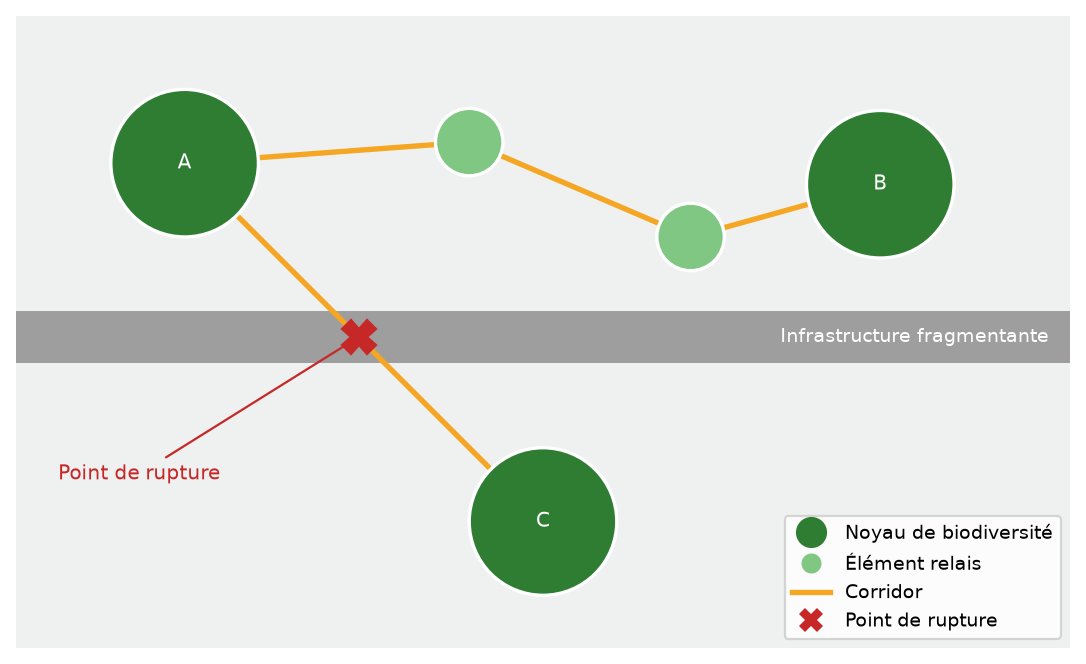
\includegraphics[width=0.98\textwidth]{figures/reseau_ecologique.png}
\caption{Schéma d'un réseau écologique : noyaux de biodiversité, corridors et espaces relais au sein de la matrice urbaine.}
\label{fig:1}
\end{figure}

\section{Le cadre réglementaire des continuités écologiques}\label{sec:1.3}

Au-delà de l'enjeu écologique, préserver ces continuités relève aussi du cadre réglementaire de l'aménagement. En France, la Trame verte et bleue (TVB), issue des lois Grenelle I \hyperref[sec:bibliographie]{(2009)} et II \hyperref[sec:bibliographie]{(2010)}, s'est traduite par des schémas régionaux de cohérence écologique (SRCE), intégrés depuis 2016 aux schémas régionaux d'aménagement (SRADDET). Les documents d'urbanisme, du schéma de cohérence territoriale (SCoT) au plan local d'urbanisme (PLU, PLUi), doivent « prendre en compte » ces continuités (article L. 371-3 du code de l'environnement), c'est-à-dire ne pas s'en écarter sans le justifier : c'est le niveau le moins contraignant de la hiérarchie des normes, en deçà de la compatibilité et de la conformité. À l'échelle européenne, la Stratégie en faveur de la biodiversité à l'horizon 2030 \hyperref[sec:bibliographie]{(Commission européenne, 2020)} fixe des objectifs, dont protéger 30 \% des terres et des mers de l'Union, planter trois milliards d'arbres et enrayer le déclin des pollinisateurs, tandis que le règlement (UE) 2024/1991 sur la restauration de la nature impose aux États des cibles contraignantes, dont l'absence de perte nette d'espaces verts urbains.

Le cadre réglementaire existe donc à plusieurs échelles, mais c'est à l'échelle locale de l'aménagement que son application reste la moins contraignante. Les cibles du règlement (UE) 2024/1991 s'imposent aux États et sont récentes : elles ne se sont pas encore traduites en obligations opposables au niveau des documents d'urbanisme, où les continuités relèvent de la seule « prise en compte », le degré le moins contraignant. Sans obligation de résultat à cette échelle, et dans des budgets locaux contraints, ces continuités mobilisent rarement des moyens dédiés. Les traduire en actes suppose des outils standardisés, reproductibles et accessibles à des gestionnaires non spécialistes, aujourd'hui rares \hyperref[sec:bibliographie]{(Vimal et al., 2012)}, et des approches de diagnostic et de suivi peu coûteuses.

Une précaution sémantique s'impose dès lors. Cette étude se rattache à ce cadre sans prétendre le remplir : elle produit des continuités écologiques potentielles, un diagnostic modélisé d'aide à la décision, et non une Trame verte et bleue réglementaire, qui suppose une identification concertée et validée sur le terrain. Le vocabulaire réglementaire de la TVB ayant été forgé pour les milieux naturels et agricoles, le groupe de travail du Cerema sur les différents types de trames lui substitue en ville des termes adaptés que cette étude reprend : le réservoir de biodiversité, qui suppose une communauté riche accomplissant tout son cycle de vie, y devient noyau de biodiversité, mieux ajusté à des espaces urbains restreints et souvent dégradés.

\section{Le projet UrbiVerde, cadre du stage}\label{sec:1.4}

Ce stage a pris place dans le projet UrbiVerde, soutenu par l'Agence Spatiale Européenne (ESA) dans le cadre de son programme Information Factory Pathfinder for Adaptation, qui finance des infrastructures transformant les données d'observation de la Terre en information utile à l'adaptation au changement climatique. UrbiVerde vise à démontrer la faisabilité d'une infrastructure opérationnelle d'observation de la Terre dédiée à la résilience urbaine : une plateforme en ligne d'aide à la décision donnant accès à des indicateurs liés aux problématiques urbaines (surchauffe et îlots de chaleur, santé de la végétation, gestion de l'eau, pollution de l'air, pollution lumineuse et sonore, accessibilité à la nature et fragmentation des continuités écologiques).

UrbiVerde réunit un consortium de quatre partenaires : CS Group (intégration de la plateforme et traitement fiable des données), Murmuration (intelligence géospatiale pilotée par l'IA et les données d'OT), le Cerema (expertise publique en aménagement durable et accès aux besoins des utilisateurs finaux) et Aerospace Valley (animation de l'écosystème et accès au marché). Le projet est soumis à deux exigences de l'ESA : réutiliser l'existant plutôt que recréer des outils, et viser une plateforme opérationnelle pérenne. Le stage s'est déroulé au sein de Murmuration, entreprise spécialisée dans l'exploitation de l'observation de la Terre et de l'intelligence artificielle au service de l'environnement et de l'adaptation au changement climatique, et a porté sur le service dédié aux continuités écologiques de la trame verte en milieu urbain. Ce cadre, appliqué d'emblée à quatre villes pilotes aux contextes contrastés, impose dès le départ que la méthode soit transposable d'un territoire à l'autre.

Dans l'architecture de la plateforme, les indicateurs sont organisés en trois niveaux de complexité croissante, chacun s'appuyant sur le précédent : l'observation de la Terre (par exemple la température de surface ou l'imagerie Sentinel) ; les services écosystémiques qui en sont dérivés (rafraîchissement urbain, bien-être, continuités écologiques) ; puis les impacts climatiques projetés. Cet outil relève du deuxième niveau, celui des services écosystémiques.

\section{État de l'art}\label{sec:1.5}

Cette section passe en revue les acquis sur lesquels s'appuie le travail : les méthodes de modélisation de la connectivité (1.5.1), les données d'occupation du sol mobilisables (1.5.2), les stratégies de sélection d'espèces (1.5.3), puis les outils existants, dont la synthèse fait ressortir le verrou auquel répond ce travail (1.5.4). Modéliser la connectivité écologique mobilise en effet un corpus méthodologique établi, dont les briques sont connues mais rarement assemblées en une chaîne unique.

\subsection{De l'habitat aux corridors : méthodes et controverses}\label{sec:1.5.1}

Modéliser la connectivité mobilise plusieurs familles de méthodes (\hyperref[fig:2]{Figure 2}), de l'identification des habitats au tracé des corridors, que les études combinent rarement toutes. Chacune dispose aujourd'hui de méthodes établies, mais chacune porte une limite reconnue par ceux qui l'emploient ; l'accumulation de ces limites, plus qu'une faiblesse isolée, dessine le verrou auquel ce travail répond. Les méthodes sont ici passées en revue ; les choix retenus pour la chaîne sont exposés au \hyperref[chap:2]{chapitre 2}.

\begin{figure}[H]
\centering
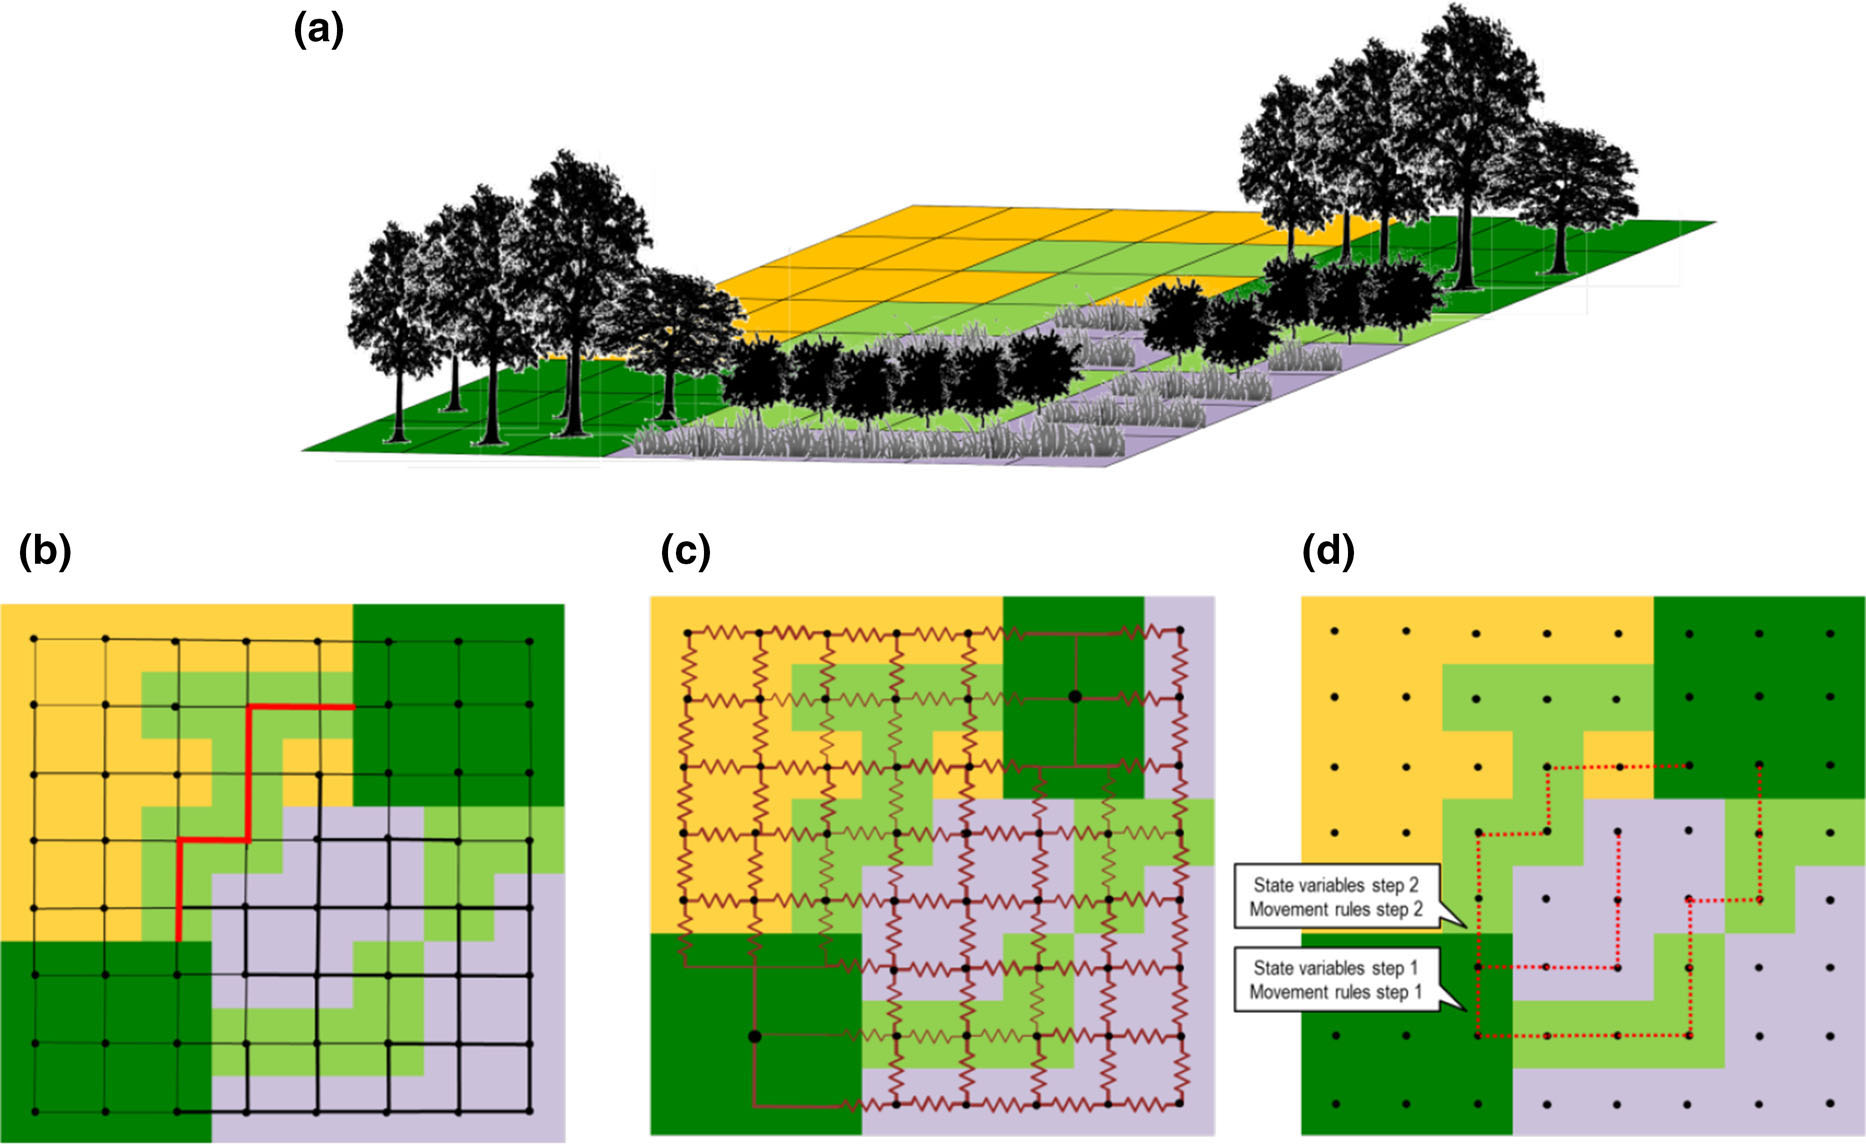
\includegraphics[width=0.98\textwidth]{figures/diniz_connectivity_models.png}
\caption{Surface de résistance au déplacement et principales familles de modèles de connectivité : le paysage comme surface de résistance (a), le modèle de moindre coût (b), la théorie des circuits (c) et les modèles individus-centrés (d). (d'après Diniz et al., 2020)}
\label{fig:2}
\end{figure}

La configuration spatiale de l'habitat est le plus souvent décrite par analyse morphologique (Morphological Spatial Pattern Analysis, MSPA), qui classe chaque pixel d'une couche binaire habitat / non-habitat en catégories morphologiques (coeur, îlot, perforation, lisière, boucle, pont, branche) au moyen d'opérations de morphologie mathématique \hyperref[sec:bibliographie]{(Soille \& Vogt, 2009 ; Vogt et al., 2007)}. Elle sépare les grandes taches des petits éléments à partir d'un unique paramètre de largeur de bord. Sa limite est que ce paramètre n'a pas de valeur canonique : les sorties dépendent fortement de l'échelle et de la binarisation retenues \hyperref[sec:bibliographie]{(Ostapowicz et al., 2008)}, au point que les logiciels de référence documentent ces réglages comme des choix d'utilisateur, non comme des standards \hyperref[sec:bibliographie]{(Vogt \& Riitters, 2017)}. L'identification même de l'habitat est donc déjà une décision de modélisation.

Le déplacement entre taches est ensuite représenté par une surface de résistance, qui attribue à chaque classe d'occupation du sol un coût de franchissement \hyperref[sec:bibliographie]{(Adriaensen et al., 2003)}. C'est l'entrée la plus déterminante et la moins contrainte de toute la chaîne : la revue de Zeller et al. \hyperref[sec:bibliographie]{(2012)}, sur quatre-vingt-seize travaux, montre que ces coûts sont majoritairement fixés à dire d'expert et rarement calibrés, d'où des recommandations divergentes d'une étude à l'autre \hyperref[sec:bibliographie]{(Beier et al., 2008)}. Les calibrations empiriques, par génétique du paysage \hyperref[sec:bibliographie]{(Cushman et al., 2006)} ou analyse de sensibilité \hyperref[sec:bibliographie]{(Spear et al., 2010)}, restent coûteuses et rares ; et la favorabilité d'habitat, souvent employée comme substitut, prédit mal la résistance au déplacement \hyperref[sec:bibliographie]{(Stevenson-Holt et al., 2014)}. La matrice concentre ainsi l'essentiel de l'incertitude du modèle.

À l'échelle du réseau, le paysage est modélisé comme un graphe dont les noeuds sont les taches et les liens les connexions possibles, pondérées par une probabilité de déplacement décroissant avec la distance \hyperref[sec:bibliographie]{(Urban \& Keitt, 2001 ; Fall et al., 2007 ; Urban et al., 2009)}. La topologie du réseau n'est toutefois pas donnée : le choix de la règle de liaison, du graphe le plus parcimonieux (arbre couvrant minimal) aux plus denses (k plus proches voisins), modifie sensiblement le résultat, sans qu'un consensus se dégage \hyperref[sec:bibliographie]{(Minor \& Urban, 2008 ; Galpern et al., 2011)}. Le choix de la topologie pèse donc directement sur la connectivité mesurée.

De cette représentation dérivent les principaux indices de disponibilité d'habitat : l'Integral Index of Connectivity (IIC), fondé sur un lien binaire \hyperref[sec:bibliographie]{(Pascual-Hortal \& Saura, 2006)}, puis la Probability of Connectivity (PC), qui le généralise à une probabilité continue de déplacement et s'interprète comme la probabilité que deux points tirés au hasard tombent dans des habitats mutuellement accessibles \hyperref[sec:bibliographie]{(Saura \& Pascual-Hortal, 2007)}. La PC se décline en une surface équivalente connectée exprimant la connectivité en unité de surface \hyperref[sec:bibliographie]{(Saura et al., 2011)} et se décompose, au retrait d'un élément, en contributions distinguant sa surface propre, le flux qui transite par lui et son rôle de relais \hyperref[sec:bibliographie]{(Saura \& Rubio, 2010)} ; des mesures de centralité de graphe, dont l'intermédiarité, hiérarchisent en complément les taches et les liens selon le flux qu'ils portent \hyperref[sec:bibliographie]{(Estrada \& Bodin, 2008)}. Ces indices fournissent une hiérarchisation fine, mais tous dépendent étroitement du paramètre de dispersion retenu \hyperref[sec:bibliographie]{(Rayfield et al., 2011 ; Urban et al., 2009)}.

Le tracé des corridors oppose deux familles de méthodes. Le chemin de moindre coût \hyperref[sec:bibliographie]{(algorithme de Dijkstra ; Adriaensen et al., 2003)} identifie le trajet optimal sur la surface de résistance (\hyperref[fig:3]{Figure 3}) et a été appliqué à la planification urbaine \hyperref[sec:bibliographie]{(Balbi et al., 2019)}. Un tel tracé reste néanmoins un trait de largeur nulle : le chemin optimal en coût n'est pas l'emprise optimale d'un corridor \hyperref[sec:bibliographie]{(Pinto \& Keitt, 2009 ; Shirabe, 2018 ; Etherington, 2016)}, et sa validité dépend de valeurs de résistance rarement confrontées au mouvement réel \hyperref[sec:bibliographie]{(Sawyer et al., 2011)}. La théorie des circuits \hyperref[sec:bibliographie]{(McRae et al., 2008)} restitue à l'inverse un gradient de perméabilité intégrant toutes les trajectoires \hyperref[sec:bibliographie]{(Koen et al., 2014)}. L'opposition entre un déplacement optimal et une marche aléatoire est cependant une simplification : le cadre des chemins aléatoires pondérés les unifie, et les validations sur données de mouvement situent le déplacement réel entre ces deux extrêmes \hyperref[sec:bibliographie]{(Panzacchi et al., 2016 ; Goicolea et al., 2021)}. Là encore, le tracé obtenu traduit une hypothèse de comportement, non une trajectoire observée.

\begin{figure}[H]
\centering
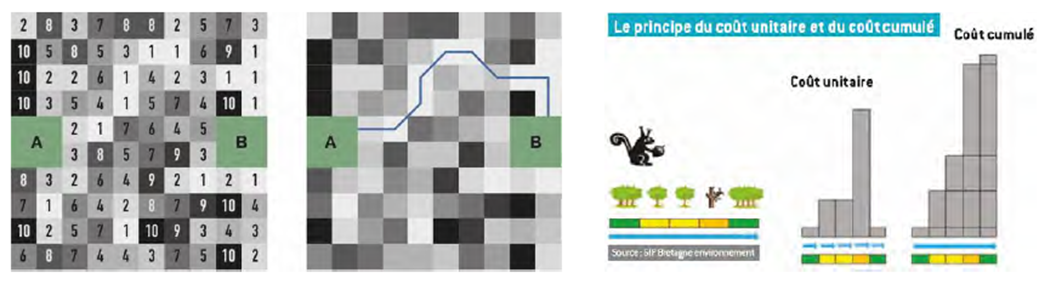
\includegraphics[width=0.98\textwidth]{figures/lcp_principe.png}
\caption{Principe du chemin de moindre coût sur une surface de friction (à gauche) et du coût cumulé le long du trajet (à droite). (source : GIP Bretagne environnement, via MitiConnect)}
\label{fig:3}
\end{figure}

Une famille plus synthétique quantifie enfin directement la fragmentation par la taille de maille effective, fondée sur la probabilité que deux points tirés au hasard appartiennent à la même zone connectée \hyperref[sec:bibliographie]{(Jaeger, 2000 ; Spanowicz \& Jaeger, 2019)}. Cette mesure alimente notamment le City Biodiversity Index, ou indice de Singapour, cadre d'auto-évaluation normalisé endossé par la Convention sur la diversité biologique et adopté par de nombreuses villes : vingt-trois indicateurs notés de 0 à 4 (score maximal de 92), répartis en trois volets, la biodiversité native, les services écosystémiques et la gouvernance \hyperref[sec:bibliographie]{(Secrétariat de la CDB, 2021)}. La connectivité y figure comme un unique indicateur du volet biodiversité native, quantifié par la taille de maille effective \hyperref[sec:bibliographie]{(Deslauriers et al., 2018)}, indicateur ensuite décliné en outil de planification urbaine par groupes d'espèces \hyperref[sec:bibliographie]{(Kirk et al., 2023)}. L'indice offre ainsi un étalon comparable d'une ville à l'autre, mais réduit la connectivité à une note agrégée, sans localiser où elle est en jeu, et repose sur une connectivité binaire, deux taches étant reliées ou non, là où les approches par graphe, moindre coût ou circuit autorisent un gradient de déplacement.

En somme, aucune de ces méthodes n'est universelle : le choix dépend de l'objectif et de l'échelle, et les approches structurelles, fonctionnelles et de réseau éclairent chacune une facette différente de la connectivité \hyperref[sec:bibliographie]{(Pechanec et al., 2025)}. Surtout, trois limites traversent l'ensemble et se cumulent : ces méthodes reposent sur des paramètres à dire d'expert rarement calibrés, elles sont très sensibles à ce paramétrage, et elles sont peu confrontées au mouvement réel. C'est le premier des éléments qui constituent le verrou, complété par les sections suivantes.

\subsection{Données d'occupation du sol pour la connectivité}\label{sec:1.5.2}

Une chaîne de connectivité requiert une carte d'occupation du sol distinguant les habitats pertinents pour les espèces (boisements, formations arbustives, prairies) de la matrice urbaine. L'observation de la Terre fournit cette couche avec une couverture exhaustive et homogène, une mise à jour régulière et un traitement reproductible, là où les inventaires de terrain sont coûteux et ponctuels.

Deux voies coexistent, aux compromis opposés. La première produit une classification sur mesure à partir d'images satellitaires, par méthodes classiques \hyperref[sec:bibliographie]{(classification orientée objet ; Blaschke, 2010)} ou par segmentation sémantique profonde, éventuellement sur séries temporelles \hyperref[sec:bibliographie]{(Wang et al., 2022 ; Inglada et al., 2017)}. Performante, elle exige des données annotées, un ré-entraînement propre à chaque contexte, et reste exposée au glissement de domaine, sa performance chutant lorsque le modèle est transféré à une autre ville ou un autre capteur \hyperref[sec:bibliographie]{(Tuia et al., 2016)} : elle est donc lourde à transposer. La seconde réutilise des produits prêts à l'emploi, soit nationaux et fins (en France l'OCS GE, la CoSIA, la BD TOPO, le RPG), mais bornés à un pays et donc incompatibles avec une chaîne internationale, soit mondiaux et libres \hyperref[sec:bibliographie]{(ESA WorldCover, Dynamic World ; Zanaga et al., 2021 ; Brown et al., 2022)}, disponibles partout au prix d'une résolution de 10 m trop grossière pour les éléments linéaires fins et les petits relais \hyperref[sec:bibliographie]{(Radoux et al., 2016)}.

Ces produits mondiaux ont une limite documentée : leur précision globale, de 65 à 84 \% selon le produit et la validation, ne s'ordonne pas de façon stable entre eux et se dégrade dans les paysages hétérogènes comme la ville \hyperref[sec:bibliographie]{(Venter et al., 2022 ; Xu et al., 2024)}. Des travaux récents montrent qu'employés seuls, ils restent insuffisants pour la connectivité urbaine, une carte fine multi-source (par exemple vingt-trois classes à 10 m, précision d'environ 82 \%) s'avérant nécessaire \hyperref[sec:bibliographie]{(Pundsack et al., 2025)}. OpenStreetMap, base collaborative libre, comble une part de ce manque en apportant les objets absents ou trop grossiers des produits mondiaux (réseaux routiers et ferrés, bâti fin, surfaces en eau, espaces verts) ; sa complétude est bonne en milieu urbain, mais la finesse de son étiquetage varie d'une ville et d'un pays à l'autre \hyperref[sec:bibliographie]{(Barrington-Leigh \& Millard-Ball, 2017)}.

Aucune source ne réunit ainsi finesse, couverture mondiale, gratuité et reproductibilité : la voie transposable et sans coût, celle des produits mondiaux libres complétés par OpenStreetMap, se paie d'une résolution grossière. C'est le deuxième élément du verrou.

\subsection{Représenter la faune : espèces focales, guildes et profils écologiques}\label{sec:1.5.3}

Paramétrer un modèle de connectivité par espèce suppose des données de distribution et de mouvement souvent indisponibles en ville. Les bases d'occurrence comme le GBIF (Global Biodiversity Information Facility) ou l'INPN (Inventaire national du patrimoine naturel) reposent largement sur des observations opportunistes issues des sciences participatives : l'effort d'observation y est inégal, concentré sur les zones accessibles et les espèces les plus visibles (oiseaux notamment), au détriment des taxons discrets ou nocturnes et des secteurs peu fréquentés. Ce biais d'échantillonnage \hyperref[sec:bibliographie]{(Isaac et al., 2014)} fait que la donnée reflète autant la répartition des observateurs que celle des espèces ; s'y ajoutent une couverture inégale d'un territoire à l'autre et la rareté des données empiriques de déplacement \hyperref[sec:bibliographie]{(constat également formulé par Kirk et al., 2023)}.

Faute de données par espèce, plusieurs façons de représenter la faune coexistent. L'approche par espèce focale retient une espèce dont les exigences de déplacement et d'habitat dimensionnent le réseau \hyperref[sec:bibliographie]{(Lambeck, 1997)} : elle rend les choix explicites mais dépend d'une seule espèce. La désigner comme parapluie, phare ou indicatrice suppose qu'elle représente les autres, hypothèse que les tests empiriques ne confirment guère \hyperref[sec:bibliographie]{(une espèce-substitut unique ne fait souvent pas mieux qu'un choix au hasard ; Andelman \& Fagan, 2000)}, la fiabilité des substituts n'étant établie que sous conditions, à échelle large, en multi-espèces et à un niveau taxonomique élevé \hyperref[sec:bibliographie]{(Tälle et al., 2023)}. De là plusieurs voies multi-espèces : un jeu restreint d'espèces focales complémentaires aux exigences contrastées \hyperref[sec:bibliographie]{(Meurant et al., 2018)} ; des guildes ou groupes fonctionnels rassemblant les espèces par comportement de dispersion, ce qui révèle des réponses contrastées à la fragmentation qu'une espèce unique masquerait \hyperref[sec:bibliographie]{(Lechner et al., 2017)} ; ou des profils écologiques composites, aussi appelés espèces génériques, virtuelles ou « chimères », construits à partir des niches et des traits de plusieurs espèces : ils approchent un grand nombre d'espèces réelles sans exiger de données propres à chacune \hyperref[sec:bibliographie]{(Watts et al., 2010 ; Prima et al., 2024)}. En contexte urbain, une évaluation multi-taxons peut même modifier la décision d'aménagement, par exemple entre renaturaliser une grande zone ou plusieurs petites \hyperref[sec:bibliographie]{(Gelmi-Candusso et al., 2025)}.

En France, la Trame verte et bleue structure les continuités en sous-trames, chacune rassemblant l'ensemble des espaces d'un même type de milieu (boisé, arbustif, herbacé, humide) et le réseau qu'ils forment \hyperref[sec:bibliographie]{(Sordello, 2017)}. Une sous-trame est une entité de milieu, à distinguer du cortège, qui désigne l'assemblage d'espèces associé à ce milieu (espèces aux exigences écologiques proches, susceptibles d'y coexister). Cette entrée par milieu, privilégiée par les documents de planification pour sa lisibilité et son ancrage réglementaire, suppose toutefois une occupation du sol assez fine pour séparer les strates de végétation ; le Cerema Dter Sud-Ouest \hyperref[sec:bibliographie]{(2025)} en donne une déclinaison opérationnelle, en moyennant les frictions des espèces d'un même cortège.

Chacune établit un compromis différent entre exigence en données et réalisme écologique : le choix dépend donc des données disponibles et de l'objectif \hyperref[sec:bibliographie]{(Tälle et al., 2023)}.

\subsection{Outils existants et verrou opérationnel}\label{sec:1.5.4}

Plusieurs logiciels mettent en oeuvre ces méthodes : Graphab pour les graphes paysagers \hyperref[sec:bibliographie]{(Foltête et al., 2012)}, Conefor pour les indices de connectivité \hyperref[sec:bibliographie]{(Saura \& Torné, 2009)}, Circuitscape pour la théorie des circuits \hyperref[sec:bibliographie]{(McRae et al., 2008)}, ou des extensions QGIS comme Biodispersal (M. Chailloux, UMR TETIS), employée par le Cerema, et MitiConnect (INRAE), qui enchaîne ces étapes autour de la séquence Éviter-Réduire-Compenser en s'appuyant sur Graphab. La démarche de Kirk et al. \hyperref[sec:bibliographie]{(2023)} s'appuie de même sur un enchaînement manuel d'opérations sous QGIS complété par un tableur.

Ces outils partagent trois traits qui bornent leur usage opérationnel à grande échelle : ils requièrent une expertise en système d'information géographique (SIG) et une préparation manuelle des couches ; ils sont le plus souvent appliqués au cas par cas sur des données fines locales, donc peu transposables d'un territoire à l'autre ; et ils restituent rarement des résultats directement exploitables par un gestionnaire non spécialiste. Ce déficit n'est pas que technique : le bilan de deux cent soixante-trois plans de connectivité de Keeley et al. \hyperref[sec:bibliographie]{(2019)} montre que leur adoption ne dépend ni du modèle ni des données employés, mais de la transparence, de la reproductibilité de la procédure et de son portage institutionnel ; et la connectivité demeure un concept encore mal traduit en objectifs opérationnels \hyperref[sec:bibliographie]{(Beger et al., 2022)}. La reproductibilité n'est donc pas une simple exigence de méthode, elle conditionne l'usage.

Deux travaux publiés situent ce constat par contraste. Liu et al. \hyperref[sec:bibliographie]{(2022)} déploient la chaîne complète (analyse morphologique, métriques de graphe, moindre coût, théorie des circuits) sur Pékin, mais à l'échelle régionale (réservoirs d'au moins 50 ha, dispersion de l'ordre de 20 à 25 km) et indépendamment des espèces, par assemblage manuel d'outils de bureau ; leur propre conclusion appelle à une différenciation multi-espèces. Kirk et al. \hyperref[sec:bibliographie]{(2023)} opèrent à l'inverse à l'échelle intra-urbaine, par groupes fonctionnels et de façon reproductible autour de scénarios avant et après, mais restent sur une connectivité binaire et un enchaînement manuel.

Ces limites convergent ici. Les méthodes sont puissantes mais reposent sur des paramètres experts peu calibrés et rarement confrontés au mouvement réel (1.5.1) ; la seule voie de données transposable et libre se paie d'une résolution grossière (1.5.2) ; et les outils qui les mettent en oeuvre exigent une expertise, se transposent mal et ne produisent pas de sortie directement actionnable. Ce qu'aucun ne réunit, c'est l'automatisation, l'appui sur des données ouvertes, la reproductibilité sur des contextes contrastés et une sortie directement exploitable pour la décision. Ce travail vise précisément cette combinaison.

\section{Problématique, objectifs et plan}\label{sec:1.6}

En réponse à ce verrou, la présente étude construit et teste une preuve de concept : une chaîne de traitement qui identifie les continuités écologiques urbaines potentielles à partir de la seule observation de la Terre et de données ouvertes. Ce choix de données répond directement aux limites relevées plus haut, en visant une chaîne homogène, gratuite et transposable d'un territoire à l'autre plutôt qu'un outil calibré localement. Les choix de données, de profils écologiques et de méthode qui en découlent sont exposés au \hyperref[chap:2]{chapitre 2}.

De ce positionnement découle la problématique du stage :

\begin{quote}
\textbf{Comment construire un outil de connectivité écologique urbaine, piloté par l'observation de la Terre et des données ouvertes, reproductible sur des territoires aux contextes bioclimatiques contrastés, et produisant des recommandations spatiales exploitables par les gestionnaires des infrastructures vertes ?}
\end{quote}

Pour y répondre, le travail poursuit les objectifs suivants :

1. concevoir une chaîne de traitement de bout en bout, depuis les données ouvertes (WorldCover et OpenStreetMap, OSM) jusqu'aux composantes des continuités écologiques potentielles (noyaux de biodiversité, corridors, points de rupture, surfaces de dispersion) ; 2. rester pertinent sur des territoires aux faunes contrastées sans calibrage local, en représentant plusieurs profils de déplacement plutôt qu'une espèce unique ; 3. implémenter l'ensemble intégralement en Python, sans recourir aux logiciels spécialisés existants (Biodispersal sous QGIS, Graphab), pour obtenir un pipeline automatisable, reproductible et transposable ; 4. restituer les résultats dans un tableau de bord interactif d'aide à la décision, destiné aux aménageurs ; 5. démontrer la transposabilité de la chaîne sur des contextes bioclimatiques et urbains contrastés.

Le présent chapitre a posé le contexte, l'état de l'art et la problématique. Le \hyperref[chap:2]{chapitre 2} décrit les données et la méthode ; le \hyperref[chap:3]{chapitre 3} présente les résultats sur les six territoires ; le \hyperref[chap:4]{chapitre 4} les discute et les confronte à la méthode du Cerema ; le \hyperref[chap:5]{chapitre 5} conclut ; le \hyperref[chap:6]{chapitre 6} propose un retour d'expérience sur le déroulement du stage.

\chapter{Données et méthodes}\label{chap:2}

Ce chapitre décrit la chaîne de traitement de bout en bout : les territoires d'étude (\hyperref[sec:2.1]{§2.1}), les données ouvertes qui l'alimentent (\hyperref[sec:2.2]{§2.2}), les profils écologiques et leur calibration (\hyperref[sec:2.3]{§2.3}), les étapes de calcul des continuités (\hyperref[sec:2.4]{§2.4}), l'implémentation logicielle et le contrôle automatisé des sorties (\hyperref[sec:2.5]{§2.5}) et leur restitution dans un tableau de bord (\hyperref[sec:2.6]{§2.6}).

\section{Territoires d'étude}\label{sec:2.1}

La chaîne a été appliquée à des territoires aux contextes bioclimatiques volontairement contrastés (\hyperref[fig:4]{Figure 4}). Quatre villes pilotes du projet UrbiVerde ont servi de terrains de développement : La Roche-sur-Yon (agglomération, façade atlantique), Nancy (métropole du Grand Nancy, climat continental du nord-est), Perpignan (commune, climat méditerranéen) et Kourou, en Guyane (climat équatorial). Deux territoires supplémentaires ont servi à contrôler et valider les sorties : Toulouse (métropole), retenue comme cas de contrôle visuel, en raison d'une bonne connaissance de terrain, et l'agglomération de La Rochelle, territoire de la méthode Cerema Dter Sud-Ouest à laquelle ce travail se compare et dont il emprunte une partie de la calibration (détaillée en \hyperref[sec:2.3]{§2.3}).

\begin{figure}[H]
\centering
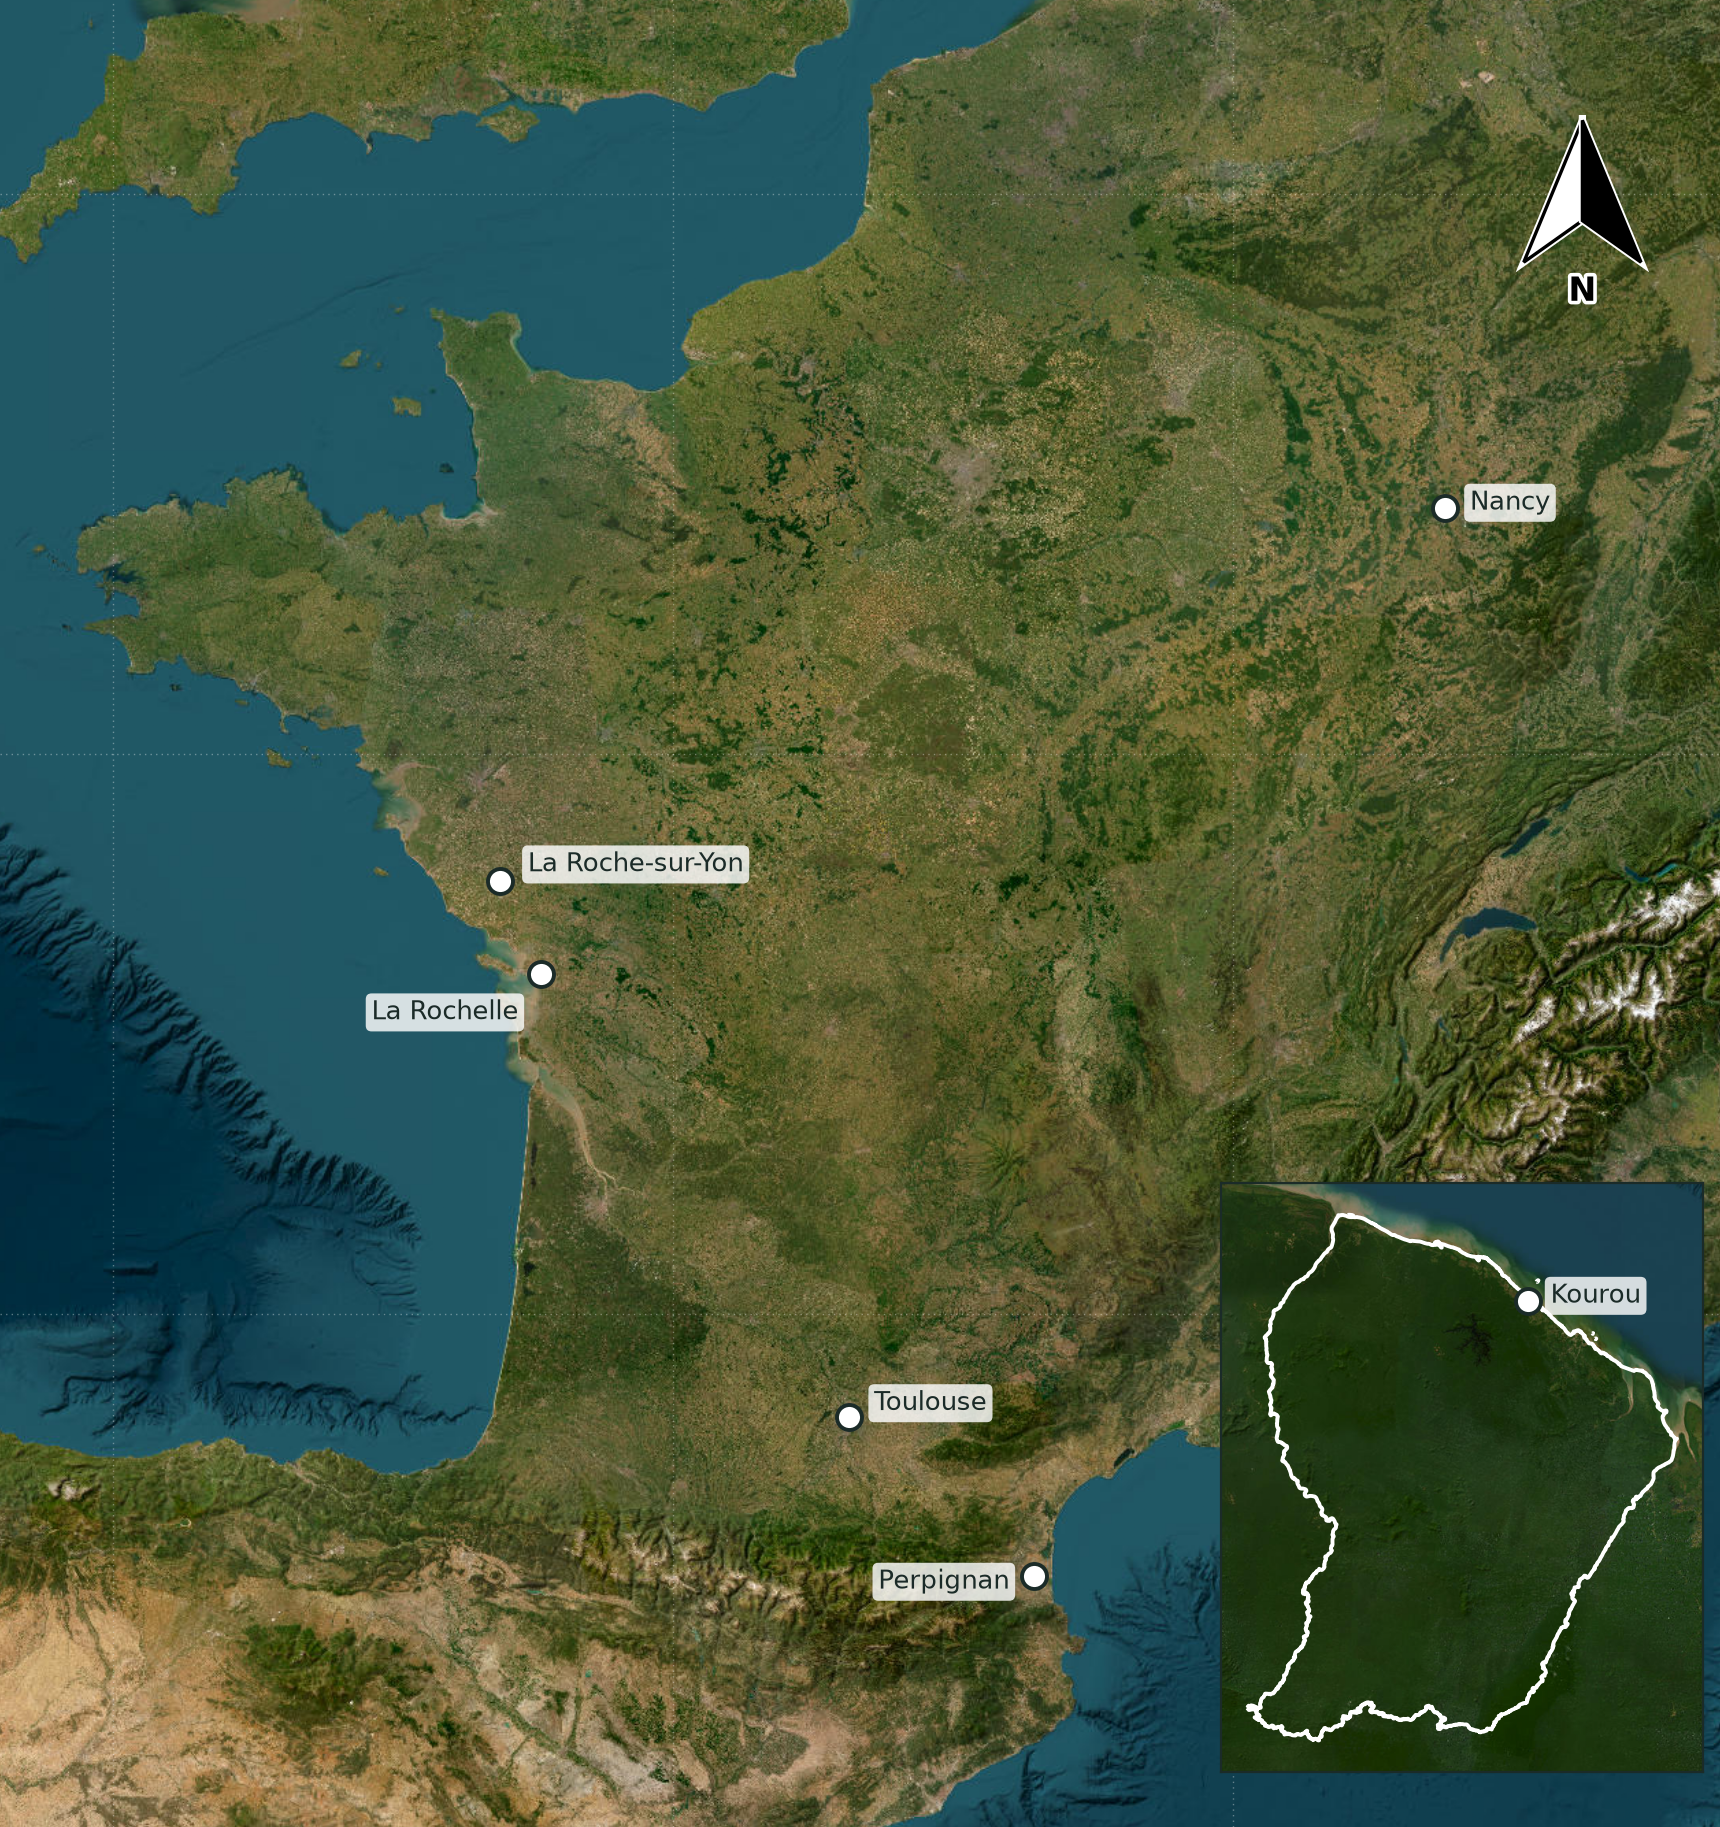
\includegraphics[width=0.98\textwidth]{figures/localisation_territoires_osm.png}
\caption{Localisation des six territoires d'étude. (fond de carte OpenStreetMap, 2026)}
\label{fig:4}
\end{figure}

Pour chaque territoire, la zone d'étude est définie à partir de ses limites administratives, Kourou faisant exception avec une emprise rectangulaire, sa limite communale étant trop restreinte pour englober les espaces périurbains pertinents. Elle est ensuite élargie par un tampon égal à deux fois la plus grande distance de dispersion considérée (soit 6 km). Ce tampon corrige l'effet de bord, une frontière de carte artificielle se comportant comme une barrière qui sous-estime la connectivité des taches périphériques \hyperref[sec:bibliographie]{(Koen et al., 2010, 2014)} : un corridor peut s'appuyer sur une tache d'habitat située juste en dehors de la limite administrative, qui serait ignorée si l'analyse s'arrêtait à cette limite. Les habitats du tampon servent ainsi de relais au calcul, mais seules les composantes situées dans la zone d'étude stricte sont comptabilisées dans les résultats.

La superficie de la zone d'étude, tampon compris, varie fortement d'un territoire à l'autre, de 68 km² à Perpignan à 502 km² à La Roche-sur-Yon (Tableau 1). Cette différence d'emprise tient à la taille des limites administratives retenues ; il faut en tenir compte pour lire en valeur absolue les surfaces d'habitat et la surface connectée équivalente (définies en \hyperref[sec:2.4]{§2.4}), qui croissent mécaniquement avec l'étendue du territoire. La part d'habitat connecté, normalisée, reste elle comparable d'un site à l'autre.

\begin{table}[H]
\centering
\caption{Les six territoires d'étude, leur statut et la superficie de la zone d'étude (tampon de 6 km inclus).}
\begin{tabularx}{\textwidth}{>{\raggedright\arraybackslash}X >{\raggedright\arraybackslash}X >{\raggedright\arraybackslash}X >{\raggedright\arraybackslash}X}
\toprule
\textbf{Territoire} & \textbf{Statut} & \textbf{Contexte bioclimatique} & \textbf{Zone d'étude (km², tampon inclus)} \\
\midrule
La Roche-sur-Yon & pilote & atlantique & 502 \\
Nancy & pilote & continental (nord-est) & 143 \\
Perpignan & pilote & méditerranéen & 68 \\
Kourou (Guyane) & pilote & équatorial & 123 \\
Toulouse & contrôle visuel & océanique à influence méditerranéenne & 461 \\
La Rochelle & validation (comparaison Cerema) & atlantique & 331 \\
\bottomrule
\end{tabularx}
\end{table}

Kourou occupe un statut à part. C'est un territoire pilote d'UrbiVerde, mais la connectivité écologique n'y est pas l'enjeu le plus pertinent, d'autres indicateurs de la plateforme y faisant davantage sens ; et les profils écologiques, calibrés sur des espèces de métropole, n'y représentent pas la faune locale. Il sert donc ici de test de transposabilité de la chaîne à un biome très différent, non de diagnostic écologique directement exploitable (réserve développée en section 4.2).

\section{Données et acquisition}\label{sec:2.2}

La chaîne part d'une couche d'occupation du sol, qui attribue à chaque pixel une classe de milieu (arbres, prairies, bâti, eau\ldots{}) : c'est d'elle que sont dérivés l'habitat propre à chaque profil écologique et la résistance de la matrice au déplacement. Cette couche repose sur le produit mondial ESA WorldCover \hyperref[sec:bibliographie]{(version 200, résolution 10 m ; Zanaga et al., 2021)}, dérivé des imageries Sentinel-1 et Sentinel-2 et récupéré via Google Earth Engine sur l'emprise tamponnée. WorldCover distingue onze classes, parmi lesquelles les arbres (code 10), les arbustes (20), les prairies (30), les cultures (40), les surfaces bâties et imperméabilisées (50), les sols nus (60), l'eau (80), les zones humides (90) et les mangroves (95).

Ce produit ne représente toutefois pas les infrastructures fragmentantes (routes, voies ferrées) avec la finesse requise, alors qu'elles constituent les principales barrières au déplacement terrestre. Celles-ci sont donc ajoutées à partir des données ouvertes d'OpenStreetMap, dont la complétude du réseau routier est bonne en milieu urbain \hyperref[sec:bibliographie]{(Barrington-Leigh \& Millard-Ball, 2017)} : réseaux routiers, voies ferrées, emprises bâties et surfaces en eau, ainsi que certaines surfaces artificialisées gérées (aéroports, stades). Ces éléments sont rastérisés et brûlés par-dessus le WorldCover selon un ordre de priorité fixe (détaillé en \hyperref[annexe:A]{annexe A}), ce qui ajoute aux codes WorldCover des codes spécifiques d'occupation artificialisée : emprises bâties (51), routes principales et autoroutes (52), routes secondaires (53), chemins (54) et voies ferrées (55) ; l'occupation du sol enrichie est illustrée \hyperref[fig:5]{Figure 5} pour Toulouse. Toutes les analyses sont menées dans la projection métrique locale (UTM) propre à chaque territoire, les distances et surfaces étant exprimées en mètres, mètres carrés et hectares.

\begin{figure}[H]
\centering
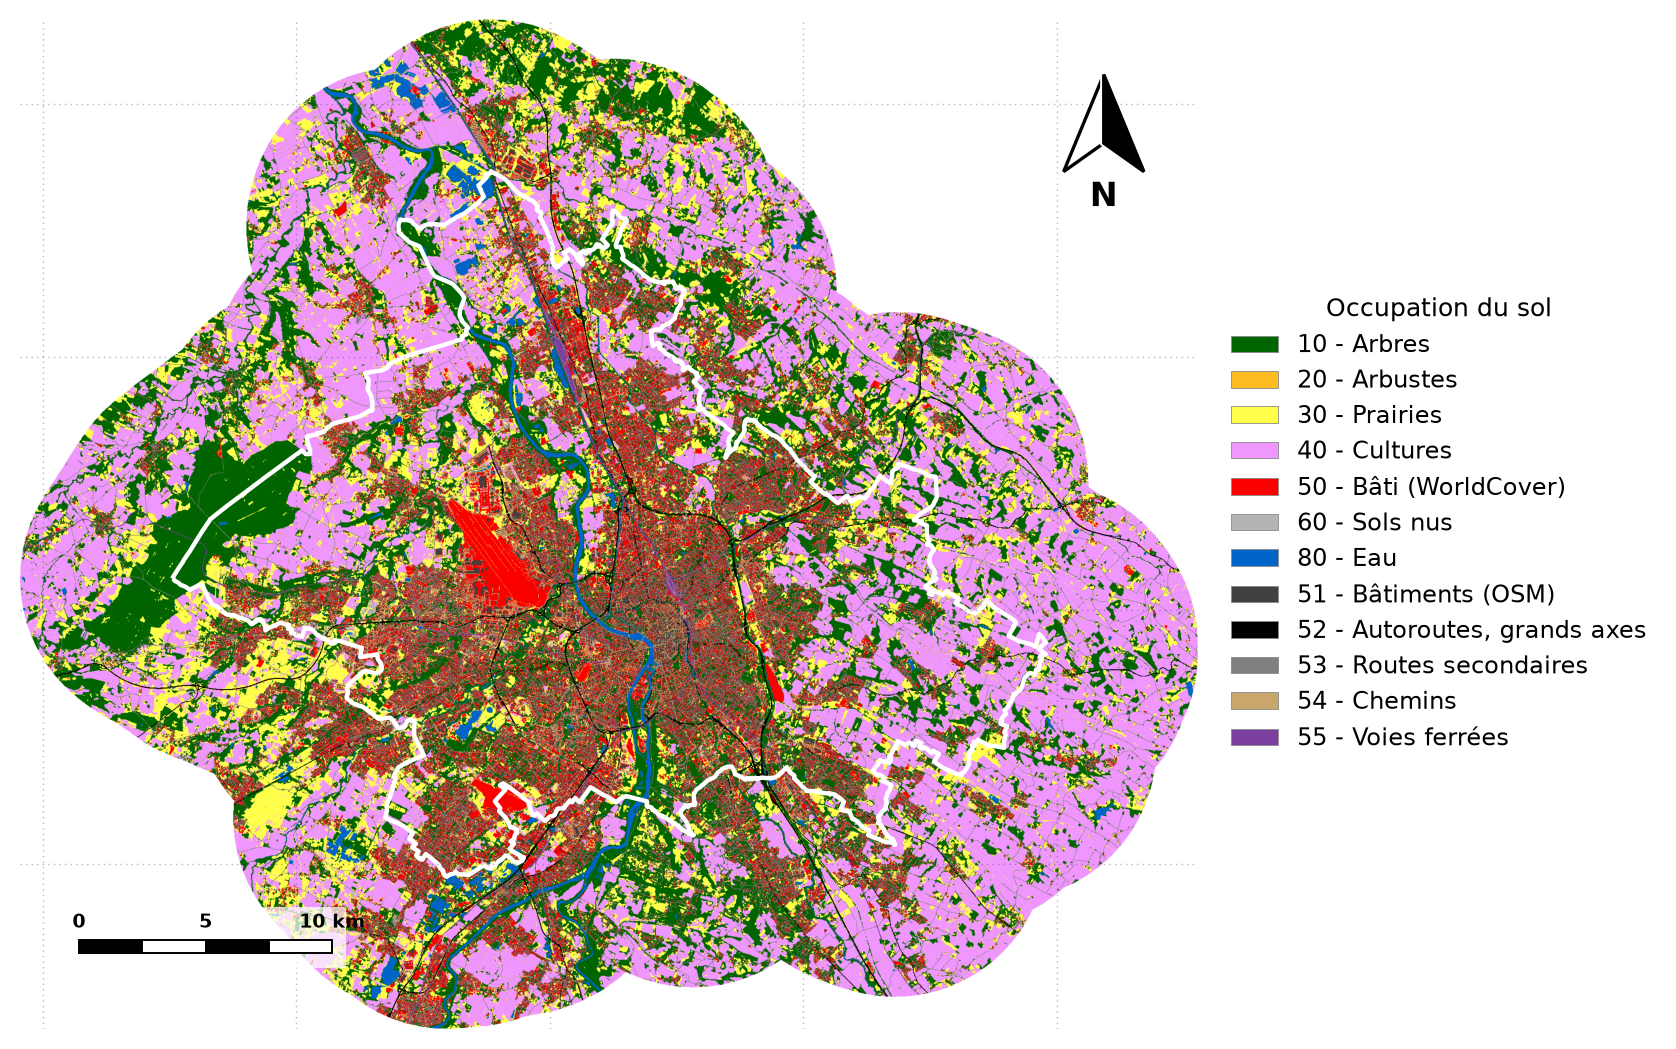
\includegraphics[width=0.98\textwidth]{figures/landcover_toulouse.png}
\caption{Occupation du sol enrichie de Toulouse. (d'après ESA WorldCover et OpenStreetMap, 2026)}
\label{fig:5}
\end{figure}

Le recours à des données ouvertes et mondiales (WorldCover, OpenStreetMap) plutôt qu'aux référentiels nationaux plus fins disponibles en France (OCS GE, CoSIA) répond à l'objectif de reproductibilité de l'outil et rejoint la priorité « réutiliser l'existant » fixée par l'ESA : une donnée mondiale, gratuite et homogène garantit une chaîne identique et comparable d'un territoire à l'autre, là où un référentiel national, même de meilleure qualité, reste limité à la France et interdit une transposition mondiale. La contrepartie, assumée, est une perte de détail : la résolution de 10 m est grossière pour les éléments linéaires fins et ne capte que les grandes surfaces d'eau \hyperref[sec:bibliographie]{(Radoux et al., 2016)}. Une itération future sur un territoire français exigeant plus de précision pourrait réalimenter la chaîne avec un produit comme Green Urban Sat (GUS, Cerema), qui cartographie les strates de végétation urbaine à partir d'imagerie Pléiades [à sourcer : documentation GUS, Cerema], au prix d'une adaptation des classes d'occupation du sol. Ce compromis précision/reproductibilité est discuté au \hyperref[chap:4]{chapitre 4}.

Une correction de qualité est appliquée en amont de la chaîne : WorldCover classe la pelouse rase des aérodromes et des stades en prairie, que les profils écologiques de milieux ouverts compteraient à tort comme habitat ; ces emprises, repérées par leurs tags OpenStreetMap, sont gravées en surface imperméable pour les exclure.

\section{Profils écologiques et calibration}\label{sec:2.3}

La chaîne repose sur deux choix liés : raisonner par profils écologiques plutôt que par une espèce focale unique, et calibrer leurs paramètres sur une méthode de référence, celle du Cerema, direction territoriale Sud-Ouest (Dter Sud-Ouest), sur les continuités écologiques urbaines de la Communauté d'agglomération de La Rochelle \hyperref[sec:bibliographie]{(Cerema Dter Sud-Ouest, 2025)}.

Raisonner par profil restitue les besoins de continuité propres à chaque capacité de déplacement, qu'une entrée par espèce focale unique laisserait invisibles. L'outil s'inscrit dans la lignée des approches par espèces focales génériques et par groupes fonctionnels \hyperref[sec:bibliographie]{(Lambeck, 1997 ; Watts et al., 2010 ; Meurant et al., 2018 ; Kirk et al., 2023 ; Albert \& Chaurant, 2018)} : chaque profil écologique (écoprofil) est un syndrome écologique nommé d'après une espèce repère ubiquiste en France métropolitaine, et défini par ses codes d'habitat, sa distance caractéristique de dispersion d$_{0}$ et ses coefficients de friction par classe d'occupation du sol ; ces traits sont documentés pour les espèces repères retenues \hyperref[sec:bibliographie]{(Morris, 1988 ; Huijser \& Bergers, 2000 ; Avon et al., 2014 ; Tarabon et al., 2019)} et rassemblés en vue de leur application aux corridors \hyperref[sec:bibliographie]{(Quiblier, 2007)}. La notion d'écoprofil remonte à Vos et al. \hyperref[sec:bibliographie]{(2001)}, qui définissent un profil par ses exigences d'habitat et sa capacité de déplacement ; ces deux critères sont repris ici, mais non le troisième qu'ils y ajoutent, une surface minimale d'habitat. Quatre profils écologiques sont retenus (Tableau 2).

\begin{table}[H]
\centering
\caption{Caractéristiques des quatre profils écologiques (espèce repère, distance de dispersion, habitat, obstacles infranchissables). (d'après Cerema Dter Sud-Ouest, 2025)}
\begin{tabularx}{\textwidth}{>{\raggedright\arraybackslash}X >{\raggedright\arraybackslash}X >{\raggedright\arraybackslash}X >{\raggedright\arraybackslash}X >{\raggedright\arraybackslash}X}
\toprule
\textbf{Profil écologique} & \textbf{Espèce repère} & \textbf{d$_{0}$ (m)} & \textbf{Habitat} & \textbf{Obstacles infranchissables} \\
\midrule
Petit mammifère terrestre & Hérisson d'Europe (\textit{Erinaceus europaeus}) & 3000 & arbres, arbustes, prairies & bâtiments, grandes rivières \\
Mammifère arboricole & Écureuil roux (\textit{Sciurus vulgaris}) & 2000 & arbres & bâtiments \\
Oiseau de lisière boisée & Fauvette à tête noire (\textit{Sylvia atricapilla}) & 1500 & arbres, arbustes & aucune \\
Reptile thermophile de milieux ouverts & Lézard des murailles (\textit{Podarcis muralis}) & 750 & prairies, sols nus & bâtiments, grandes rivières \\
\bottomrule
\end{tabularx}
\end{table}

Ces paramètres sont calibrés sur la méthode du Cerema Dter Sud-Ouest, dont le travail reprend la logique (décrite dans l'état de l'art, \hyperref[sec:1.5]{§1.5}) et les valeurs de calibration, sans l'appliquer pour autant à l'identique.

D'abord, cette référence agrège elle-même plusieurs sources. Les coefficients de friction sont empruntés à sa table \hyperref[sec:bibliographie]{(2025, pp. 96-98)}, pris pour l'espèce repère de chaque profil ; mais cette table est elle-même une compilation documentée de la littérature et de dires d'expert, dont la sensibilité est un point établi du champ \hyperref[sec:bibliographie]{(Zeller et al., 2012 ; Beier et al., 2008 ; Stevenson-Holt et al., 2014)}. Ces valeurs sont ensuite réinterprétées au niveau du syndrome écologique du profil, transposées à la nomenclature agrégée de WorldCover, et ajustées par des règles propres à la chaîne (seuil d'habitat, barrières infranchissables, échelle finie des routes, traitement de l'eau), détaillées plus bas. Ensuite, l'entrée diffère : le travail raisonne par profil écologique, chacun porté par une seule espèce repère, là où le Cerema moyenne les frictions de plusieurs espèces réunies dans un même cortège par sous-trame, ce qui suppose une occupation du sol plus fine que WorldCover. Enfin, il mobilise des données ouvertes mondiales plutôt que l'occupation du sol nationale (OCS GE, CoSIA, BD TOPO, RPG de l'IGN). Cette référence est ainsi autant un socle de calibration qu'un territoire de comparaison (\hyperref[sec:3.5]{§3.5}, \hyperref[sec:4.4]{§4.4}).

Les coefficients de friction de chaque profil écologique, sur une échelle de 1 (milieu optimal) à 100 (obstacle), sont obtenus en transposant ces valeurs à la nomenclature, plus agrégée, de WorldCover : chaque classe WorldCover regroupant plusieurs classes d'origine, le coefficient retenu est la moyenne des valeurs correspondantes. Une classe d'occupation du sol est considérée comme habitat du profil écologique lorsque sa friction est inférieure ou égale à 3 : dans cette table, les milieux qui constituent l'habitat de chaque espèce repère reçoivent un coût de 1 à 3, tandis que la matrice seulement traversée reçoit 4 ou davantage ; le seuil de 3 sépare donc l'habitat du profil des milieux qu'il franchit sans s'y installer. Le détail de cette correspondance et des coefficients figure en \hyperref[annexe:A]{annexe A}. Comme dans la littérature sur les surfaces de résistance, ces coûts traduisent l'écologie de l'espèce repère (préférences d'habitat, capacité et mode de déplacement) plus que la seule occupation du sol \hyperref[sec:bibliographie]{(Zeller et al., 2012 ; Beier et al., 2008)}, base écologique héritée de cette table plutôt que recalibrée. Le choix d'une table d'expert et de littérature, plutôt que de coûts dérivés d'un modèle d'occurrence, tient à ce que la sélection d'habitat ne recouvre pas le déplacement, les deux ne répondant pas aux mêmes motivations \hyperref[sec:bibliographie]{(Van Dyck \& Baguette, 2005)}. Ce qui structure le résultat est moins le niveau absolu de ces coefficients que le contraste entre classes : c'est l'écart de résistance entre l'habitat et la matrice, plus que la valeur retenue pour chacun, qui oriente le tracé des corridors \hyperref[sec:bibliographie]{(Bowman et al., 2020)} ; les estimations de connectivité restent d'ailleurs assez robustes à l'incertitude sur les valeurs de friction retenues \hyperref[sec:bibliographie]{(Simpkins et al., 2017)}, ce que confirme l'analyse de sensibilité (\hyperref[sec:3.4]{§3.4}).

Les distances caractéristiques de dispersion d$_{0}$ (tableau ci-dessus) sont reprises des fiches espèces du Cerema Dter Sud-Ouest \hyperref[sec:bibliographie]{(2025)}, qui documentent et sourcent la capacité de déplacement de chaque espèce repère : le hérisson d'Europe parcourt 2 à 3 km par nuit dans un rayon d'environ 4 km et l'écureuil roux disperse sur environ 3 km \hyperref[sec:bibliographie]{(Macdonald \& Barrett, 2005)}, la fauvette à tête noire couvre 1 à 2 km, et le lézard des murailles atteint au plus environ 1 km \hyperref[sec:bibliographie]{(Pottier, 2016 ; Vacher \& Geniez, 2010)}. Les valeurs retenues \hyperref[sec:bibliographie]{(3000, 2000, 1500 et 750 m)} se situent dans ces plages.

L'adaptation de cette référence à un outil reproductible sur données ouvertes conduit à quatre choix explicites, distincts d'une reprise à l'identique. Le nombre de profils écologiques est ramené de cinq à quatre : le profil « insecte des milieux herbacés » initialement prévu se réduit, après alignement, au même habitat que le reptile (milieux ouverts) et en devient redondant, le Cerema réunissant lui-même lézard et orthoptères dans un unique cortège herbacé. Les routes conservent une échelle de friction finie (autoroute 100, route secondaire 50) plutôt qu'un statut strictement infranchissable, afin qu'un lien puisse les franchir à coût élevé et que les points de rupture ressortent comme points de conflit ; le statut infranchissable est réservé au bâti et aux grandes rivières. Le bâti n'est pas valorisé comme habitat : là où le Cerema attribue au lézard un coût faible sur les murs, un coût d'obstacle est maintenu, car le signaler comme favorable contredirait l'objectif de dé-fragmentation urbaine de l'outil. Enfin, la trame bleue et les milieux humides sont écartés, le Cerema lui-même ne les traitant pas par moindre coût faute de méthode et de données adaptées (limite assumée, \hyperref[chap:4]{chapitre 4}).

\section{Chaîne de traitement}\label{sec:2.4}

La chaîne de traitement conduit, pour chaque couple (territoire, profil écologique), du produit d'occupation du sol aux indicateurs de connectivité. Elle produit successivement les noyaux de biodiversité, le graphe de connectivité, les tracés de moindre coût, les points de rupture et les cartes de dispersion. Ces étapes sont synthétisées \hyperref[fig:6]{Figure 6}.

\begin{figure}[H]
\centering
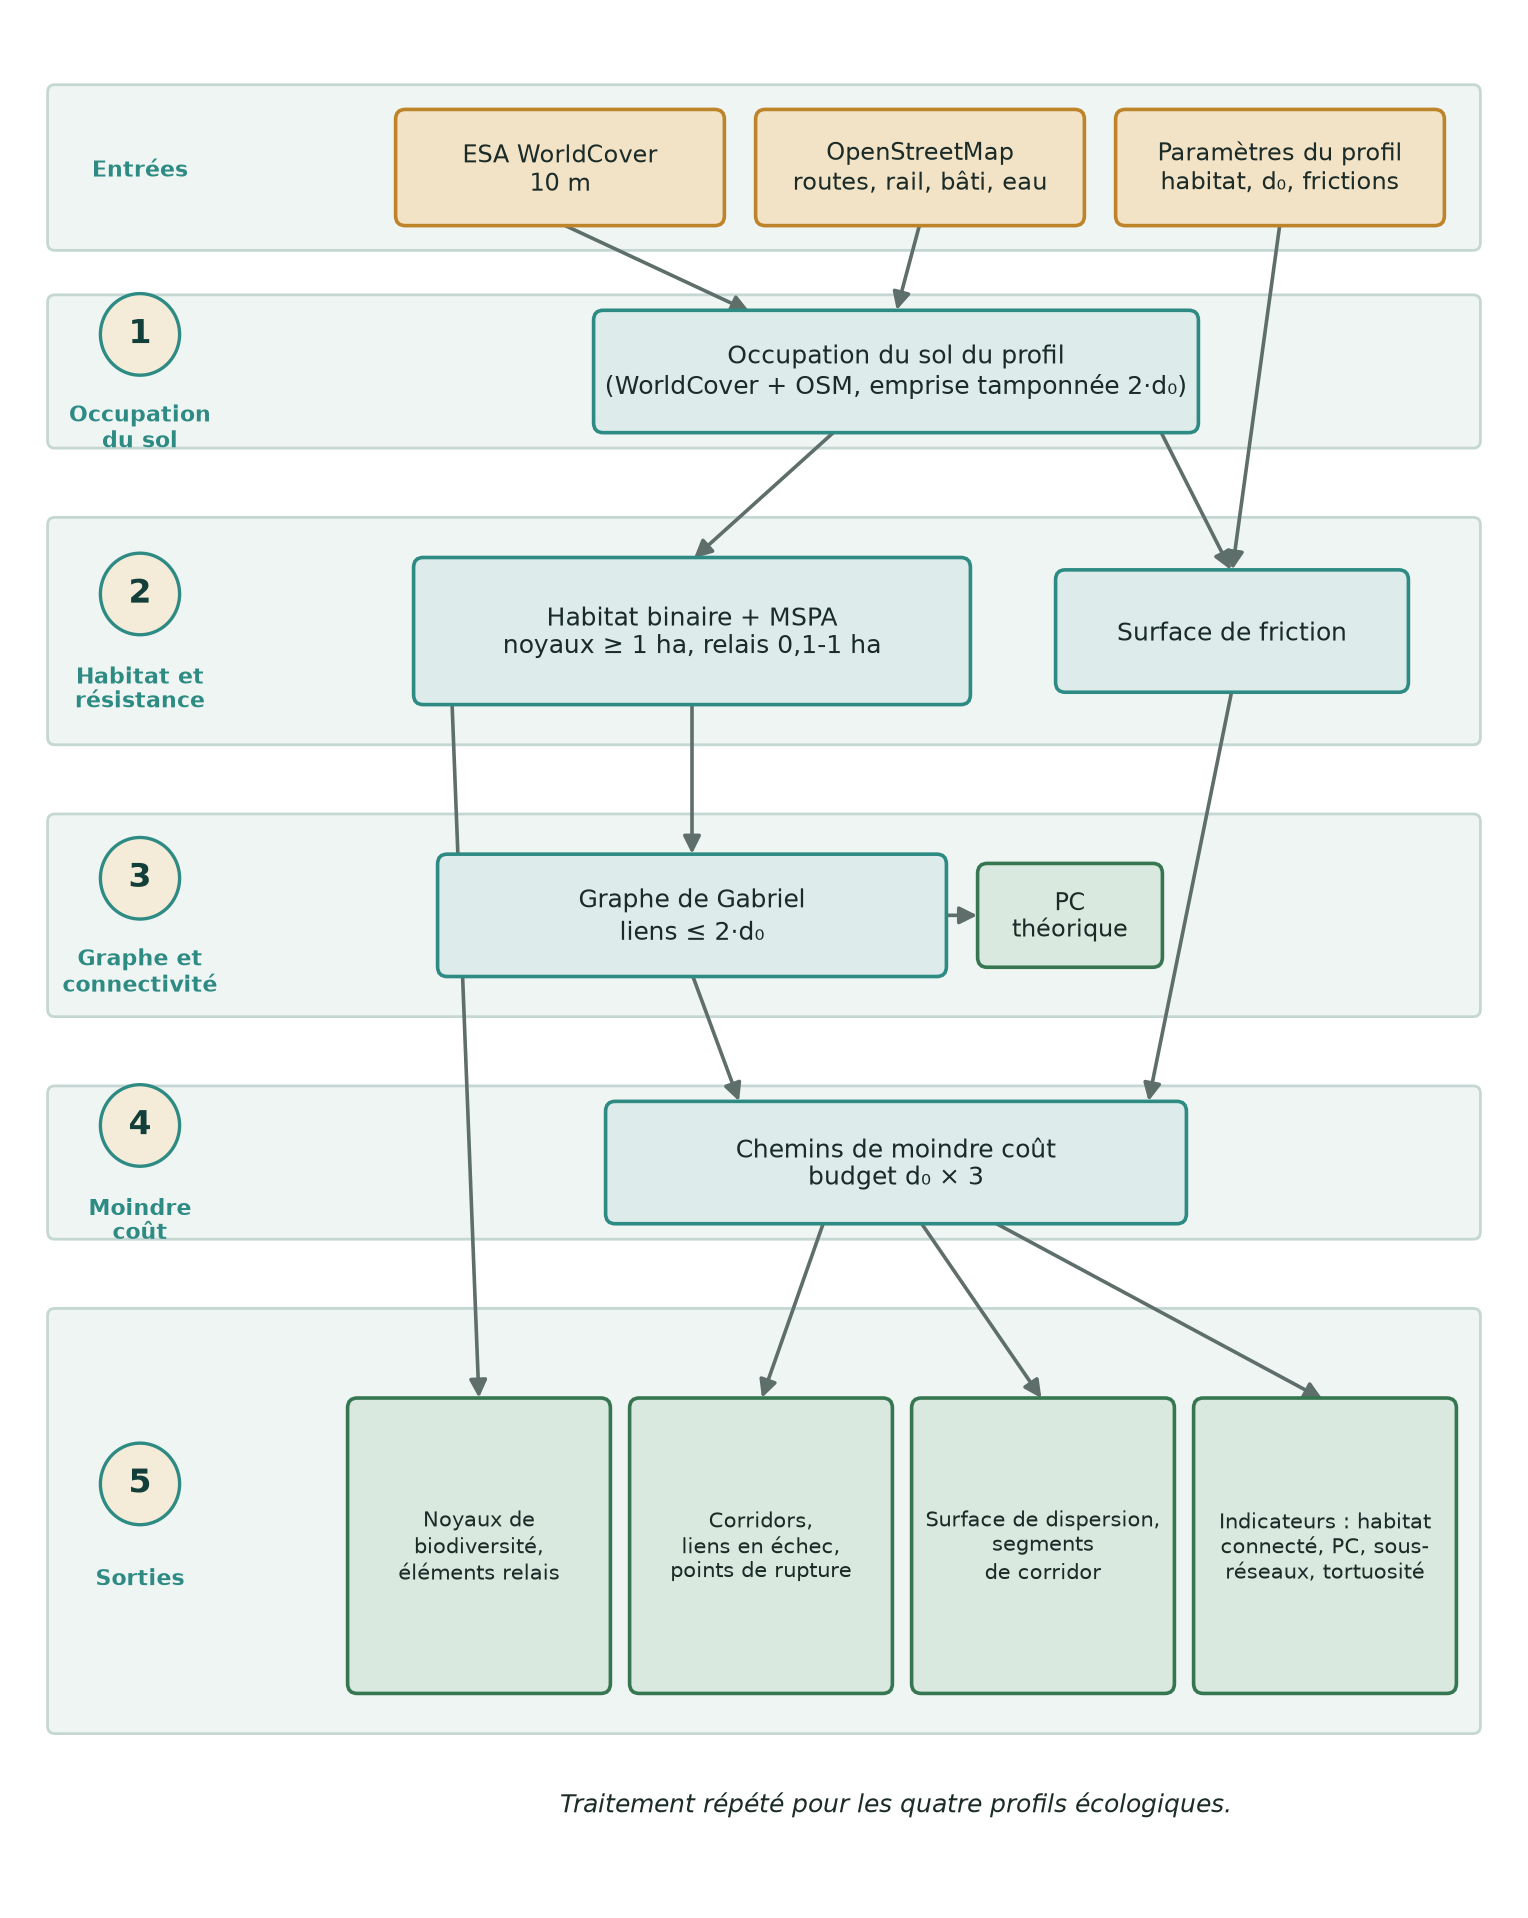
\includegraphics[width=0.98\textwidth]{figures/pipeline_chaine.png}
\caption{Schéma synoptique de la chaîne de traitement, des données d'entrée (WorldCover, OSM) aux sorties (noyaux, tracés de moindre coût, ruptures, dispersion, indicateurs).}
\label{fig:6}
\end{figure}

La première étape prépare la couche d'occupation du sol : le WorldCover est découpé sur l'emprise élargie par le tampon, puis les infrastructures OpenStreetMap y sont brûlées par-dessus (section 2.2). Une couche d'habitat binaire en est extraite, ne retenant que les classes d'habitat du profil écologique, puis soumise à une analyse morphologique de type MSPA \hyperref[sec:bibliographie]{(morphological spatial pattern analysis ; Vogt et al., 2007 ; Soille \& Vogt, 2009)}, implémentée sous scikit-image : une érosion suivie d'une dilatation isole les noyaux de biodiversité, taches dont le coeur compact dépasse un hectare, des espaces relais plus petits (de 0,1 à 1 hectare) qui jouent le rôle de pas japonais (\hyperref[fig:7]{Figure 7}).

Les seuils de surface retenus (noyau $\geq$ 1 ha, relais 0,1 à 1 ha) sont un choix de la chaîne, non une valeur imposée par la méthode : la segmentation morphologique classe les pixels selon la largeur de bord et ne fixe aucun seuil de surface canonique \hyperref[sec:bibliographie]{(Ostapowicz et al., 2008 ; Vogt \& Riitters, 2017)}. Le seuil de 1 ha est retenu comme surface minimale plausible d'un habitat fonctionnel en ville et pour la lisibilité de la restitution ; il rejoint directement la référence de calibration, le Cerema Dter Sud-Ouest \hyperref[sec:bibliographie]{(2025)} retenant, par la même méthode de c\oe{}urs compacts (érosion $-$10 m puis dilatation +10 m), un seuil de 1 ha pour les sous-trames arborée, arbustive et mixte (et 5 000 m² pour l'herbacée). Adopter un seuil unique de 1 ha est ici une simplification assumée.

\begin{figure}[H]
\centering
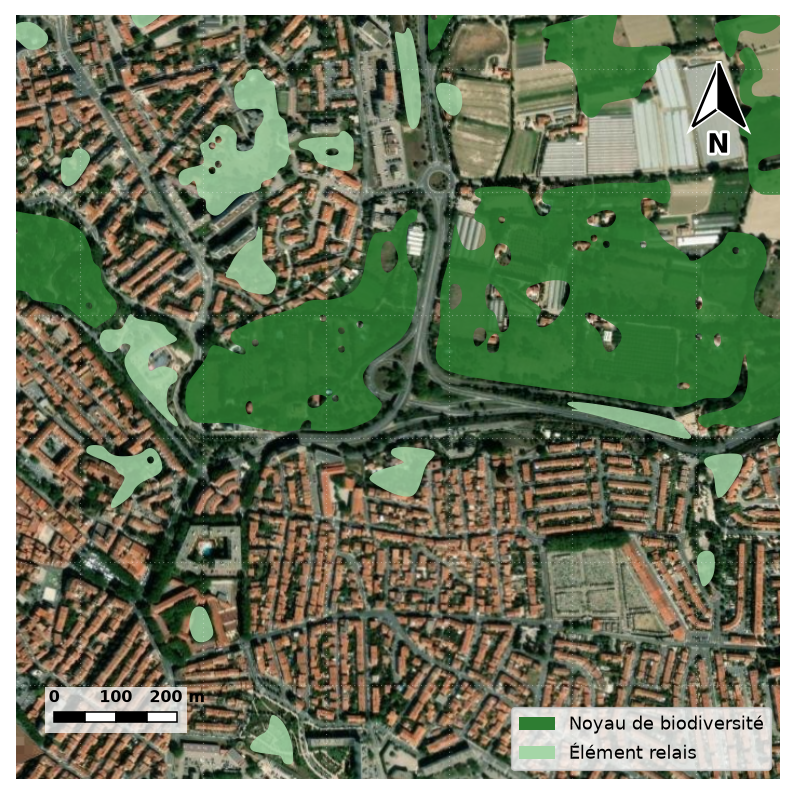
\includegraphics[width=0.98\textwidth]{figures/mspa_example.png}
\caption{Exemple de segmentation morphologique (MSPA) : noyaux de biodiversité (coeur $\geq$ 1 ha) et espaces relais (0,1 à 1 ha), profil du petit mammifère terrestre de lisière, sur un secteur de Perpignan.}
\label{fig:7}
\end{figure}

Ces taches deviennent les noeuds d'un graphe de Gabriel (networkx) construit sur les distances de bord à bord : deux taches sont reliées lorsque aucune autre tache ne s'intercale dans le cercle dont le segment les joignant constitue le diamètre (graphe de Gabriel ; Gabriel \& Sokal, 1969 ; \hyperref[fig:8]{Figure 8}), dans la limite d'une distance de recherche fixée à deux fois la distance de dispersion du profil écologique. À chaque lien est associée une probabilité de déplacement qui décroît avec la distance selon un noyau négatif-exponentiel, forme standard des graphes paysagers pour sa parcimonie \hyperref[sec:bibliographie]{(Foltête et al., 2012)} :

\begin{equation*}
p_{ij} = \exp(-d_{ij}/d_0)
\tag{1}
\end{equation*}

où d$_{i}$$_{j}$ est la distance de bord à bord entre les taches i et j, et d$_{0}$ la distance caractéristique de dispersion du profil écologique (\hyperref[sec:2.3]{§2.3}) : la distance à laquelle la probabilité de déplacement retombe à environ 37 \% (soit 1/e). Sur ce graphe est d'abord calculée la Probability of Connectivity \hyperref[sec:bibliographie]{(PC ; Saura \& Pascual-Hortal, 2007)}, qui mesure la connectivité potentielle à vol d'oiseau, indépendamment de la résistance du paysage :

\begin{equation*}
\mathrm{PC} = \frac{\sum_i \sum_j a_i\,a_j\,p_{ij}}{A^2}
\tag{2}
\end{equation*}

où a$_{i}$ et a$_{j}$ sont les surfaces des taches i et j, p$_{i}$$_{j}$ la probabilité de déplacement de l'équation (1) entre elles, et A la surface totale de la zone d'étude. La PC s'interprète comme la probabilité que deux points tirés au hasard dans la zone tombent dans des taches mutuellement accessibles ; elle est comprise entre 0 et 1.

Le choix du graphe de Gabriel parmi les graphes de proximité conditionne les connexions retenues. Trois variantes ont été implémentées et comparées avant de trancher. Les plus parcimonieuses (arbre couvrant minimal, graphe de voisinage relatif) ne conservent qu'un unique chemin entre taches et effacent la redondance des passages, tandis que les k plus proches voisins reposent sur un paramètre arbitraire qui tend à sur-connecter le réseau. Dans la hiérarchie d'inclusion de ces graphes de proximité \hyperref[sec:bibliographie]{(Toussaint, 1980)}, le graphe de Gabriel offre un compromis : il conserve des chemins alternatifs, plus réalistes écologiquement (un animal dispose rarement d'un itinéraire unique), sans relier deux taches qu'une troisième sépare, et fait ainsi ressortir plusieurs options de passage utiles à l'aide à la décision. Le niveau d'élagage du graphe influençant le résultat de connectivité \hyperref[sec:bibliographie]{(Minor \& Urban, 2008 ; Galpern et al., 2011)}, ce choix constitue un paramètre méthodologique assumé.

\begin{figure}[H]
\centering
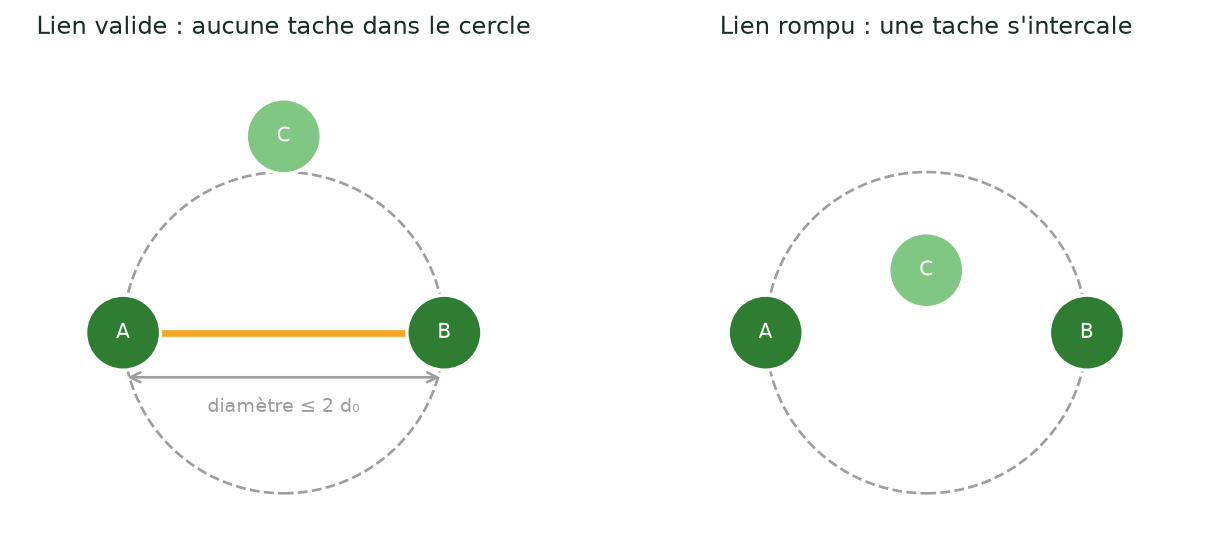
\includegraphics[width=0.98\textwidth]{figures/gabriel_criterion.png}
\caption{Construction du graphe de Gabriel : taches reliées selon le critère du cercle diamétral.}
\label{fig:8}
\end{figure}

La résistance du paysage est ensuite introduite : jusque-là les liens ne dépendaient que de la distance à vol d'oiseau, alors que le déplacement réel dépend aussi de la nature des milieux traversés, plus ou moins coûteux à franchir. Une surface de friction est dérivée de l'occupation du sol selon les coefficients de friction du profil écologique (détaillés en \hyperref[annexe:A]{annexe A}), puis chaque lien du graphe est tracé comme un chemin de moindre coût \hyperref[sec:bibliographie]{(Adriaensen et al., 2003)} sur cette surface (algorithme MCP géométrique de scikit-image). Un tel tracé est un trait de largeur nulle : le chemin optimal en coût n'indique pas l'emprise d'un corridor à aménager mais l'endroit où un lien est le plus probable \hyperref[sec:bibliographie]{(Pinto \& Keitt, 2009 ; Shirabe, 2018)}, ce qui justifie de parler de « lien » ou de « tracé de moindre coût » plutôt que de « corridor » pour ces sorties. Le coût accumulé d'un lien, exprimé en friction par mètre parcouru, est comparé à un budget de déplacement, égal à la distance de dispersion du profil multipliée par un coefficient favorable moyen de 3 :

\begin{equation*}
\mathrm{budget} = 3 \times d_0
\tag{3}
\end{equation*}

Ce facteur 3, convention de conversion d'une distance en coût reprise du Cerema, fixe le seuil de fonctionnalité : en deçà, le lien est jugé fonctionnel ; au-delà, ou s'il rencontre un obstacle infranchissable (bâti, grande rivière), il est marqué en échec. Les liens fonctionnels, les liens en échec et les points de rupture constituent les sorties cartographiques. Un point de rupture est l'intersection d'un lien bloqué avec une infrastructure ; il localise un lieu de conflit où un aménagement, par exemple un passage à faune, serait pertinent. Une carte de dispersion, surface de coût cumulé propagé depuis l'ensemble des taches sources \hyperref[sec:bibliographie]{(Adriaensen et al., 2003)} et bornée au budget de déplacement, complète ce dispositif : elle représente l'étendue qu'un profil peut atteindre depuis son habitat dans les limites de sa capacité de déplacement.

Le pré-filtre géométrique du graphe et le seuil de coût se cumulent. Le graphe de Gabriel ne relie deux taches que si leur distance euclidienne est inférieure à deux fois la distance de dispersion, et le coût du lien retenu est ensuite comparé au budget d$_{0}$ $\times$ 3, le critère de coût étant déterminant. Ce plafond de distance est volontairement large : un corridor réellement fonctionnel reste bien plus court que cette limite, de sorte que le pré-filtre géométrique n'écarte en pratique aucun corridor que le seul critère de coût aurait retenu.

Plusieurs indicateurs caractérisent enfin l'état du réseau. La Probability of Connectivity réelle est recalculée sur le réseau effectivement franchissable, en substituant à la distance à vol d'oiseau de l'équation (2) le coût de déplacement sur la surface de résistance. La surface équivalente connectée \hyperref[sec:bibliographie]{(Equivalent Connected Area ; Saura et al., 2011)} la traduit en unité de surface :

\begin{equation*}
\mathrm{EC} = \sqrt{\mathrm{PC}} \times A
\tag{4}
\end{equation*}

où A est la surface de la zone d'étude. L'EC s'interprète comme la taille d'un unique bloc d'habitat parfaitement connecté qui aurait la même PC que le réseau réel. Exprimée en hectares, elle et la part d'habitat connectée qui en découle (EC rapportée à la surface d'habitat) sont plus explicites pour un aménageur qu'une perte relative. Deux indicateurs complètent la lecture. Le nombre de sous-réseaux correspond au nombre de composantes connexes du réseau réel, sur les seules taches de la zone d'étude : un réseau connexe forme un seul ensemble relié (un seul sous-réseau), tandis que plusieurs sous-réseaux traduisent un réseau fragmenté en parties non reliées entre elles. La tortuosité des corridors rapporte leur longueur réelle à la distance à vol d'oiseau : proche de 1, le corridor est quasi rectiligne et peu contraint ; élevée, il contourne des obstacles par de longs détours, signe d'une matrice résistante et d'une connexion coûteuse. Les corridors sont aussi découpés en segments de tracé, c'est-à-dire les portions situées hors des taches d'habitat, qui localisent les espaces sur lesquels une action est possible.

\section{Implémentation et reproductibilité}\label{sec:2.5}

L'ensemble de la chaîne est implémenté en Python, sans recours à un logiciel de SIG externe ni à un outil de connectivité existant (Graphab, Conefor, Circuitscape, extension Biodispersal sous QGIS). Ce choix de ré-implémentation ne vise pas la nouveauté : les indices mobilisés sont ceux de la littérature (\hyperref[sec:1.5]{§1.5}), et la contribution réside dans leur assemblage en une chaîne unique. Passer par ces logiciels, conçus pour un usage interactif au cas par cas, aurait interdit l'automatisation de bout en bout, la reproductibilité sur des contextes contrastés et l'actualisation dans le temps visées ici (objectif 3) ; les ré-implémenter donne le contrôle et la transparence du calcul, au prix d'un effort de développement et de la charge de vérifier que chaque étape reproduit la méthode de référence (\hyperref[sec:4.4]{§4.4}). Les traitements raster reposent sur xarray et rioxarray, les traitements vectoriels sur geopandas et shapely, la rastérisation sur rasterio, le graphe sur networkx, et les calculs de moindre coût comme de morphologie sur scikit-image (versions précises en \hyperref[annexe:A]{annexe A}.4) ; le calcul de la Probability of Connectivity est optimisé : plutôt que de parcourir une à une toutes les paires de taches, il s'appuie sur un unique parcours de plus court chemin et un produit matriciel, beaucoup plus rapides. Le produit d'occupation du sol WorldCover est récupéré via Google Earth Engine (xee).

L'architecture sépare la configuration du code. Les paramètres de chaque profil écologique (habitat, distance de dispersion, frictions) sont isolés dans un fichier de configuration dédié, et les chemins de sortie sont centralisés. Un script unique pilote l'exécution, par territoire et, au besoin, par profil écologique, et produit pour chaque couple une arborescence de sorties normalisée (\hyperref[fig:9]{Figure 9}) : rasters d'occupation du sol, d'habitat, de friction et de dispersion ; couches vectorielles des noeuds, tracés de moindre coût, liens en échec et segments de tracé ; tableau d'indicateurs. Cette organisation rend la chaîne automatisable et reproductible, une même commande régénérant l'intégralité des résultats d'un territoire. Le code est versionné dans un dépôt Git \hl{[À COMPLÉTER : lien du dépôt]}, organisé autour du fichier de configuration, du script d'exécution et des modules de traitement (préparation des données, connectivité, restitution).

\begin{figure}[H]
\centering
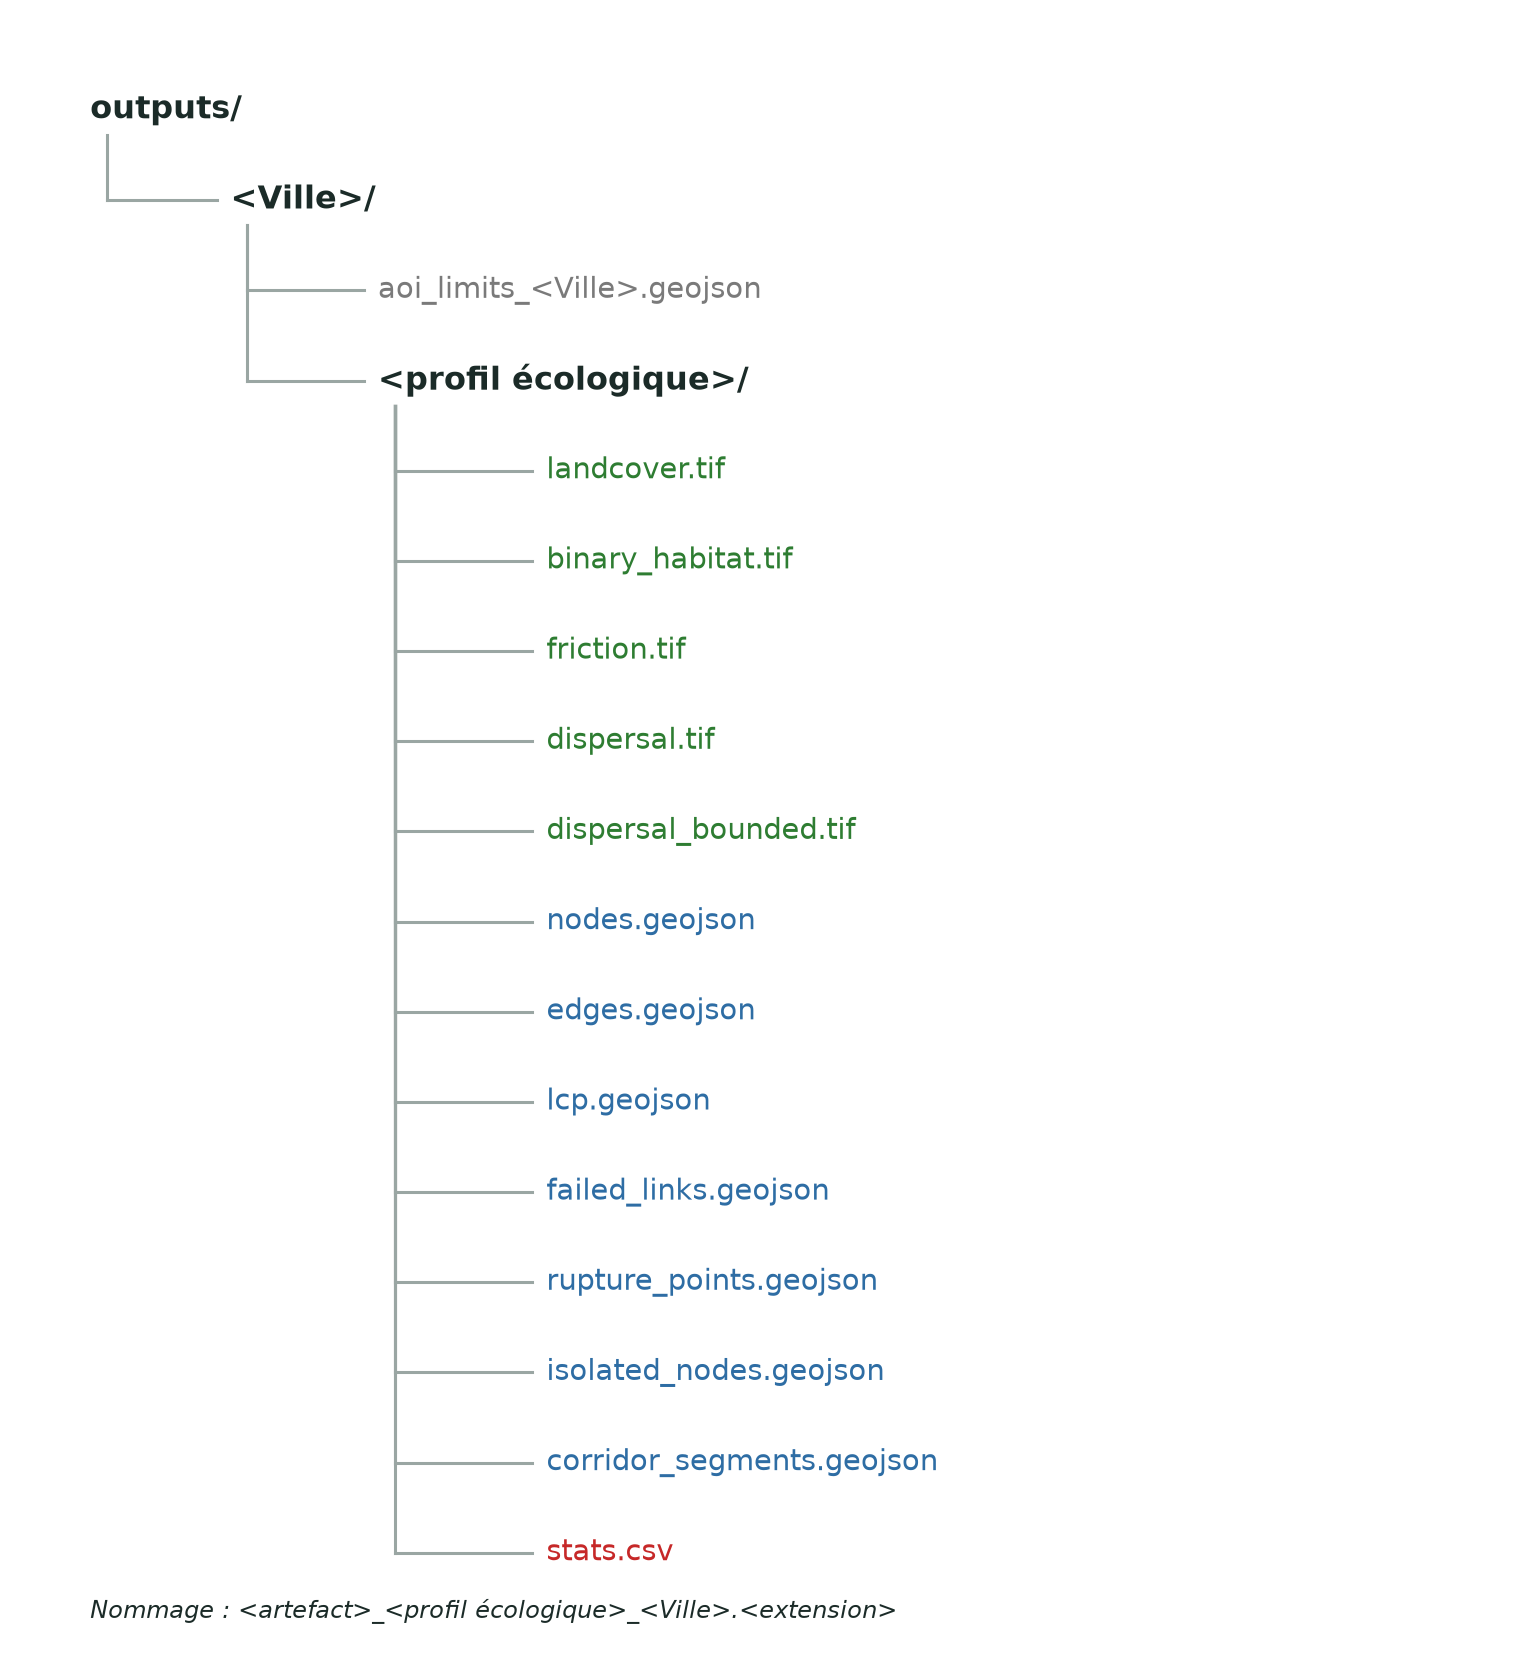
\includegraphics[width=0.98\textwidth]{figures/arborescence_sorties.png}
\caption{Arborescence normalisée des sorties, par territoire et par profil écologique.}
\label{fig:9}
\end{figure}

La chaîne intègre enfin un contrôle automatisé de ses sorties (`output\_check.py`), exécuté à la fin de chaque production : conformité de la projection (métrique, UTM), présence et non-vacuité des couches attendues (noyaux, corridors), présence des indicateurs de tête, et plausibilité physique des valeurs (frictions comprises entre 1 et 100 avec obstacles en coût infini, coûts de dispersion bornés au budget de déplacement 3 $\times$ d$_{0}$). Il signale toute anomalie avant exploitation ; les vingt-quatre jeux des six territoires l'ont passé sans anomalie. La robustesse des sorties aux choix de calibration et leur confrontation à des sources externes relèvent en revanche de la discussion (\hyperref[chap:4]{chapitre 4}).

\section{Restitution : le tableau de bord}\label{sec:2.6}

Les sorties cartographiques ne deviennent un outil d'aide à la décision que si elles sont rendues lisibles pour des aménageurs non spécialistes. Cette restitution prend la forme d'un tableau de bord interactif, accessible en ligne, qui présente pour chaque territoire et chaque profil écologique les différentes couches produites (noyaux de biodiversité, tracés de moindre coût, points de rupture, surface de dispersion) que l'utilisateur peut afficher et superposer, ainsi que les indicateurs de connectivité associés. Le tableau de bord permet d'explorer visuellement le réseau écologique d'un territoire et de comparer des scénarios d'aménagement (\hyperref[fig:10]{Figure 10}). Les sorties du pipeline sont d'abord converties en couches légères : les géométries (aire d'étude, taches d'habitat, tracés de moindre coût, barrières, points de rupture) au format GeoJSON, les indicateurs au format CSV, et le raster de dispersion en GeoTIFF. Le tableau de bord est une application web développée en Python avec Plotly Dash, intégrée à l'environnement de tableaux de bord de Murmuration ; la cartographie s'appuie sur Leaflet. L'utilisateur affiche et superpose les couches, dessinées directement dans le navigateur ; le raster de dispersion, plus lourd, est servi sous forme de tuiles dans la version en ligne, tandis que la version locale le charge directement. L'accès est réservé aux utilisateurs authentifiés de Murmuration. À ce stade, le tableau de bord constitue une brique autonome, bâtie sur les gabarits de Murmuration, et son intégration à la plateforme UrbiVerde n'est pas encore réalisée.

\begin{figure}[H]
\centering
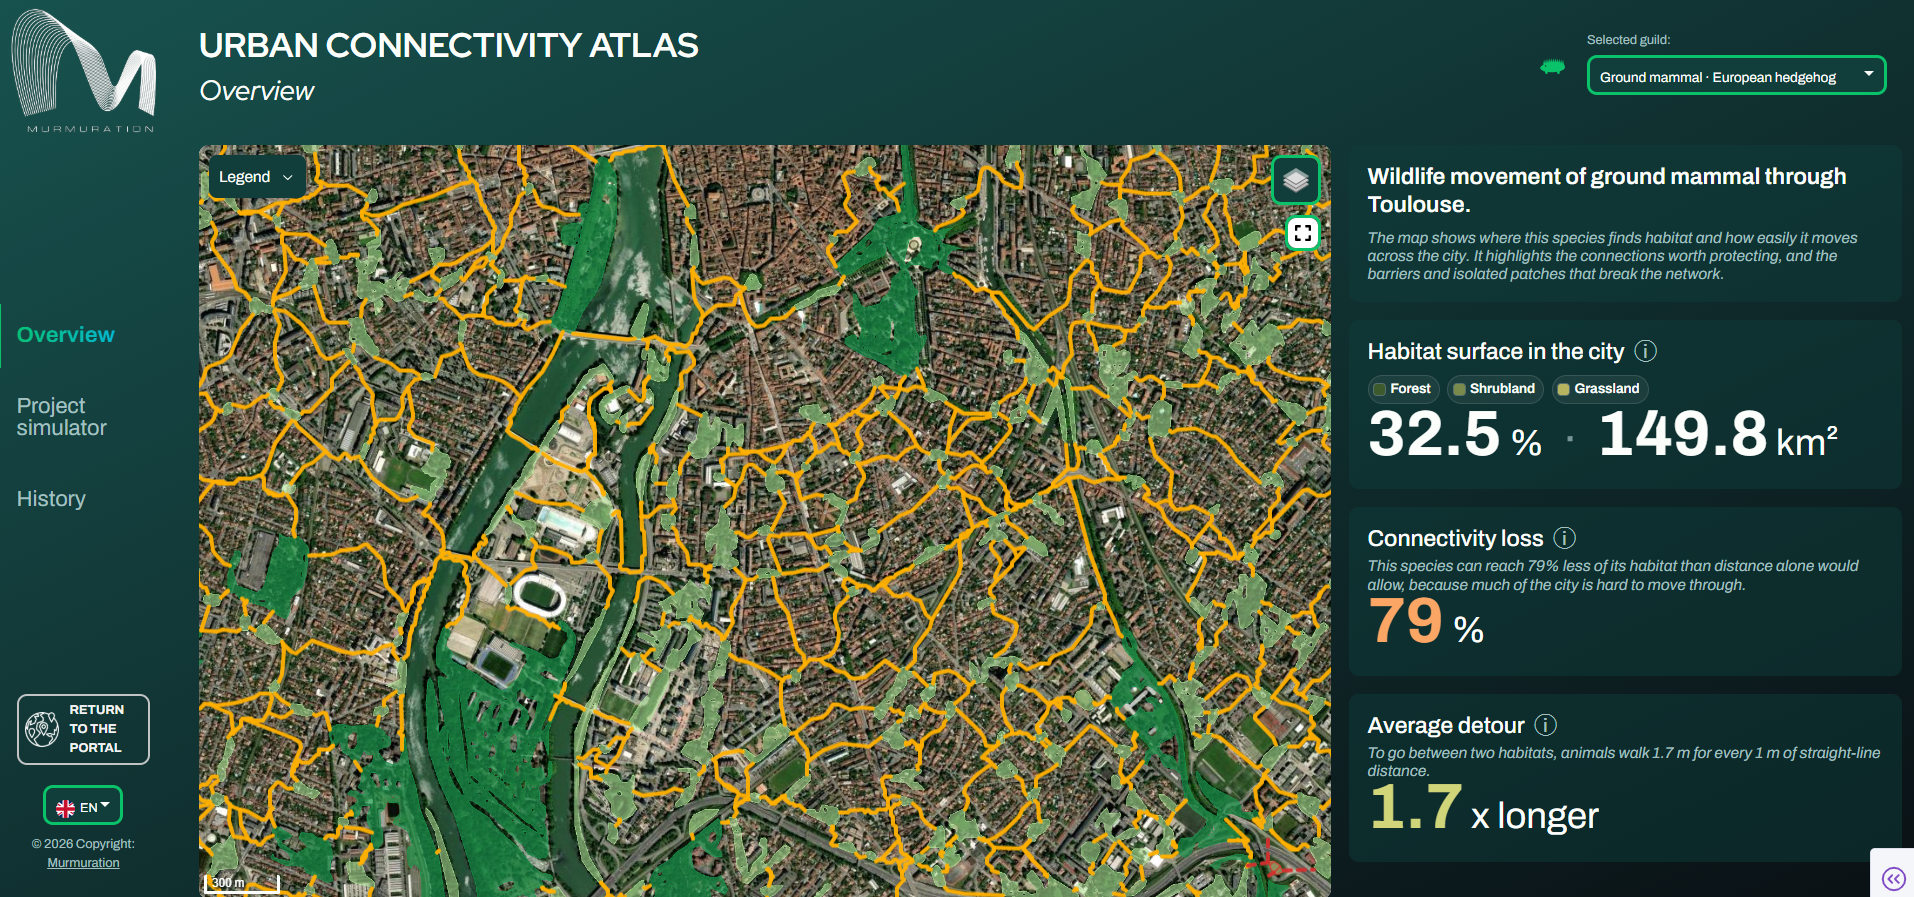
\includegraphics[width=0.98\textwidth]{figures/dashboard_capture.png}
\caption{Capture d'écran du tableau de bord interactif (sélection d'un territoire et d'un profil écologique, couches superposables, indicateurs).}
\label{fig:10}
\end{figure}

\chapter{Résultats}\label{chap:3}

Ce chapitre présente, de façon descriptive, les sorties de la chaîne sur les six territoires : les couches produites (3.1), les indicateurs de connectivité par profil écologique (3.2) et leur variation entre territoires (3.3), la réponse des sorties aux variations de calibration (3.4), leur confrontation à des observations et à une méthode de référence (3.5) et l'effet d'un scénario d'aménagement (3.6). L'interprétation de ces résultats est développée au \hyperref[chap:4]{chapitre 4}.

\section{Un jeu de sorties normalisé pour chaque couple territoire-profil}\label{sec:3.1}

Pour chaque couple (territoire, profil écologique), la chaîne produit le jeu de sorties normalisé décrit au \hyperref[chap:2]{chapitre 2} (\hyperref[fig:6]{Figures 6 et 9}) : rasters, couches vectorielles (noyaux de biodiversité, éléments relais, liens fonctionnels, liens en échec, points de rupture) et tableau d'indicateurs. Sur les six territoires et les quatre profils écologiques, vingt-quatre jeux de résultats ont été générés, tous exprimés dans la projection métrique locale (UTM) et directement mobilisables en SIG comme dans le tableau de bord (\hyperref[fig:11]{Figure 11}).

\begin{figure}[H]
\centering
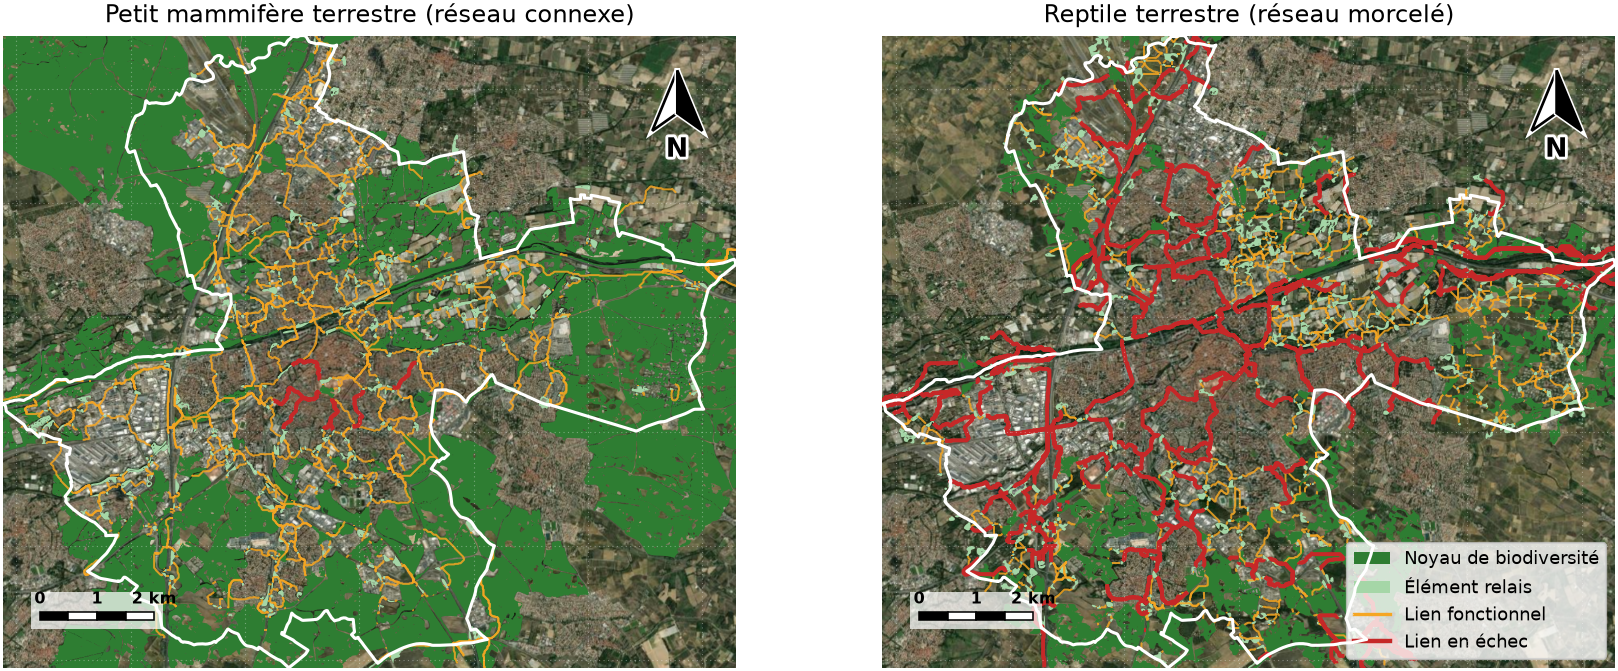
\includegraphics[width=0.98\textwidth]{figures/sorties_perpignan.png}
\caption{Sorties de la chaîne sur Perpignan pour deux profils écologiques contrastés : le petit mammifère terrestre (à gauche, réseau connexe) et le reptile terrestre (à droite, réseau morcelé). Noyaux de biodiversité, éléments relais, liens fonctionnels et liens en échec.}
\label{fig:11}
\end{figure}

À titre d'exemple, le profil écologique du petit mammifère terrestre sur Perpignan compte 525 noyaux de biodiversité et 1 421 espaces relais, reliés par 1 075 liens fonctionnels. Perpignan sert d'illustration parce qu'il offre, sur une emprise compacte, le contraste le plus lisible entre profils écologiques (\hyperref[sec:3.3]{§3.3}) : le réseau y passe d'un bloc unique et bien connecté pour le petit mammifère terrestre à un réseau très morcelé pour le reptile.

\section{Une part d'habitat connecté très variable selon le profil}\label{sec:3.2}

L'indicateur retenu au premier plan est la part d'habitat fonctionnellement connecté (définie au \hyperref[chap:2]{chapitre 2}) : normalisée entre 0 et 100 \%, elle reste comparable entre des territoires d'emprises différentes, là où la surface connectée équivalente croît avec l'étendue. Le nombre de sous-réseaux, ou composantes connexes (sous-ensembles de taches toutes accessibles les unes aux autres), la complète. Le Tableau 3 en donne la médiane et l'étendue sur les six territoires, par profil écologique ; la tortuosité et les dénombrements (noyaux, relais, corridors, ruptures) figurent dans les jeux de sorties et en \hyperref[annexe:D]{annexe D}.

\begin{table}[H]
\centering
\caption{Récapitulatif des indicateurs par profil écologique, sur les six territoires (étendue et médiane).}
\begin{tabularx}{\textwidth}{>{\raggedright\arraybackslash}X >{\raggedright\arraybackslash}X >{\raggedright\arraybackslash}X >{\raggedright\arraybackslash}X}
\toprule
\textbf{Profil écologique (espèce repère)} & \textbf{Sous-réseaux (méd. [min--max])} & \textbf{Habitat connecté (méd. [min--max])} & \textbf{Territoires à réseau connexe} \\
\midrule
Petit mammifère terrestre (hérisson) & 1 [1--2] & 67 \% [40--83] & 5 / 6 \\
Mammifère arboricole (écureuil) & 1 [1--11] & 28 \% [17--82] & 4 / 6 \\
Oiseau de lisière (fauvette) & 2 [1--28] & 24 \% [15--69] & 3 / 6 \\
Reptile terrestre (lézard) & 7 [3--14] & 23 \% [9--45] & 0 / 6 \\
\bottomrule
\end{tabularx}
\end{table}

Les valeurs se distribuent entre deux extrêmes. Le petit mammifère terrestre est partout le profil le mieux connecté : son réseau reste connexe dans cinq territoires sur six et sa part d'habitat connecté est la plus élevée (médiane 67 \%). Le reptile terrestre est à l'opposé : son réseau n'est jamais connexe (3 à 14 sous-réseaux) et sa part d'habitat connecté est la plus basse (médiane 23 \%). Le mammifère arboricole et l'oiseau de lisière sont intermédiaires, avec une forte variabilité entre territoires (l'oiseau de lisière reste connexe à Nancy, à La Roche-sur-Yon et à Kourou, mais se fragmente en vingt-huit sous-réseaux à La Rochelle). L'écart entre profils peut être marqué sur un même territoire : à Perpignan, le reptile terrestre connecte 23 \% de son habitat en quatorze sous-réseaux, quand le petit mammifère terrestre en connecte 64 \% en un seul réseau connexe ; les points de rupture des profils terrestres s'y concentrent sur les axes routiers.

Les surfaces de dispersion rendent ce contraste visible (\hyperref[fig:12]{Figure 12}) : celle du petit mammifère terrestre couvre le territoire d'un vert quasi continu, tandis que celle du reptile vire à l'orange et au rouge au contact du tissu urbain.

\begin{figure}[H]
\centering
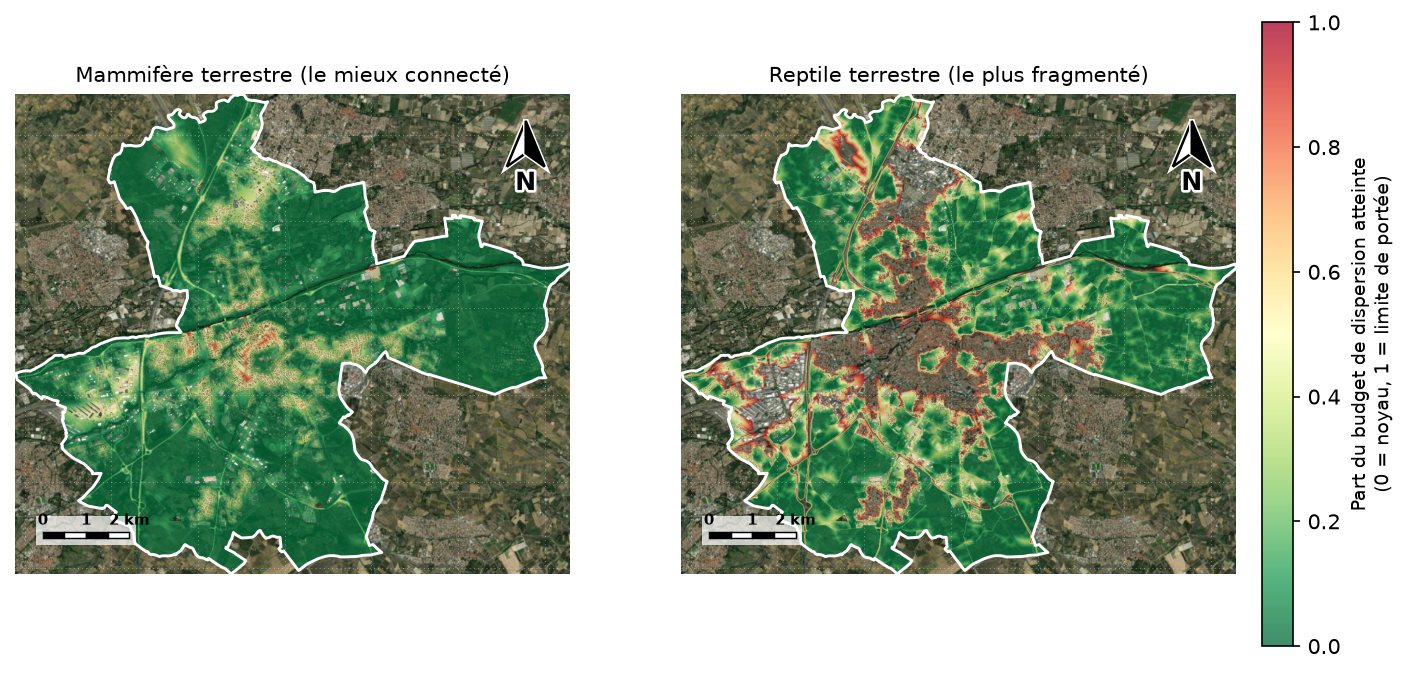
\includegraphics[width=0.98\textwidth]{figures/dispersion_comparee.png}
\caption{Surfaces de dispersion comparées de deux profils écologiques contrastés sur un même territoire. Le petit mammifère terrestre couvre la quasi-totalité de la zone en restant loin de son budget de dispersion (vert) ; le reptile atteint vite sa limite de portée (orange à rouge), surtout au contact du tissu urbain.}
\label{fig:12}
\end{figure}

\section{Contrastes entre territoires : un test de transposabilité}\label{sec:3.3}

Appliquée à l'identique aux six territoires, sans aucun réglage propre à chaque site, la chaîne produit sur chacun un jeu de sorties complet, des façades atlantique et continentale au climat méditerranéen et équatorial. C'est le résultat direct de l'objectif de transposabilité (objectif 5) : une même commande tourne de bout en bout sur des contextes bioclimatiques très différents. Les niveaux de connectivité obtenus varient fortement d'un territoire à l'autre. Pour le petit mammifère terrestre, la part d'habitat connecté s'échelonne de 83 \% à La Roche-sur-Yon à 40 \% à La Rochelle, en passant par Nancy (71 \%), Perpignan (64 \%) et Toulouse (52 \%) ; Kourou se distingue par des parts élevées sur tous les profils écologiques (45 à 82 \%). Le détail par territoire et par profil figure en \hyperref[annexe:D]{annexe D}.

Cette variation touche tous les profils, avec une amplitude croissante des plus mobiles aux moins mobiles : le mammifère arboricole et l'oiseau de lisière passent d'un réseau connexe (Nancy, Kourou) à une forte fragmentation à La Rochelle (onze et vingt-huit sous-réseaux), tandis que le reptile n'est connexe sur aucun territoire, son nombre de sous-réseaux s'étageant de trois à quatorze. Surtout, le classement des territoires n'est pas le même selon le profil : un territoire favorable au petit mammifère terrestre ne l'est pas nécessairement pour les profils boisés ou thermophiles (\hyperref[fig:19]{Figure 19}). Ces écarts sont ici décrits ; leur interprétation au regard de la forme urbaine relève de la discussion (\hyperref[sec:4.2]{§4.2}).

\section{Sensibilité des indicateurs au paramétrage de la calibration}\label{sec:3.4}

Les coefficients de friction et les distances de dispersion sont fixés à partir de la littérature et de la méthode du Cerema Dter Sud-Ouest \hyperref[sec:bibliographie]{(2025)} plutôt que mesurés sur le terrain : ce sont les entrées les moins contraintes de la chaîne, où se concentre l'essentiel de son incertitude (\hyperref[sec:1.5.1]{§1.5.1}). Avant d'accorder une portée à un résultat, il faut donc savoir s'il tient à un choix de paramétrage ou s'il résiste à une variation plausible de ces valeurs. C'est l'objet de l'analyse de sensibilité : délimiter jusqu'où ses conclusions restent stables, non confirmer que le modèle dit vrai.

Deux paramètres sont balayés sur une plage large : la distance de dispersion d$_{0}$, de 50 à 120 \% de sa valeur de référence, qui commande la portée ; et le contraste de friction, c'est-à-dire l'écart de coût de déplacement entre l'habitat et la matrice, de 0 (matrice homogène, aucun écart) à 200 \% (écart doublé), qui module la résistance différenciée de la matrice. Plutôt que de fixer a priori une amplitude de perturbation, on trace la courbe de réponse de chaque territoire et l'on y lit deux choses : la sensibilité au voisinage des valeurs de référence, et la marge, c'est-à-dire la distance entre le paramétrage de référence et un changement de régime (gain ou perte de connexité). Deux indicateurs sont suivis, la part d'habitat connecté (continue) et le nombre de sous-réseaux (compte gradué de la fragmentation). La synthèse par territoire et par profil écologique figure en \hyperref[annexe:E]{annexe E}.

Le contraste de friction ressort comme le levier dominant. À contraste nul, la matrice n'oppose plus de résistance différenciée et la part connectée bondit vers un réseau quasi connexe pour tous les profils (à Perpignan, de 64 à 96 \% pour le petit mammifère terrestre, de 23 à 50 \% pour le reptile), puis décroît à mesure que le contraste se renforce. Cette amplitude, du même ordre ou supérieure à celle de d$_{0}$, désigne l'écart de résistance entre classes d'occupation du sol, plus que le niveau absolu des coûts, comme le paramètre déterminant \hyperref[sec:bibliographie]{(Bowman et al., 2020)}.

La distance de dispersion agit de façon plus graduée et monotone, et sa marge dépend du profil écologique et du territoire. Le petit mammifère terrestre est robuste : son réseau ne se scinde qu'aux plus faibles portées, en deçà d'environ 60 à 70 \% de d$_{0}$ selon le territoire (il reste connexe sur toute la plage testée à Nancy), de sorte qu'il faudrait une erreur importante sur sa portée pour changer le diagnostic. Le reptile est à l'opposé : jamais connexe sur toute la plage, déjà au-delà du seuil au paramétrage de référence, il ne se distingue que par son degré de fragmentation, qui s'étage fortement (à Perpignan, de vingt-cinq sous-réseaux à d$_{0}$ réduit de moitié à quatorze au paramétrage de référence ; à La Rochelle, jusqu'à près de cent aux plus faibles portées). Le mammifère arboricole et l'oiseau de lisière sont intermédiaires, connexes au voisinage des valeurs de référence et fragmentés aux faibles portées.

Kourou fait exception sur l'axe de la dispersion : la part connectée du petit mammifère terrestre y reste plate (69 à 70 \% de 50 à 120 \% de d$_{0}$), sa matrice forestière équatoriale étant si perméable que la portée n'y change presque rien ; le contraste, lui, y agit comme ailleurs (97 \% à contraste nul). La sensibilité dépend donc du territoire : le même écart de paramètre est inerte à Kourou et sensible dans les tissus fragmentés, ce qui est en soi un résultat (\hyperref[fig:13]{Figures 13 et 14}).

Au total, l'analyse conforte l'usage comparatif de l'outil : l'ordre entre profils écologiques et entre territoires, et le fait qu'un réseau soit ou non connexe, se maintiennent sur la plage testée, tandis que les valeurs absolues se déplacent. Elle borne aussi ce qui peut en être conclu, comme le précisent les deux réserves suivantes.

Deux réserves encadrent cette lecture. La perturbation ne fait varier qu'un paramètre à la fois : une bascule par combinaison de la dispersion et du contraste n'est pas capturée, la marge étant mesurée le long d'un seul axe. Et l'analyse teste la robustesse au choix des paramètres, non l'accord des sorties avec le terrain, qui relève de la validation (\hyperref[sec:4.4]{§4.4}).

\begin{figure}[H]
\centering
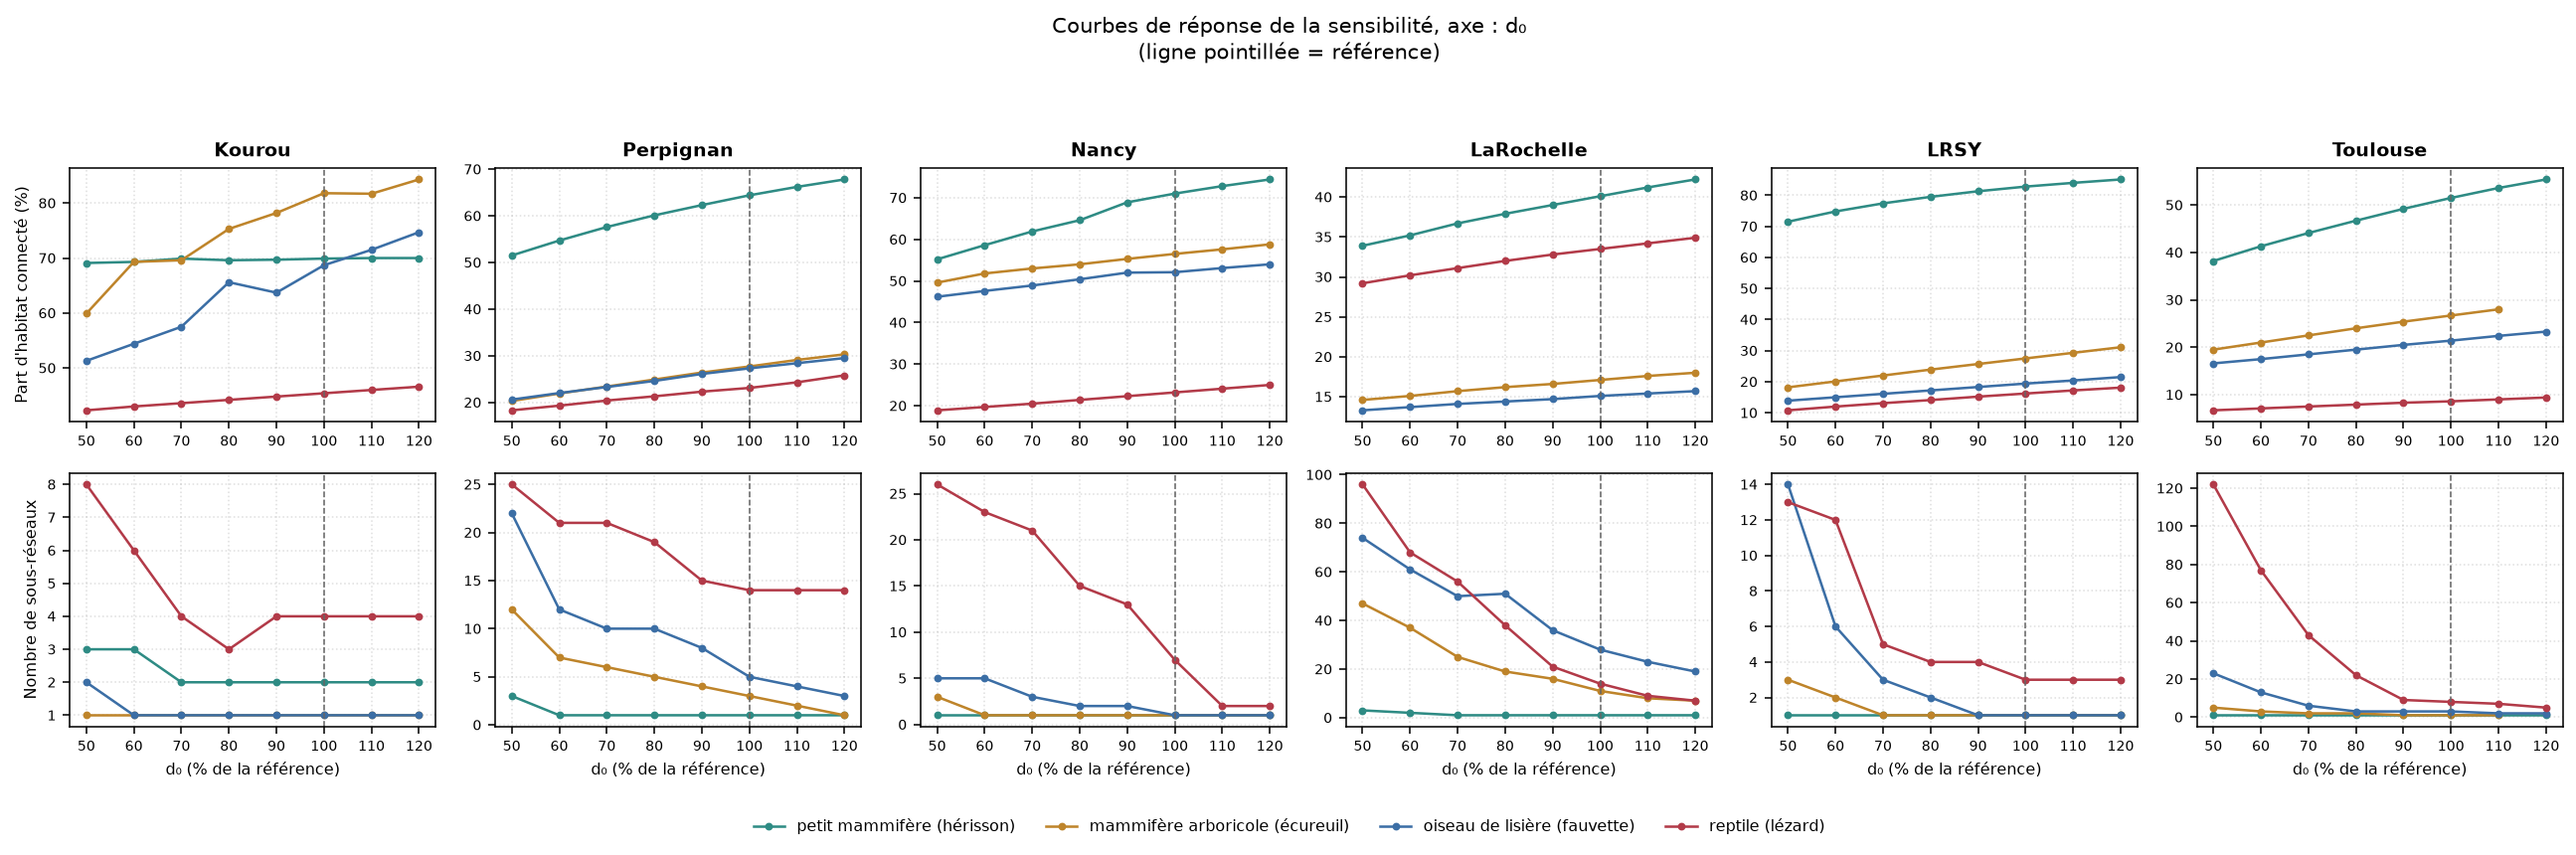
\includegraphics[width=0.98\textwidth]{figures/sens_curves_d0.png}
\caption{Courbes de réponse à la distance de dispersion (50 à 120 \% de la référence). Part d'habitat connecté (en haut) et nombre de sous-réseaux (en bas), un panneau par territoire (colonnes), une couleur par profil écologique ; ligne pointillée = référence.}
\label{fig:13}
\end{figure}

\begin{figure}[H]
\centering
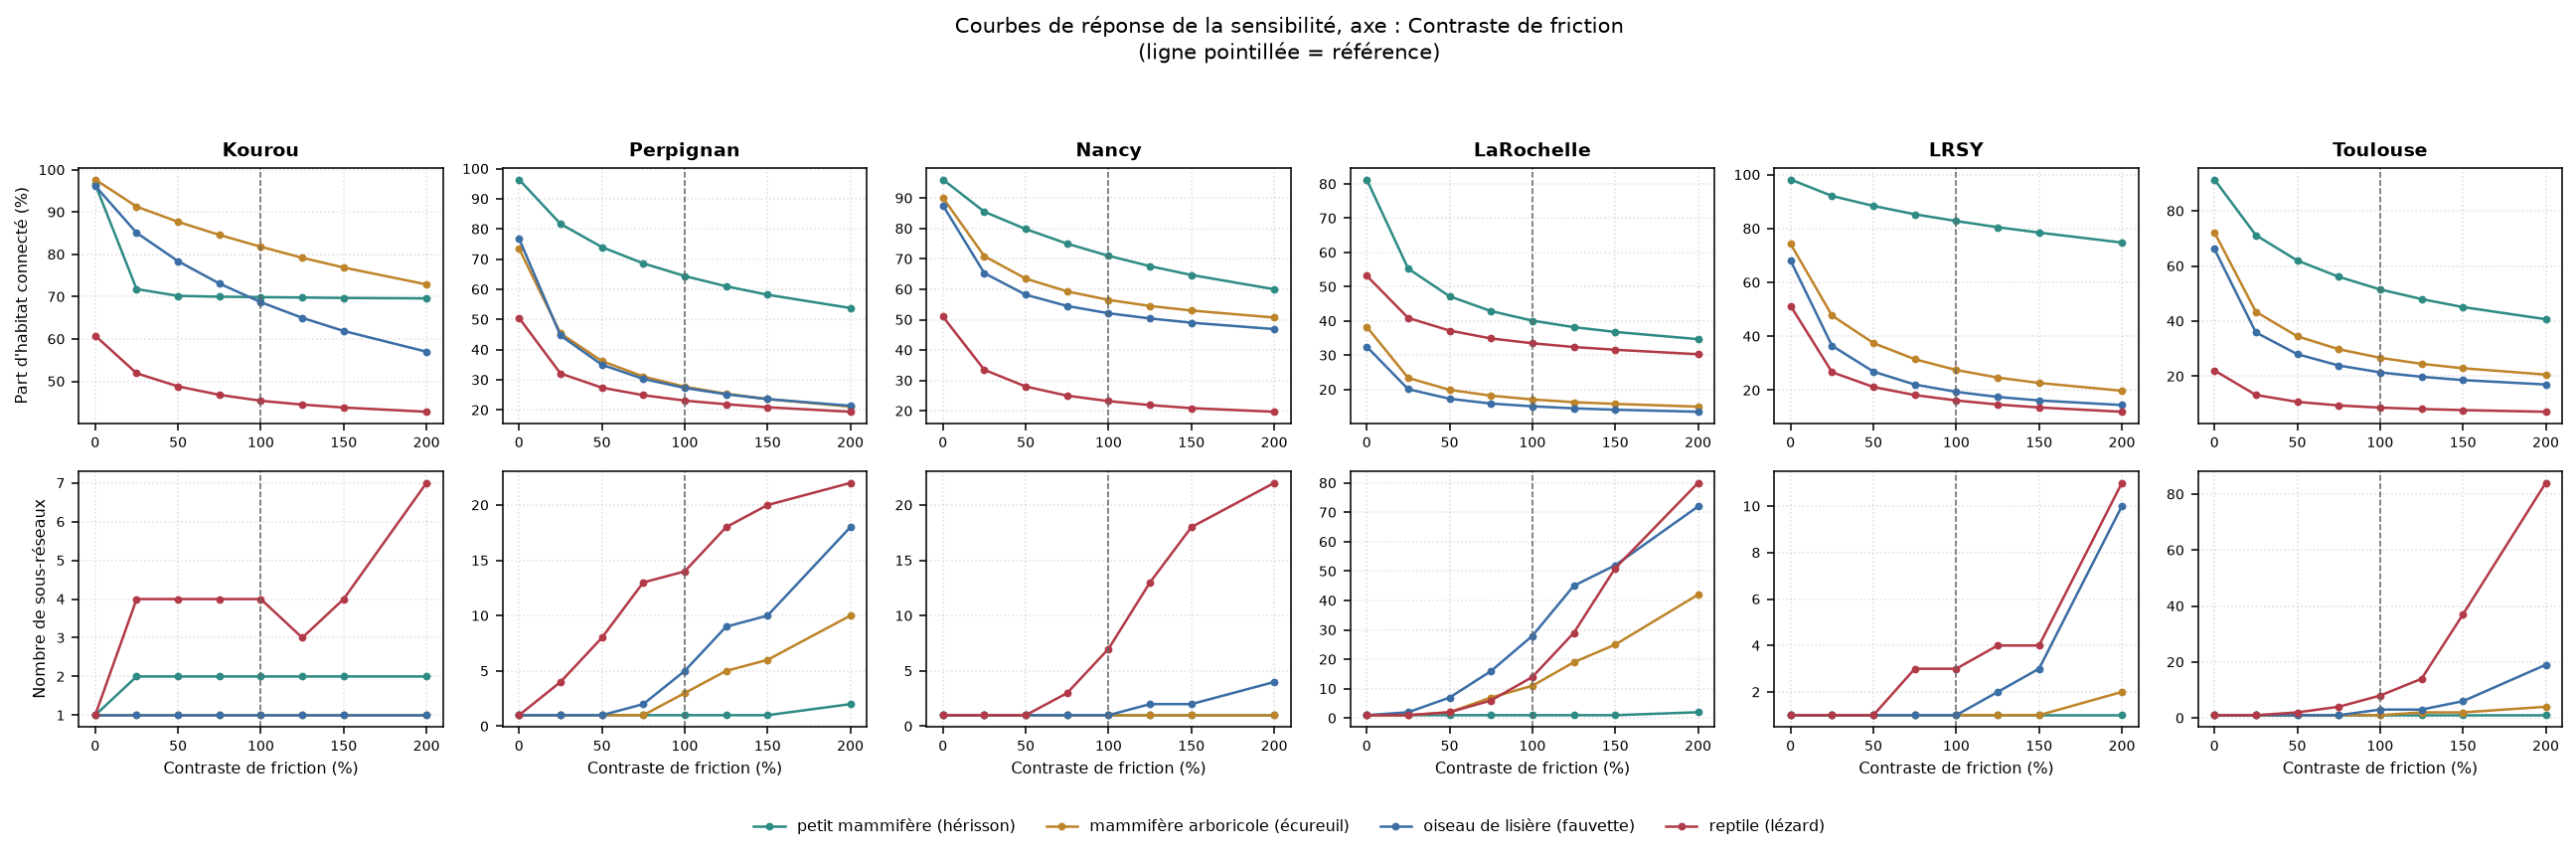
\includegraphics[width=0.98\textwidth]{figures/sens_curves_contrast.png}
\caption{Courbes de réponse au contraste de friction (0 à 200 \%).}
\label{fig:14}
\end{figure}

\section{Confrontation aux observations GBIF et à la méthode du Cerema}\label{sec:3.5}

Deux confrontations externes ont été menées, dont la portée est discutée en section 4.4.

La première, aux occurrences GBIF, teste le côté habitat du modèle, c'est-à-dire si les espèces d'un profil se trouvent là où le modèle place leur habitat, et non le flux le long des corridors. Les couches modélisées ont été confrontées aux occurrences GBIF d'un groupe de quatre espèces par profil écologique (liste en \hyperref[annexe:B]{annexe B}), sur les cinq territoires métropolitains. Les occurrences GBIF reflétant autant la répartition des observateurs que celle des espèces (biais d'échantillonnage, \hyperref[sec:1.5.3]{§1.5.3}), deux précautions précèdent l'analyse. Les relevés sont d'abord filtrés : seules sont retenues les observations de terrain dont l'incertitude de localisation annoncée est inférieure à 100 m et postérieures à 2016. Ce seuil de 100 m est courant pour le nettoyage des occurrences \hyperref[sec:bibliographie]{(Zizka et al., 2019)} ; il correspond aussi à la taille d'une maille de noyau (1 ha, soit 100 m de côté), c'est-à-dire à la finesse avec laquelle chaque occurrence peut être rattachée à une couche du modèle sans ambiguïté. La borne de 2016 conserve les relevés contemporains du millésime d'occupation du sol utilisé et limite les décalages liés aux changements d'usage. Les relevés sont ensuite sous-échantillonnés à une occurrence par cellule, ce qui efface les grappes d'observations répétées au même endroit. Chaque occurrence est ensuite affectée à la couche modélisée qui la contient (noyau, relais, corridor ou matrice). Pour isoler la sélection réelle de l'effort d'observation, biais spatial, temporel et taxonomique bien documenté des données d'occurrence \hyperref[sec:bibliographie]{(Boakes et al., 2010 ; El-Gabbas, 2026 ; Melis et al., 2025)}, un ratio de sélection \hyperref[sec:bibliographie]{(usage rapporté à la disponibilité ; Johnson, 1980 ; Manly et al., 2002)} compare la part des occurrences de l'espèce dans une classe à celle d'un fond d'observation constitué de toutes les espèces de sa classe taxonomique (mammifères, oiseaux ou reptiles) relevées sur le même territoire. Ce fond subit exactement le même biais d'observation que l'espèce cible, si bien que le ratio se lit directement : proche de un, la classe est fréquentée comme le prédit le seul effort d'observation ; nettement supérieur à un, elle est sélectionnée ; inférieur à un, elle est évitée. Un intervalle de confiance à 95 \% par bootstrap accompagne chaque ratio et tranche lorsqu'il exclut un. Sur les ratios agrégés (\hyperref[fig:15]{Figure 15}), les espèces d'habitat boisé sont sur-représentées dans les noyaux : l'oiseau de lisière y affiche un ratio de 1,80 (intervalle 1,65 à 1,95) et un ratio de 0,69 dans la matrice, le mammifère arboricole un ratio de 1,68 dans les noyaux et de 0,50 dans la matrice. Le petit mammifère terrestre présente un profil différent : il évite les grands noyaux (0,39) et se trouve davantage dans les relais (1,92), les corridors (1,74) et la matrice (1,45). Le reptile terrestre ne produit pas de signal d'ensemble exploitable : son test global n'est pas significatif (p = 0,21, voir ci-dessous) et aucune sélection de classe ne s'en dégage nettement, le très faible nombre d'occurrences hors de Toulouse limitant de toute façon l'interprétation. Un test du khi-deux, qui compare les effectifs observés par classe aux effectifs attendus sous l'hypothèse d'absence de sélection, confirme une sélection hautement significative pour l'oiseau de lisière, le mammifère arboricole et le petit mammifère terrestre (p < 0,001) et non significative pour le reptile (p = 0,21).

La couverture est toutefois très inégale selon le profil et le territoire : seul l'oiseau de lisière atteint un effectif suffisant sur plusieurs villes, et les ratios agrégés restent dominés par Toulouse (67 à 76 \% des occurrences selon le profil), seule ville à réunir assez d'observations pour les quatre profils. Le détail par territoire, effectifs compris, figure en \hyperref[annexe:B]{annexe B} ; les couples de moins de trente occurrences y sont signalés comme non interprétables isolément. La répartition spatiale des occurrences est cartographiée pour l'oiseau de lisière à Toulouse (\hyperref[fig:16]{Figure 16}).

\begin{figure}[H]
\centering
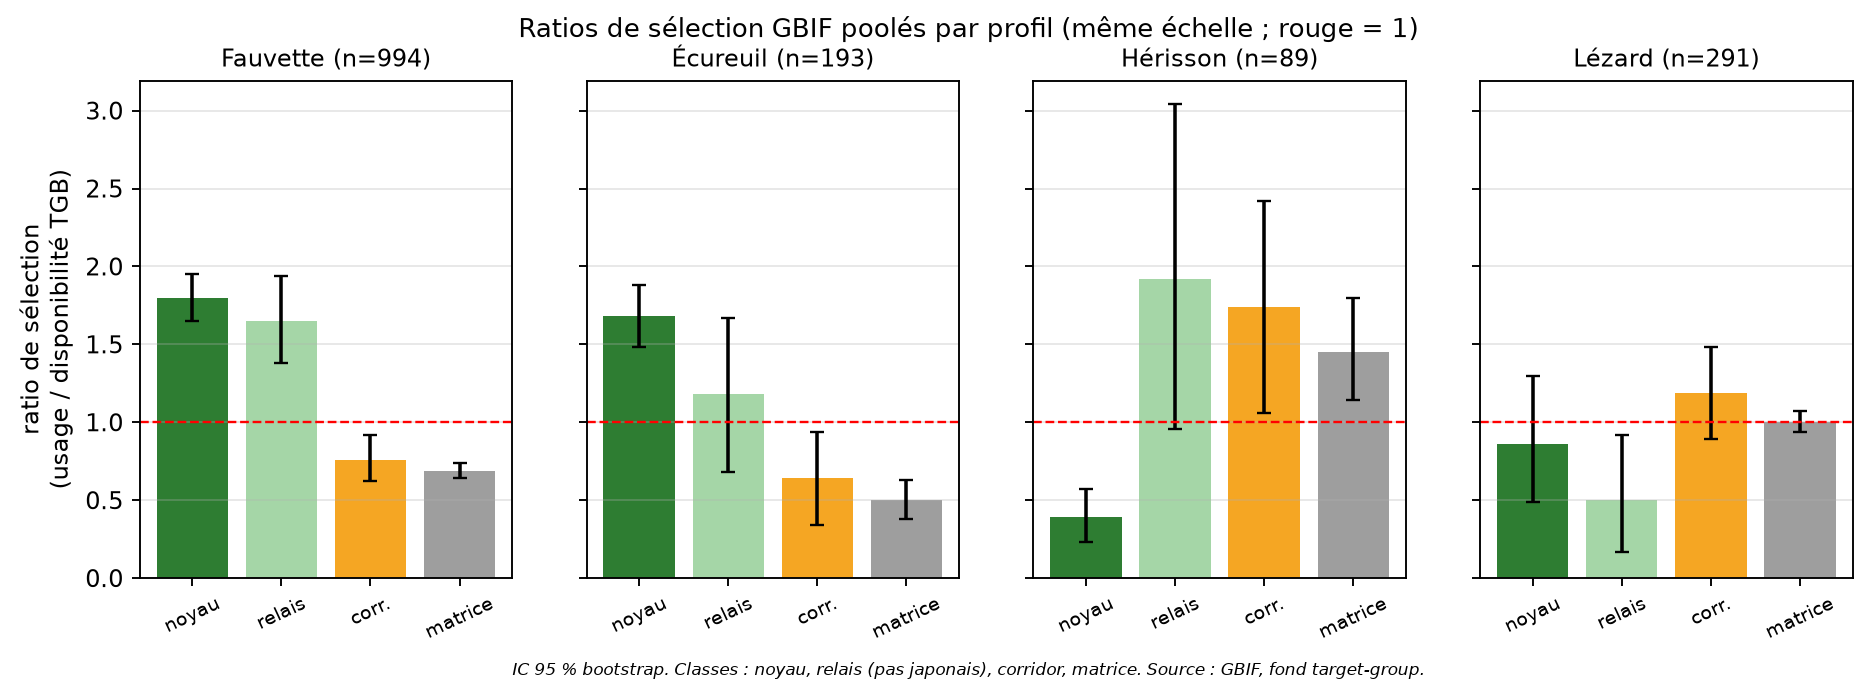
\includegraphics[width=0.98\textwidth]{figures/gbif_ratios_pooled.png}
\caption{Ratios de sélection des occurrences GBIF par profil et par classe (noyau, relais, corridor, matrice), agrégés sur les cinq territoires tempérés. (d'après les données GBIF, 2026)}
\label{fig:15}
\end{figure}

\begin{figure}[H]
\centering
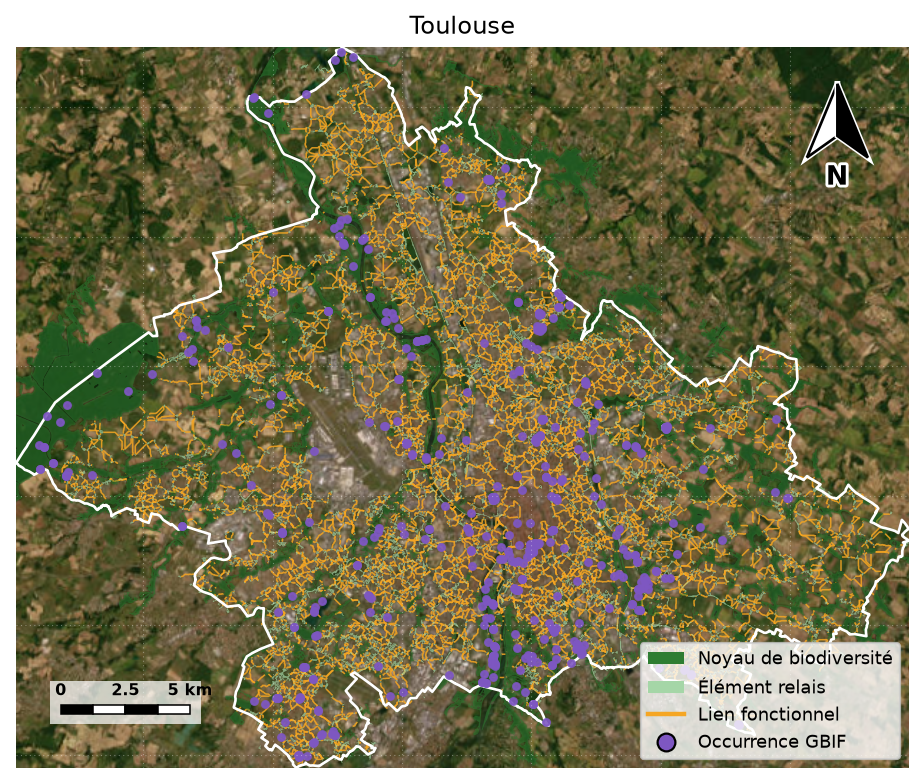
\includegraphics[width=0.98\textwidth]{figures/gbif_carte_Toulouse_fauvette.png}
\caption{Occurrences GBIF de l'oiseau de lisière à Toulouse superposées aux noyaux, espaces relais et corridors modélisés. (d'après les données GBIF, 2026)}
\label{fig:16}
\end{figure}

La seconde, la comparaison à la méthode du Cerema Dter Sud-Ouest \hyperref[sec:bibliographie]{(2025)}, porte sur La Rochelle, territoire commun aux deux démarches : les noyaux et tracés de moindre coût produits ici ont été superposés à ceux du Cerema Dter Sud-Ouest (\hyperref[fig:17]{Figure 17}). \hl{[À COMPLÉTER : quantifier le recouvrement observé (part de tracés/noyaux concordants) plutôt que de le dire qualitativement ; sinon décrire précisément les zones de coïncidence et de divergence.]}

\begin{figure}[H]
\centering
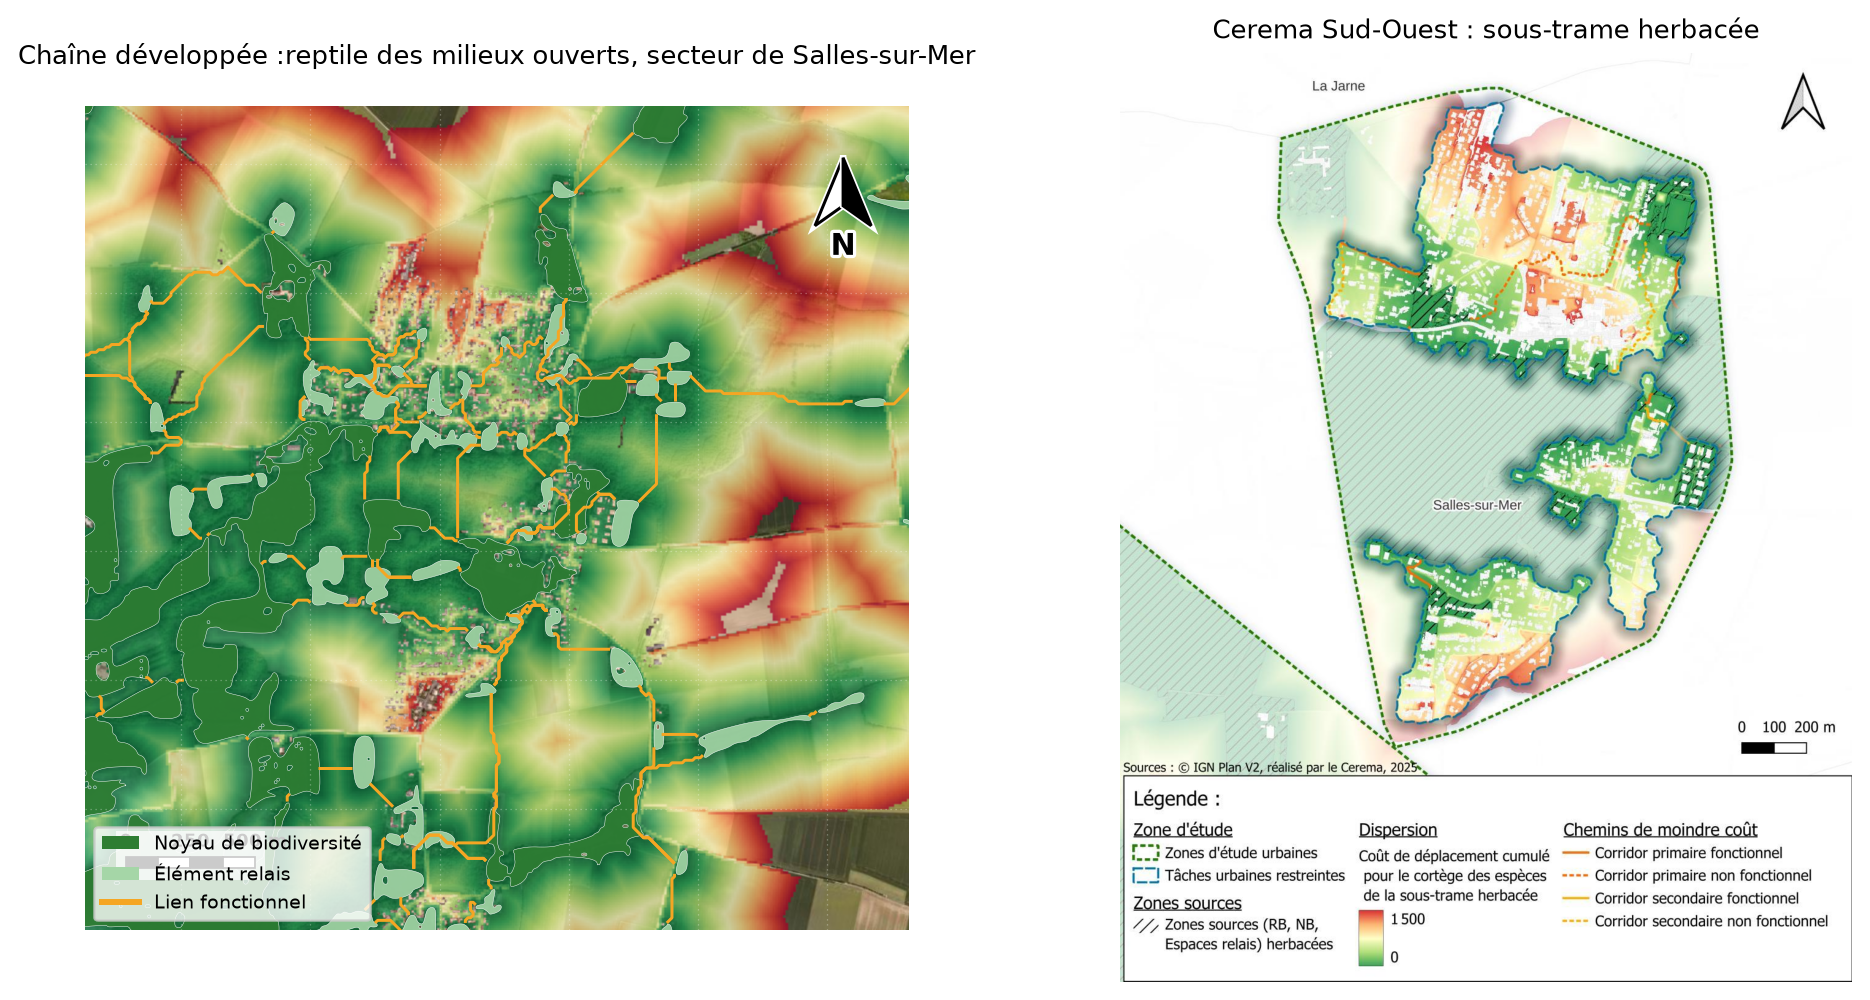
\includegraphics[width=0.98\textwidth]{figures/comparaison_salles.png}
\caption{Comparaison sur le secteur de Salles-sur-Mer, à La Rochelle (sous-trame herbacée) : méthode proposée et carte du Cerema Dter Sud-Ouest sur le même secteur. (d'après Cerema Dter Sud-Ouest, 2025)}
\label{fig:17}
\end{figure}

\section{Effet local d'un scénario de végétalisation à Toulouse}\label{sec:3.6}

Au-delà du diagnostic de l'état existant, la chaîne sert aussi d'outil prospectif : elle estime l'effet attendu d'un projet d'aménagement sur la connectivité, avant sa réalisation. C'est cette simulation avant/après qui la rapproche d'un outil d'aide à la décision, en permettant de comparer des scénarios plutôt que de seulement constater un état. Le principe est simple : le projet est intégré à l'occupation du sol comme une modification locale, puis toute la chaîne est relancée sur l'état modifié et ses sorties sont comparées à celles de l'état initial.

Ce mécanisme est illustré ici par une végétalisation de près de cinq hectares à Toulouse, le long des allées Jean-Jaurès et des ramblas : le projet est ajouté à l'occupation du sol, puis l'état avant et l'état après sont comparés à indicateurs identiques.

À l'échelle locale, la surface végétalisée devient un nouveau noyau de biodiversité que l'étape de moindre coût rattache au réseau : pour le profil de petit mammifère terrestre illustré (\hyperref[fig:18]{Figure 18}), le site passe de un à sept liens de raccordement. À l'échelle du territoire, en revanche, les indicateurs agrégés (calculés sur l'ensemble de l'emprise) sont quasiment inchangés : ils varient de moins de 0,1 \% pour les quatre profils écologiques. La surface connectée équivalente du petit mammifère terrestre passe par exemple de 7 674,2 à 7 674,6 hectares, et le nombre de sous-réseaux reste identique avant et après pour les quatre profils.

\begin{figure}[H]
\centering
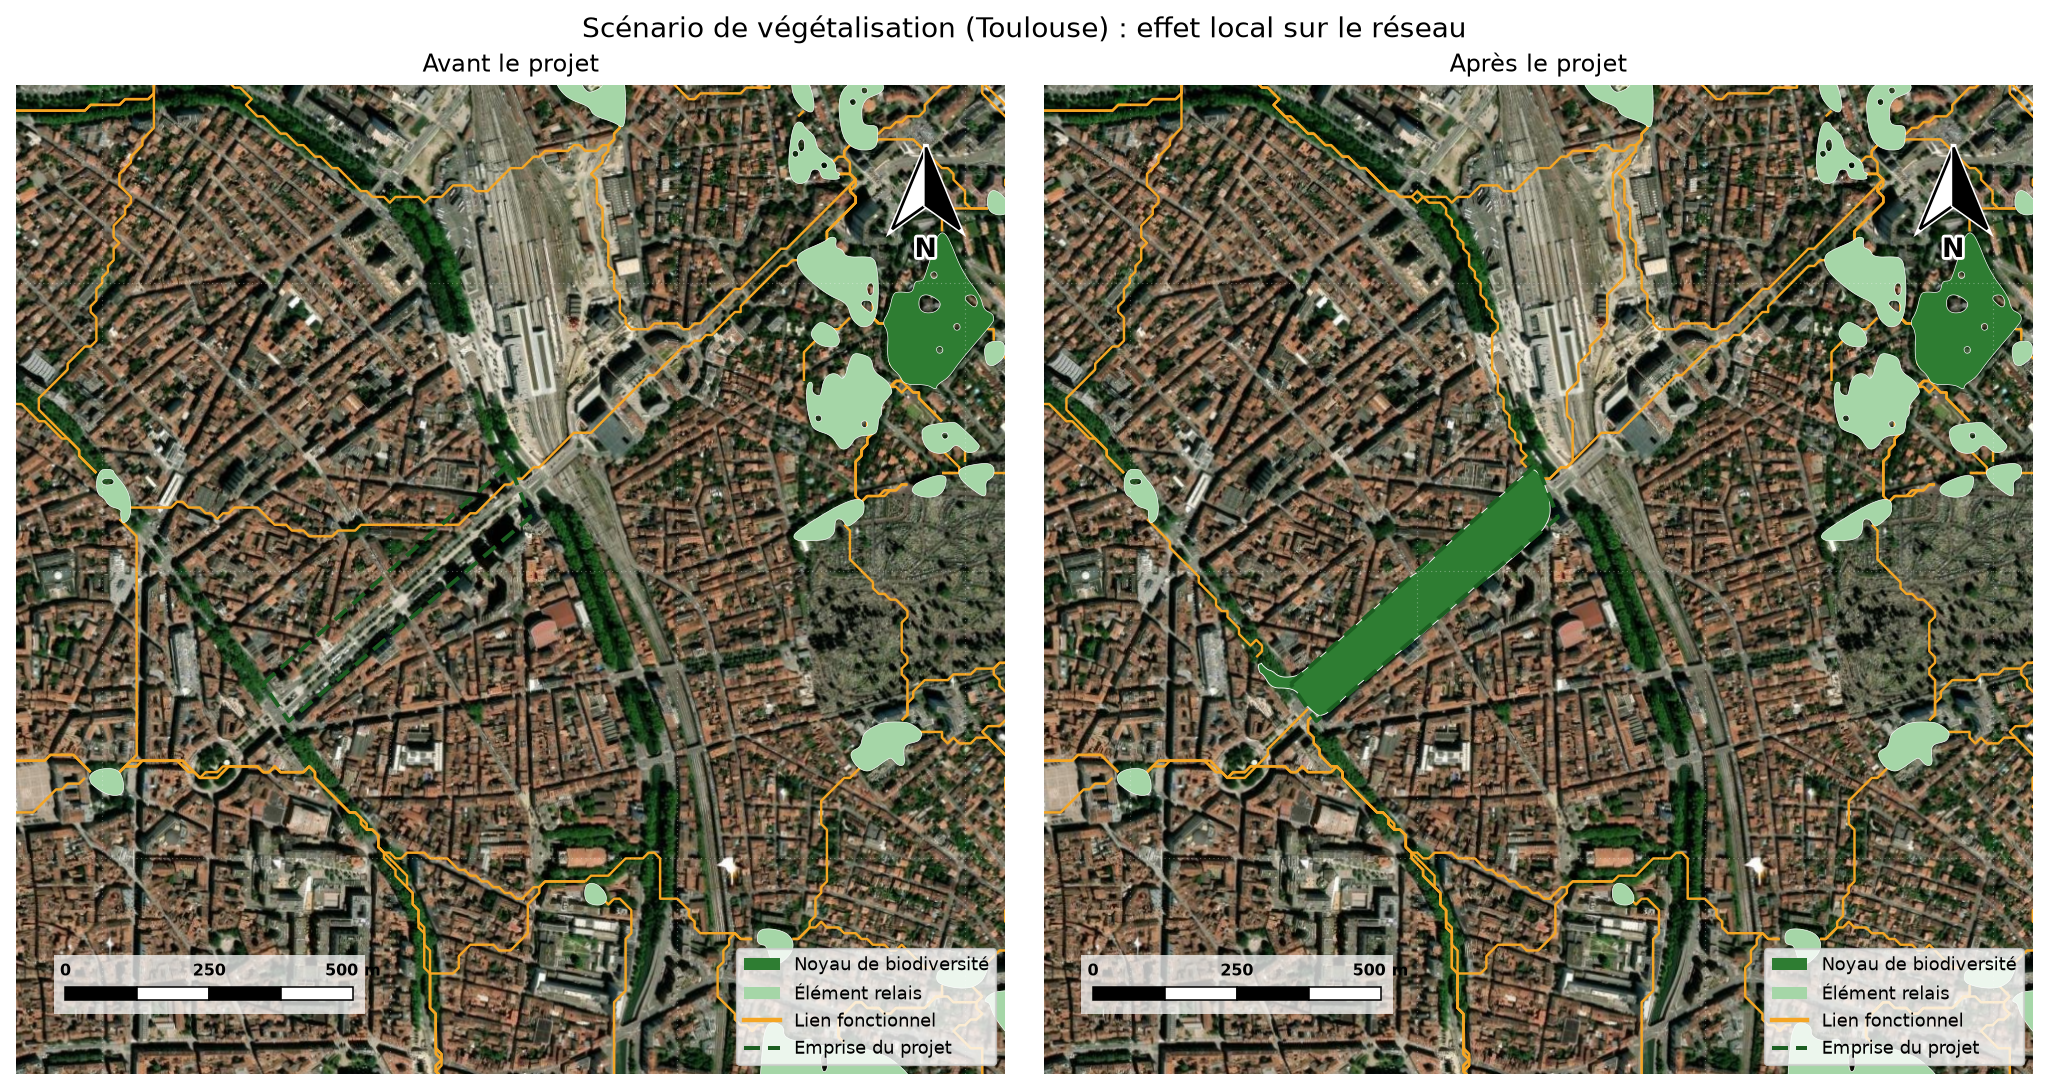
\includegraphics[width=0.98\textwidth]{figures/scenario_local.png}
\caption{Scénario de végétalisation des ramblas des allées Jean-Jaurès à Toulouse, comparaison avant/après sur le profil écologique de petit mammifère terrestre.}
\label{fig:18}
\end{figure}

\chapter{Discussion}\label{chap:4}

Ce chapitre interprète les résultats du \hyperref[chap:3]{chapitre 3} : ce que révèle une connectivité propre à chaque profil écologique (4.1), ce que la forme urbaine explique des contrastes entre territoires (4.2), ce que le scénario dit pour l'aménagement (4.3), la robustesse et la validité des sorties (4.4), l'apport opérationnel de l'outil (4.5), enfin ses limites et sa portée (4.6).

En bref, le \hyperref[chap:3]{chapitre 3} fait apparaître une connectivité fortement dépendante du profil écologique (part d'habitat connecté médiane d'environ 67 \% pour le petit mammifère terrestre, 23 \% pour le reptile), des contrastes marqués entre territoires selon la forme urbaine, un effet d'aménagement sensible localement mais négligeable à l'échelle du territoire, et des sorties qui résistent en relatif aux variations de calibration tout en restant confortées, côté habitat, par les occurrences GBIF pour les profils boisés. Les sections qui suivent en tirent les implications.

\section{Une connectivité propre à chaque profil écologique}\label{sec:4.1}

Modéliser la connectivité par profil écologique est un choix de conception, mais les résultats en confirment la portée : la connectivité dépend du profil écologique retenu et diffère nettement de l'un à l'autre. Restaurer la connectivité pour le petit mammifère terrestre, qui dispose d'une large capacité de déplacement mais pour qui les cours d'eau font obstacle, n'a pas le même sens que pour le reptile, dont l'habitat thermophile est dispersé et qui se déplace peu. En restituant quatre réseaux distincts pour un même territoire, l'outil explicite cette multiplicité et conduit à préciser pour quel profil écologique la connectivité est évaluée, là où la planification française différencie surtout par grandes strates d'habitat \hyperref[sec:bibliographie]{(sous-trames boisée, ouverte, humide ; Sordello, 2017)}, et non par capacité de déplacement des espèces. Ce constat conforte l'approche multi-espèces. Aucune espèce ne résume les besoins d'une communauté \hyperref[sec:bibliographie]{(Roberge \& Angelstam, 2004)}, et aucune ne sert de « parapluie de connectivité » universel : même les espèces les plus souvent retenues ne conviennent que dans environ 60 \% des régions \hyperref[sec:bibliographie]{(Dutta et al., 2023)}. Un jeu d'espèces aux traits contrastés vaut donc mieux qu'un choix unique \hyperref[sec:bibliographie]{(Meurant et al., 2018)}, même si empiler des réseaux mono-profils laisse de côté les interactions inter-espèces \hyperref[sec:bibliographie]{(Wood et al., 2022)}.

L'ordre observé entre profils (\hyperref[sec:3.2]{§3.2}) suit leurs traits écologiques : la chaîne restitue des différences attendues, ce qui en vérifie la cohérence interne sans valoir validation. Le meilleur classement du petit mammifère terrestre tient autant à l'étendue de son habitat qu'à sa large distance de dispersion, tandis que la fragmentation de l'oiseau de lisière, pourtant volant, s'explique par la rareté et le morcellement de l'habitat boisé plus que par sa capacité de déplacement. Ce résultat rejoint les observations, en contextes forestiers et agricoles, que les oiseaux forestiers hésitent à franchir les trouées ouvertes au-delà de quelques dizaines de mètres \hyperref[sec:bibliographie]{(Bélisle et al., 2001 ; Robertson \& Radford, 2009 ; Tremblay \& St. Clair, 2011 ; Grafius et al., 2017)}, la mobilité ne garantissant pas à elle seule la connectivité fonctionnelle des espèces volantes ; ces seuils restent toutefois dépendants de l'espèce et du contexte et ne se transposent pas mécaniquement au tissu urbain. Le rôle facilitateur des arbres épars comme relais \hyperref[sec:bibliographie]{(Robertson \& Radford, 2009)} conforte aussi l'importance des éléments relais dans la chaîne. Ce rôle déterminant de la disponibilité et de l'agencement de l'habitat rejoint le constat plus général du poids de la quantité d'habitat sur sa seule configuration \hyperref[sec:bibliographie]{(Fahrig, 2003)} et le rôle structurant de la surface des taches, que les indices de disponibilité d'habitat intègrent explicitement \hyperref[sec:bibliographie]{(Pascual-Hortal \& Saura, 2006)} et que la méta-analyse de Beninde et al. \hyperref[sec:bibliographie]{(2015)} désigne, avec la présence de corridors, comme déterminant majeur de la biodiversité intra-urbaine. Cette cohérence ne remplace pas pour autant une confrontation au mouvement réel, rarement disponible \hyperref[sec:bibliographie]{(Sawyer et al., 2011)}.

Cette concordance ne vaut cependant pas preuve : la chaîne reproduit fidèlement ce qu'elle a été paramétrée pour modéliser, et un résultat conforme aux hypothèses de calibration n'est pas, en soi, une connectivité observée. Ces sorties relèvent d'un modèle de connectivité potentielle. La part d'habitat connecté (0 à 100 \%) et la surface connectée équivalente s'interprètent en absolu, mais elles ne fixent pas de seuil écologique et ne valent pas mesure de terrain : leur usage le plus fiable est la comparaison entre profils écologiques, territoires et états d'un scénario. La surface équivalente croissant avec la taille du territoire, c'est la part connectée, normalisée, qui est privilégiée pour comparer des territoires d'emprises différentes.

\section{Des contrastes entre territoires qui reflètent la forme urbaine}\label{sec:4.2}

Les écarts de connectivité entre territoires (\hyperref[sec:3.3]{§3.3}), obtenus par une méthode identique partout, reflètent surtout la structure du paysage (la couverture d'OpenStreetMap, variable d'une ville à l'autre \hyperref[sec:bibliographie]{(Barrington-Leigh \& Millard-Ball, 2017)}, restant un facteur de confusion résiduel), ce qui fait de l'outil un instrument de comparaison des territoires eux-mêmes (\hyperref[fig:19]{Figure 19}). Une trame urbaine compacte et fortement imperméabilisée fragmente nettement les profils écologiques terrestres : les noyaux y sont petits et séparés par une matrice hostile, et les ruptures se multiplient sur le réseau routier. Cet effet de l'imperméabilisation est documenté en ville, avec une relation non linéaire \hyperref[sec:bibliographie]{(bascule de l'activité vers 60 \% de bâti chez la chauve-souris, atténuée par des réseaux arborés connectés ; Hale et al., 2012)} ; il apparaît toutefois surtout au-delà d'un seuil, une ville peu dense (imperméabilisation inférieure à environ 42 \%) pouvant ne montrer aucun effet net \hyperref[sec:bibliographie]{(Larson \& Sander, 2024)}, ce qui invite à ne pas généraliser le lien compacité-fragmentation hors des tissus les plus denses. Là où la ville conserve de grandes continuités végétalisées, coulées vertes, ceinture boisée, vallée, le réseau reste mieux structuré et les corridors s'appuient sur ces armatures. Ce rôle des armatures végétalisées rejoint les travaux montrant que des corridors boisés structurent les communautés jusque dans les villes \hyperref[sec:bibliographie]{(Vergnes et al., 2012 ; Braaker et al., 2014)}. Un cours d'eau traversant joue un rôle ambivalent : support de continuité pour les profils écologiques qui le franchissent, coupure pour ceux dont il est un obstacle. À Calgary, les rivières se sont même révélées moins perméables que les routes ou les voies ferrées pour les passereaux forestiers, même en deçà de 50 m de large \hyperref[sec:bibliographie]{(Tremblay \& St. Clair, 2009)}, ce qui rappelle qu'un cours d'eau n'est un corridor que pour les profils qui le franchissent réellement.

Ce lien entre forme urbaine et connectivité se lit directement dans les indicateurs, la part d'habitat du territoire en ordonnant les résultats. La Rochelle, la moins végétalisée (environ 20 \% de couverture d'habitat), est la plus fragmentée pour les profils boisés : l'oiseau de lisière s'y morcelle en vingt-huit sous-réseaux, le mammifère arboricole en onze. Toulouse (environ 32 \%), métropole dense, connecte encore bien le petit mammifère terrestre (52 \%) mais effondre le reptile (9 \%, huit sous-réseaux). Perpignan, compacte et méditerranéenne (environ 39 \%), fragmente surtout le reptile (quatorze sous-réseaux). À l'inverse, Nancy et La Roche-sur-Yon, plus végétalisées (environ 48 à 50 \%), conservent un réseau connexe pour le petit mammifère terrestre (71 et 83 \%). Un point mérite toutefois nuance : une forte couverture végétale totale ne garantit pas la connectivité de chaque profil. La Roche-sur-Yon, verte à 50 \%, connecte 83 \% de l'habitat du petit mammifère terrestre mais seulement 28 \% de celui de l'arboricole et 19 \% de celui de l'oiseau de lisière, l'habitat boisé y étant dispersé dans une matrice agricole ; c'est donc l'agencement de l'habitat propre à chaque profil, plus que la seule quantité de vert, qui commande la connectivité.

\begin{figure}[H]
\centering
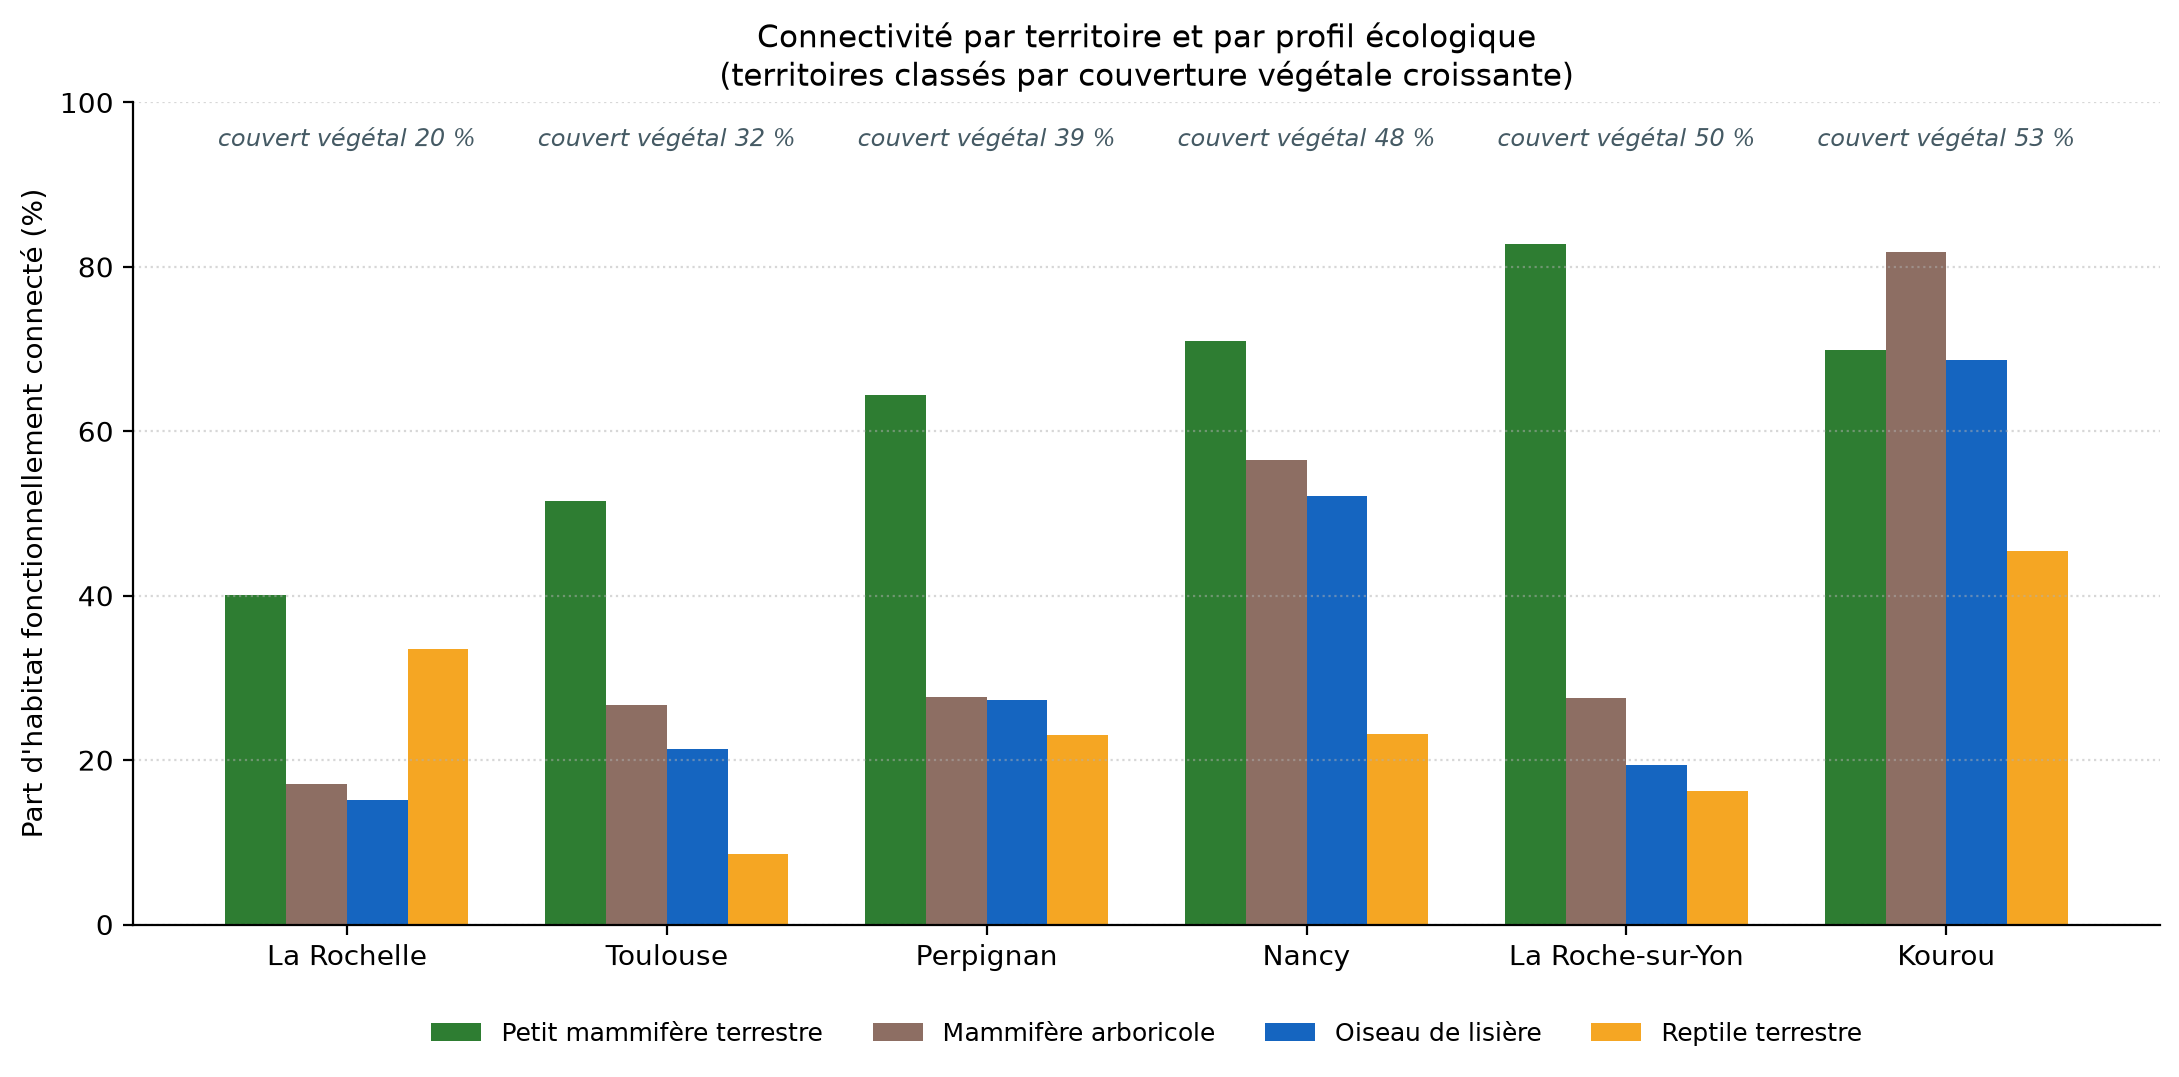
\includegraphics[width=0.98\textwidth]{figures/territoire_connectivite.png}
\caption{Part d'habitat connecté par territoire et par profil écologique, territoires classés par couverture végétale croissante. La connectivité croît globalement avec le couvert, mais l'écart entre profils au sein d'un même territoire, marqué à La Roche-sur-Yon, montre que l'agencement de l'habitat compte autant que sa quantité.}
\label{fig:19}
\end{figure}

La nature du couvert, et pas seulement son étendue, distingue les territoires. La Rochelle, littorale, est presque dépourvue de boisement (forêt sur 4,5 \% de l'emprise seulement), ce qui explique l'effondrement des profils boisés. Toulouse, métropole dense, conserve un couvert arboré modéré (20 \%) mais très peu de milieux ouverts (11 \%), d'où la fragmentation du reptile. Perpignan, méditerranéenne et compacte, combine peu de forêt (11 \%) et une matrice arbustive. Nancy est le plus forestier des territoires tempérés (33 \% de forêt), ce qui soutient la bonne connectivité du mammifère arboricole et de l'oiseau de lisière. La Roche-sur-Yon, la plus végétalisée (50 \%), l'est surtout en milieux herbacés et agricoles (forêt sur 20 \% seulement), d'où le contraste déjà noté entre un petit mammifère terrestre bien connecté et des profils boisés dispersés. Kourou, enfin, s'insère dans un couvert forestier équatorial (37 \% de forêt).

Kourou demande une lecture prudente. Ses parts connectées élevées sur tous les profils (de 45 \% pour le reptile à 82 \% pour l'arboricole, pour une couverture d'habitat d'environ 53 \%) sont cohérentes avec une petite ville insérée dans un couvert forestier quasi continu ; mais les profils écologiques tempérés y sont peu représentatifs et le besoin opérationnel y est moindre. Ce cas illustre surtout la transposabilité de la chaîne à un biome très différent, plus qu'un diagnostic écologique directement exploitable.

Cette comparaison a une valeur opérationnelle directe : elle montre qu'un même geste d'aménagement n'a pas le même effet selon le tissu urbain, et que la priorité, renforcer les espaces relais dans certains territoires, rétablir une continuité interrompue dans d'autres, dépend de la structure propre à chaque territoire.

\section{Un aménagement qui agit localement, invisible dans les indicateurs agrégés}\label{sec:4.3}

Un aménagement d'échelle urbaine courante agit localement, en créant un noyau que l'étape de moindre coût raccorde au réseau, sans déplacer les indicateurs agrégés, qui diluent un projet de quelques hectares sur l'ensemble de l'emprise : sur le cas de Toulouse (\hyperref[sec:3.6]{§3.6}), le site gagne des liens de raccordement alors que la part d'habitat connecté et le nombre de sous-réseaux du territoire restent inchangés. Pour de tels projets, c'est donc l'échelle locale qui renseigne la décision : l'indicateur global ne se déplace que pour un projet bien plus vaste, ou situé précisément sur un point de rupture du réseau dont le rétablissement reconnecte de grands ensembles. L'indicateur agrégé n'est donc pas adapté à l'évaluation de petits aménagements, ce qui oriente la lecture du tableau de bord vers le voisinage du site plutôt que vers la valeur globale de connectivité.

Cette lecture locale a une valeur opérationnelle directe : elle chiffre ce qu'un projet précis change dans son voisinage et permet d'arbitrer entre des gestes concurrents, renforcer un espace relais à un endroit, rétablir une continuité interrompue à un autre. Elle invite surtout à distinguer deux usages de l'outil : le diagnostic comparatif, à l'échelle du territoire et entre profils écologiques, et l'évaluation d'un projet, à l'échelle du site et de son voisinage immédiat, chacun appelant un indicateur et une échelle de lecture différents.

\section{Validité : vérification, validation interne, externe et de terrain}\label{sec:4.4}

La validité d'un modèle de connectivité s'apprécie sur plusieurs niveaux complémentaires. La démarche retenue ici en distingue quatre et situe le travail sur chacun, plutôt que de le déclarer globalement valide ou non. La vérification porte sur l'implémentation, à savoir si le code calcule correctement les indices annoncés : les formules retenues sont celles de la littérature (équations (1) à (4)) et le contrôle automatisé des sorties (\hyperref[chap:2]{chapitre 2}) écarte les erreurs grossières, mais un étalonnage formel contre un logiciel de référence (Graphab, Conefor) reste à mener et serait peu coûteux sur un cas test. La validation interne examine la sensibilité au paramétrage (\hyperref[sec:3.4]{§3.4}). La validation externe confronte les sorties à une méthode indépendante, celle du Cerema Dter Sud-Ouest appliquée à La Rochelle \hyperref[sec:bibliographie]{(2025)}, et à des observations d'espèces (GBIF, \hyperref[sec:3.5]{§3.5}). La validation de terrain, enfin, une confrontation à des données de mouvement ou d'occurrence suivies, sort du périmètre du stage ; les coefficients de friction et les distances de dispersion sont toutefois empruntés à des études elles-mêmes validées sur le terrain \hyperref[sec:bibliographie]{(Balbi et al., 2019, 2021)}, de sorte que des paramètres validés ailleurs sont ici transférés, au prix d'une hypothèse à assumer : que le comportement mesuré à Rennes ou Zurich vaille dans les villes étudiées. Les paragraphes suivants précisent où en est le travail sur chacun de ces niveaux.

La robustesse aux choix de calibration (\hyperref[sec:3.4]{§3.4}) indique que les conclusions comparatives, entre profils et entre territoires, résistent à une variation plausible des frictions et des distances de dispersion, tandis que les valeurs absolues (part connectée, surface équivalente) en dépendent directement. Cette robustesse reste toutefois conditionnelle, la sensibilité des graphes de moindre coût aux valeurs relatives de coût étant maximale précisément dans les paysages fragmentés à matrice intermédiaire \hyperref[sec:bibliographie]{(Rayfield et al., 2010)}, configuration proche de plusieurs des territoires étudiés. Le reptile, peu mobile et à l'habitat rare, se tient près d'un point de bascule au-delà duquel son réseau se scinde en plusieurs sous-réseaux, quand le généraliste en reste loin ; un territoire déjà morcelé rapproche d'autant chaque profil de ce basculement. La connectivité tient au contraste entre frictions plus qu'à leur niveau absolu, ce qui désigne l'écart de résistance entre classes d'occupation du sol comme le paramètre déterminant, en cohérence avec l'observation, faite en théorie des circuits, que le rang des résistances importe davantage que leur amplitude absolue \hyperref[sec:bibliographie]{(Bowman et al., 2020)}.

La convergence avec la méthode du Cerema Dter Sud-Ouest sur La Rochelle (2025, \hyperref[sec:3.5]{§3.5}), obtenue indépendamment à partir de données et d'outils différents, constitue une validation croisée partielle : deux démarches construites séparément aboutissent au même diagnostic là où elles se recouvrent. Cette prudence est justifiée, car des méthodes structurelles distinctes peuvent converger entre elles tout en s'écartant fortement de la connectivité fonctionnelle observée \hyperref[sec:bibliographie]{(recouvrement d'environ 21 \% avec des trajets GPS dans Rezvani et al., 2024)} ; la validation empirique reste d'ailleurs rarement réalisée en cartographie de connectivité \hyperref[sec:bibliographie]{(Laliberté \& St-Laurent, 2020)}.

La concordance avec les occurrences GBIF (\hyperref[sec:3.5]{§3.5}) valide la couche d'habitat pour les espèces d'habitat boisé, nettement sur-représentées dans les noyaux ; elle reste indicative pour le petit mammifère terrestre, généraliste tolérant à la matrice, dont la distribution urbaine est mieux captée par les éléments relais que par les grands noyaux, et non concluante pour le reptile, faute d'occurrences suffisantes. Ces données renseignent la présence, non le flux : elles confirment l'habitat, non la connectivité elle-même, la distinction entre connectivité structurelle et fonctionnelle restant le verrou central du champ \hyperref[sec:bibliographie]{(LaPoint et al., 2015 ; Habrich \& Fahrig, 2025)} ; la favorabilité d'habitat est du reste un mauvais indicateur de la connectivité au moment de la dispersion, des milieux peu favorables pouvant porter des routes de déplacement réelles \hyperref[sec:bibliographie]{(Keeley et al., 2017)}. La reproductibilité, enfin, tient au caractère déterministe de la chaîne et à son appui sur les seules données ouvertes, un tiers pouvant la rejouer de bout en bout.

Une validation de terrain reste nécessaire pour passer d'une connectivité potentielle à une connectivité vérifiée ; sa forme possible et ses limites sont exposées en perspective (\hyperref[chap:5]{chapitre 5}). À la différence des rares travaux ayant confronté des tracés de moindre coût à des mouvements réels, par translocation et recapture \hyperref[sec:bibliographie]{(Balbi et al., 2019, 2021)}, ou la résistance paysagère au flux de gènes \hyperref[sec:bibliographie]{(Beninde et al., 2016 ; Braaker et al., 2017)}, la présente chaîne repose sur des données ouvertes sans relevé de terrain ; sa validation demeure donc indirecte, ce qui situe sa portée sans l'invalider.

\section{Un apport opérationnel : l'assemblage de briques établies}\label{sec:4.5}

La contribution de ce travail est opérationnelle. Les briques employées, segmentation morphologique, graphes de connectivité, Probability of Connectivity, chemins de moindre coût, sont établies et documentées (\hyperref[chap:1]{chapitre 1}) ; l'apport vient de leur assemblage. La chaîne les réunit en un enchaînement unique, fondé sur les seules données ouvertes, décliné par profil écologique et transposable sans calibration locale, dont les sorties sont restituées à des aménageurs non spécialistes par un tableau de bord. Sa valeur tient à la reproductibilité et à l'accessibilité de l'ensemble. L'outil passe ainsi d'un diagnostic à un instrument d'aide à la décision : le test de scénarios permet d'évaluer un projet avant de le décider.

L'outil privilégie la portabilité et le faible coût à la finesse écologique : des profils génériques, l'absence de calibration de terrain et des données mondiales sont à la fois ce qui le rend applicable partout et ce qui en limite la précision écologique. Une étude locale calibrée sur des données d'occurrence et un dire d'expert serait plus juste, mais ni généralisable ni rejouable à faible coût. L'outil occupe délibérément la place d'un pré-diagnostic généralisable plutôt que d'une expertise locale, répondant à une demande opérationnelle, de nombreuses villes à traiter avec des moyens limités, plutôt qu'à une exigence académique de précision sur un site unique. Ce positionnement répond au constat récurrent d'un déficit d'outils opérationnels et validés en connectivité urbaine \hyperref[sec:bibliographie]{(LaPoint et al., 2015 ; Habrich \& Fahrig, 2025)} et rejoint les démarches récentes d'aide à la planification par groupes d'espèces \hyperref[sec:bibliographie]{(Kirk et al., 2023)}, les chaînes reproductibles sur données d'observation de la Terre déployées à l'échelle de nombreuses villes \hyperref[sec:bibliographie]{(Borghi et al., 2026, sur vingt-huit capitales européennes)} et les systèmes d'aide à la décision conçus pour des planificateurs non spécialistes \hyperref[sec:bibliographie]{(Losada-Iglesias et al., 2024)}.

La restitution conditionne enfin la réception opérationnelle. Le tableau de bord n'affiche pas toutes les couches produites : les liens jugés non fonctionnels ne sont pas représentés, pour ne pas suggérer des connexions qui n'existent pas ; les points de rupture sur l'eau, à l'inverse, sont conservés, car ils signalent des coupures sur lesquelles un aménageur peut agir. Ces choix d'affichage orientent en partie les priorités d'action ; ils sont donc explicités et justifiés dans ce rapport. Une carte de connectivité signale où la continuité est en jeu, mais elle n'est pas un acte de planification : la traduire en décision suppose un arbitrage avec d'autres enjeux urbains, que l'outil ne remplace pas.

\section{Limites et portée des résultats}\label{sec:4.6}

Les limites présentées ici n'ont pas pu être levées dans les six mois du stage. Celles qui ouvrent une suite possible sont reprises comme perspectives au \hyperref[chap:5]{chapitre 5}, plutôt que listées comme des manques. Chacune est examinée sous deux angles : le sens du biais qu'elle introduit, et le fait qu'elle pèse surtout sur la valeur absolue de l'indicateur, moins sur son usage comparatif.

Plusieurs limites conduisent à surestimer la connectivité. La couche d'occupation du sol décrit un couvert vu du ciel, sans hauteur : une canopée surplombant une surface imperméable est lue comme un habitat arboré au sol, ce qui crée des habitats fictifs, surtout dans les centres denses, et fait voir des continuités qui n'existent pas pour les profils écologiques terrestres. Une occupation du sol sans hauteur surestime effectivement la connectivité du vert urbain, le biais étant maximal pour les faibles capacités de dispersion, car toutes les strates verticales y sont traitées comme connectées \hyperref[sec:bibliographie]{(Casalegno et al., 2017)}. Dans le même sens, les obstacles fins du tissu urbain (clôtures, murs, glissières) ne figurent dans aucune donnée ouverte exploitable et ne sont pas modélisés, alors qu'ils coupent réellement les déplacements au sol : leur absence laisse passer des liens qui, sur le terrain, seraient rompus. De fait, aucun inventaire géospatial systématique des clôtures n'existe \hyperref[sec:bibliographie]{(Poor et al., 2014)}, ce qui rend ce biais structurellement difficile à corriger à partir de données ouvertes.

L'incidence de la résolution est plus ambiguë. À 10 m, les éléments fins du paysage (haies étroites, alignements d'arbres, petits jardins) passent sous le seuil de détectabilité de Sentinel-2 \hyperref[sec:bibliographie]{(Radoux et al., 2016)} et disparaissent, ce qui fait perdre des relais et tend à sous-estimer la connectivité ; mais à la même résolution, une coupure étroite (route ou bande bâtie plus fine que le pixel) peut être absorbée dans une classe végétalisée dominante et souder artificiellement deux taches, ce qui surestime au contraire la continuité. La perte de ces petits éléments n'est en outre pas seulement un défaut : elle écarte aussi les micro-taches trop petites pour constituer un habitat fonctionnel, tel un arbre isolé, qui seraient sinon comptées à tort comme noyaux ou relais. La direction du biais lié à la résolution n'est donc pas tranchée et dépend de la configuration locale.

Ces biais jouent en sens contraires, et parfois indéterminés ; ils ne se compensent pas de façon prévisible, et leur effet net sur une valeur absolue de connectivité reste inconnu. C'est pourquoi l'indicateur n'est exploité qu'en relatif : tant que les mêmes biais s'appliquent à tous les profils écologiques, à tous les territoires et aux deux états d'un scénario, la comparaison les neutralise en grande partie, quand la valeur absolue, elle, demeure peu fiable. Cette lecture relative a toutefois sa propre limite : elle suppose que les biais s'appliquent uniformément, or certains ne le sont pas, la confusion de la canopée sur surface imperméable étant par exemple plus fréquente dans les centres denses qu'en périphérie ; une comparaison entre deux secteurs très contrastés d'un même territoire peut donc rester affectée.

À ces biais s'ajoute une dépendance à la calibration. Les valeurs de friction et les distances de dispersion proviennent de la table du Cerema Dter Sud-Ouest, elle-même construite à partir de plusieurs sources (littérature, dires d'expert, données locales), puis sont réinterprétées et ajustées ici (\hyperref[chap:2]{chapitre 2}) ; l'analyse de sensibilité (\hyperref[sec:3.4]{§3.4}) montre que les classements entre profils et entre territoires restent stables lorsqu'on fait varier ces paramètres dans une plage plausible, quand les valeurs absolues, elles, varient, ce qui renforce le statut d'indice relatif des sorties. Chaque profil écologique est en outre défini par les paramètres d'une espèce repère, et les quatre profils retenus ne couvrent qu'imparfaitement la diversité fonctionnelle : le profil des insectes, un temps envisagé, a été écarté faute d'une occupation du sol assez fine à 10 m pour distinguer leurs micro-habitats, et les pollinisateurs comme les petits invertébrés ne sont pas représentés. Les réseaux produits valent pour les profils de déplacement retenus, non pour l'ensemble de la faune urbaine.

D'autres limites n'affectent pas tant la valeur que son interprétation. La qualité estimée des noyaux est structurelle, fondée sur la taille et la compacité, et non écologique : les pressions diffuses \hyperref[sec:bibliographie]{(pollution lumineuse, Gaston et al., 2013 ; pollution sonore, Francis \& Barber, 2013 ; prédation par le chat domestique, Loss et al., 2013 ; dérangement, gestion des espaces)} ne sont pas captées, si bien qu'un grand noyau compact peut recouvrir un habitat dégradé. L'intensité du trafic n'est pas davantage prise en compte, une route pesant par sa classe et non par son flux. Ces mêmes pressions sensorielles, éclairage et bruit, agissent en outre comme des barrières au déplacement qu'une carte d'occupation du sol ne capte pas : le modèle les ignore et surestime d'autant la perméabilité du tissu urbain. Le tracé des chemins de moindre coût est aussi approximatif pour tous les profils et tous les territoires. L'occupation du sol, qui fusionne WorldCover et OpenStreetMap, est ramenée à une grille de dix mètres attribuant une seule classe par pixel, alors qu'un pixel de dix mètres est souvent mixte sur le terrain. Un pixel classé perméable peut ainsi contenir un bâtiment que sa classe n'indique pas, franchi sans le voir par un chemin de moindre coût, tandis qu'un pixel réellement classé comme bâti reste, lui, correctement infranchissable. Le calcul sur une grille à huit directions, puis le lissage cartographique appliqué aux lignes, accentuent ce caractère : la géométrie précise d'un corridor doit donc être lue comme indicative, à l'échelle du tissu urbain, et non au mètre près, sans que cela change les liens du réseau ni leur coût. Un lien peut ainsi sembler traverser un bâtiment, soit que celui-ci occupe un pixel non codé comme bâti, soit que le lissage ait rogné un angle : le tracé vaut indication et non itinéraire de terrain, et appelle une vérification locale avant tout usage fin. Les sorties décrivent enfin des potentialités à une date donnée, celle de l'imagerie, sans dynamique saisonnière ni temporelle, alors que la connectivité fonctionnelle est souvent intermittente, s'ouvrant par fenêtres selon les conditions de la matrice \hyperref[sec:bibliographie]{(Zeigler \& Fagan, 2014)}. Cette limite est en partie tempérée par le caractère rejouable de la chaîne : construite sur des données ouvertes régulièrement mises à jour, elle peut être relancée sur les millésimes ultérieurs d'occupation du sol pour suivre l'évolution dans le temps.

La limite la plus structurante reste l'absence de validation de terrain : faute de données d'occurrence ou de suivi, les sorties demeurent des potentialités et non une connectivité observée, ce qui marque la frontière de ce qu'une approche fondée sur des données ouvertes et sans relevé de terrain peut affirmer. À cette limite pratique s'ajoute une limite de principe : le déplacement animal comporte une part aléatoire qu'un modèle déterministe à chemin unique ne restitue pas ; le mouvement réel se situe en fait entre l'optimum du moindre coût et la marche aléatoire de la théorie des circuits \hyperref[sec:bibliographie]{(Panzacchi et al., 2016)}, de sorte que la connectivité modélisée décrit une potentialité et non un comportement certain. Le périmètre reste volontairement limité à la trame verte : la trame bleue et la connectivité aquatique en sont exclues, d'où l'absence de profil écologique amphibie, alors même que les amphibiens comptent parmi les groupes les plus menacés par la fragmentation et l'urbanisation \hyperref[sec:bibliographie]{(Cushman, 2006 ; Hamer \& McDonnell, 2008)} ; ce manque est repris comme perspective au \hyperref[chap:5]{chapitre 5}.

Ces limites dessinent deux directions d'erreur symétriques, qu'aucune donnée de terrain ne permet ici de chiffrer. Le modèle peut surestimer la connectivité (faux positifs) en traçant un corridor là où le déplacement n'a pas lieu, faute d'avoir vu une pression sensorielle ou un trafic intense. Il peut à l'inverse la sous-estimer (faux négatifs) en annonçant une rupture là où un passage à faune non recensé, ou une haie et des jardins sous la résolution de dix mètres, assurent en réalité la continuité.

Ces limites ne rendent pas l'outil inutilisable : elles en circonscrivent l'usage. C'est un instrument reproductible et peu coûteux de pré-diagnostic comparatif, qui signale où la connectivité est vraisemblablement en jeu et permet de simuler plusieurs scénarios d'aménagement et de les comparer, et non un substitut à une étude écologique de terrain là où les enjeux sont forts.

\chapter{Conclusion et perspectives}\label{chap:5}

\section{Conclusion}\label{sec:5.1}

Ce travail construit et teste une preuve de concept : une chaîne reproductible qui cartographie la connectivité écologique urbaine à partir de la seule observation de la Terre et de données ouvertes, en réponse au verrou identifié en introduction, celui d'outils de connectivité puissants mais experts et peu transposables. Les cinq objectifs fixés en ont structuré la construction.

La chaîne conduit de bout en bout des données ouvertes, WorldCover et OpenStreetMap, jusqu'aux composantes des continuités écologiques potentielles : noyaux de biodiversité, espaces relais, liens fonctionnels, points de rupture et surfaces de dispersion. Elle a produit vingt-quatre jeux de sorties normalisés, six territoires par quatre profils écologiques, tous directement exploitables en système d'information géographique comme dans le tableau de bord.

Le raisonnement s'appuie sur des profils écologiques, dont les paramètres de friction et de dispersion proviennent de l'étude du Cerema et des travaux qu'elle agrège, puis sont réinterprétés au niveau du syndrome de déplacement, plutôt que par une espèce focale unique. Elle restitue ainsi quatre réseaux distincts pour un même territoire, là où une trame verte indifférenciée laisserait invisibles des besoins de continuité propres à chaque capacité de déplacement : la part d'habitat connecté s'échelonne de moins de 10 \% pour le reptile à Toulouse à plus de 80 \% pour le petit mammifère terrestre à La Roche-sur-Yon.

Implémentée intégralement en Python, sans recours aux logiciels spécialisés existants, elle est automatisable et déterministe, sans composante aléatoire : une même commande régénère l'ensemble des résultats d'un territoire, et sa reproduction à l'identique ne requiert que les données publiques et un fichier de configuration.

Ses sorties sont restituées dans un tableau de bord interactif destiné à des aménageurs non spécialistes, qui permet d'explorer le réseau d'un territoire, d'en superposer les couches et de comparer l'effet de scénarios d'aménagement.

La chaîne a enfin été exécutée, sans aucun réglage local, sur six territoires aux contextes bioclimatiques contrastés, de la façade atlantique à la Guyane équatoriale, premier test de sa transposabilité.

La contribution est ainsi opérationnelle plus que théorique : elle réside dans l'assemblage de briques établies en une chaîne unique et accessible, prolongée jusqu'à une sortie directement exploitable et au test de scénarios. Ces résultats relèvent d'un modèle de connectivité potentielle : ils signalent où la connectivité est vraisemblablement en jeu et permettent de simuler plusieurs scénarios d'aménagement et de les comparer. Ils ont la portée d'un pré-diagnostic, rapide et peu coûteux, à confirmer par des études de terrain avant toute décision.

\section{Perspectives}\label{sec:5.2}

Le principal prolongement porte sur la validation. Le faisceau de vérifications présenté au \hyperref[chap:4]{chapitre 4} (sensibilité, comparaison à la méthode du Cerema Dter Sud-Ouest sur La Rochelle, occurrences GBIF, reproductibilité) gagnerait à être complété par un protocole de terrain. Un plan d'échantillonnage stratifié opposerait des secteurs témoins, éloignés de toute coupure, à des secteurs proches d'une infrastructure fragmentante, le nombre de relevés par strate étant dimensionné à l'avance, par un calcul de puissance statistique, de manière à pouvoir détecter un écart d'occupation donné. Les corridors modélisés seraient échantillonnés en priorité, afin de tester s'ils sont effectivement empruntés. Plusieurs méthodes se combineraient selon le profil écologique : relevés d'occurrence et pièges photographiques pour l'usage des passages, radio-pistage ou génétique du paysage \hyperref[sec:bibliographie]{(Spear et al., 2010)} pour le mouvement lui-même. Une telle validation reste coûteuse et se heurte à la part non déterministe du déplacement animal, mais c'est elle qui ferait passer l'outil d'une connectivité potentielle à une connectivité vérifiée.

L'enrichissement des données d'entrée ouvrirait ensuite de nouveaux usages, chacun comblant une limite identifiée de la chaîne actuelle.

L'extension à la trame bleue, avec l'introduction d'un profil écologique amphibie, comblerait la principale lacune de périmètre. Le réseau hydrographique (cours d'eau, plans d'eau, zones humides) n'est aujourd'hui pas traité comme une sous-trame à part entière, alors que les amphibiens comptent parmi les groupes les plus sensibles à la fragmentation \hyperref[sec:bibliographie]{(Cushman, 2006 ; Hamer \& McDonnell, 2008)} et à la mortalité routière \hyperref[sec:bibliographie]{(Hels \& Buchwald, 2001)}, et dépendent de continuités terre-eau qui leur sont propres.

Une donnée sur la nature du sol sous le couvert végétal lèverait une ambiguïté de l'occupation du sol optique : vue du ciel, une canopée reçoit la même classe qu'elle surplombe un sol végétalisé ou une surface imperméable, alors que la valeur écologique des deux diffère fortement, un arbre isolé au-dessus d'un trottoir bitumé n'étant pas un habitat. Une couche d'imperméabilisation des sols distinguerait ces deux cas ; un modèle de hauteur de végétation, de type LiDAR, y ajouterait la séparation entre végétation basse et couvert arboré.

L'intensité du trafic routier permettrait de pondérer l'effet fragmentant des voies au-delà de leur seule catégorie : à classe égale, une route très circulée forme une barrière plus forte qu'une route peu fréquentée.

Enfin, l'adossement des franchissements à des ouvrages réels (passages à faune, buses et ponts recensés) ferait passer les tracés de moindre coût là où un franchissement est physiquement possible, plutôt qu'au seul point de moindre coût théorique. La base nationale SIPAF (Système d'information sur les passages à faune) a été envisagée à cette fin, mais elle demeure incomplète et ne recense aucun ouvrage dans les emprises étudiées.

Une dimension sensorielle reste enfin hors de ce périmètre purement structurel. Le déplacement de la faune est aussi entravé par des barrières absentes d'une carte d'occupation du sol : la pollution lumineuse, qui perturbe les espèces nocturnes (trame noire), et la pollution sonore, qui repousse les espèces sensibles au bruit (trame blanche). Le groupe de travail du Cerema sur les différents types de trames traite explicitement ces pressions dans le cadre d'UrbiVerde ; la chaîne pourrait les intégrer comme couches de résistance supplémentaires, la pollution lumineuse étant par exemple cartographiable par la radiance nocturne du capteur VIIRS (Visible Infrared Imaging Radiometer Suite), la pollution sonore par les cartes de bruit stratégiques ou l'intensité du trafic.

La nature reproductible de la chaîne la destine enfin à un déploiement à plus grande échelle. Testée sur six territoires, elle peut être appliquée à beaucoup d'autres pour un coût marginal quasi nul, et s'insérer dans les processus de planification des gestionnaires d'infrastructures vertes, au sein de la plateforme UrbiVerde à laquelle elle a vocation à fournir le service dédié aux continuités écologiques.

\chapter{Retour d'expérience}\label{chap:6}

\section{Conduite de projet}\label{sec:6.1}

En début de stage, une phase d'appropriation du domaine a précédé la conception : j'ai suivi le MOOC « Trame verte et bleue » de l'Office français de la biodiversité pour m'approprier le cadre réglementaire et les enjeux de continuité écologique avant d'entrer dans la partie technique. En cours de stage, j'ai également assisté au webinaire « MitiConnect : retours d'expérience » de l'OFB, le 5 juin 2026, consacré aux usages de cet outil de modélisation de la trame verte, proche de la démarche développée ici.

Les pistes envisagées en début de stage décrivaient un outil au périmètre étendu : une occupation du sol produite par apprentissage profond sur séries temporelles Sentinel-2 et plusieurs capteurs complémentaires, des profils écologiques, une modélisation combinant graphe, moindre coût et théorie des circuits, des cartes de consensus entre profils écologiques, un ensemble d'indicateurs agrégés par zone administrative, une suggestion d'élargissement des réservoirs et l'estimation de co-bénéfices climatiques. Compte tenu du temps d'un stage et de l'exigence de reproductibilité sur des biomes contrastés, ce périmètre a été délibérément resserré vers une première version fonctionnelle, cohérente et transférable.

Ce recentrage est un choix d'ingénierie : livrer un socle qui fonctionne de bout en bout, à limites connues, plutôt qu'un ensemble plus large mais inabouti. Les éléments mis de côté (classification d'occupation du sol sur mesure, théorie des circuits, métriques d'importance, co-bénéfices, scores par zone) sont repris comme perspectives au \hyperref[chap:5]{chapitre 5} ; les choix internes à ce périmètre sont détaillés à la section suivante.

Une fois obtenus les résultats sur les quatre villes pilotes, Toulouse a été ajoutée comme cas de contrôle. Je connais bien ce territoire, ce qui m'a permis de vérifier visuellement que les composantes produites, infrastructures fragmentantes, passages de biodiversité et habitats, y correspondaient à la réalité de terrain. La chaîne s'étant révélée simple à étendre à un nouveau territoire, La Rochelle a ensuite été ajoutée lorsque la découverte de la méthode du Cerema, auprès de Vanessa Rauel, en a fait un territoire de comparaison.

Le rapprochement du planning prévisionnel et du planning réalisé (\hyperref[fig:20]{Figure 20}) fait apparaître un décalage entre le prévu et le réalisé. Les simplifications de méthode ont allégé le début du stage : renoncer à une classification d'occupation du sol sur mesure au profit de WorldCover complété par OpenStreetMap a raccourci la phase technique et servi l'objectif de reproductibilité. Le temps ainsi dégagé a été absorbé par la fiabilisation et l'optimisation de la chaîne, plus longues que prévu : la stabilisation du pipeline, de la désynchronisation des identifiants de n\oe{}uds au graphe construit sur des géométries invalides, en passant par les points de rupture et le lissage des n\oe{}uds ramené de plusieurs heures à quelques secondes, s'est étendue sur le mois de juin, au-delà du jalon de finalisation initialement fixé à la mi-juin. L'analyse de sensibilité, modeste au prévisionnel, est devenue une campagne de calcul à part entière en juillet. La rédaction des résultats et de la discussion, prévue au printemps, s'est en conséquence concentrée sur la fin du stage, une fois les sorties figées, la production des figures et des cartes intervenant en dernier.

\begin{figure}[H]
\centering
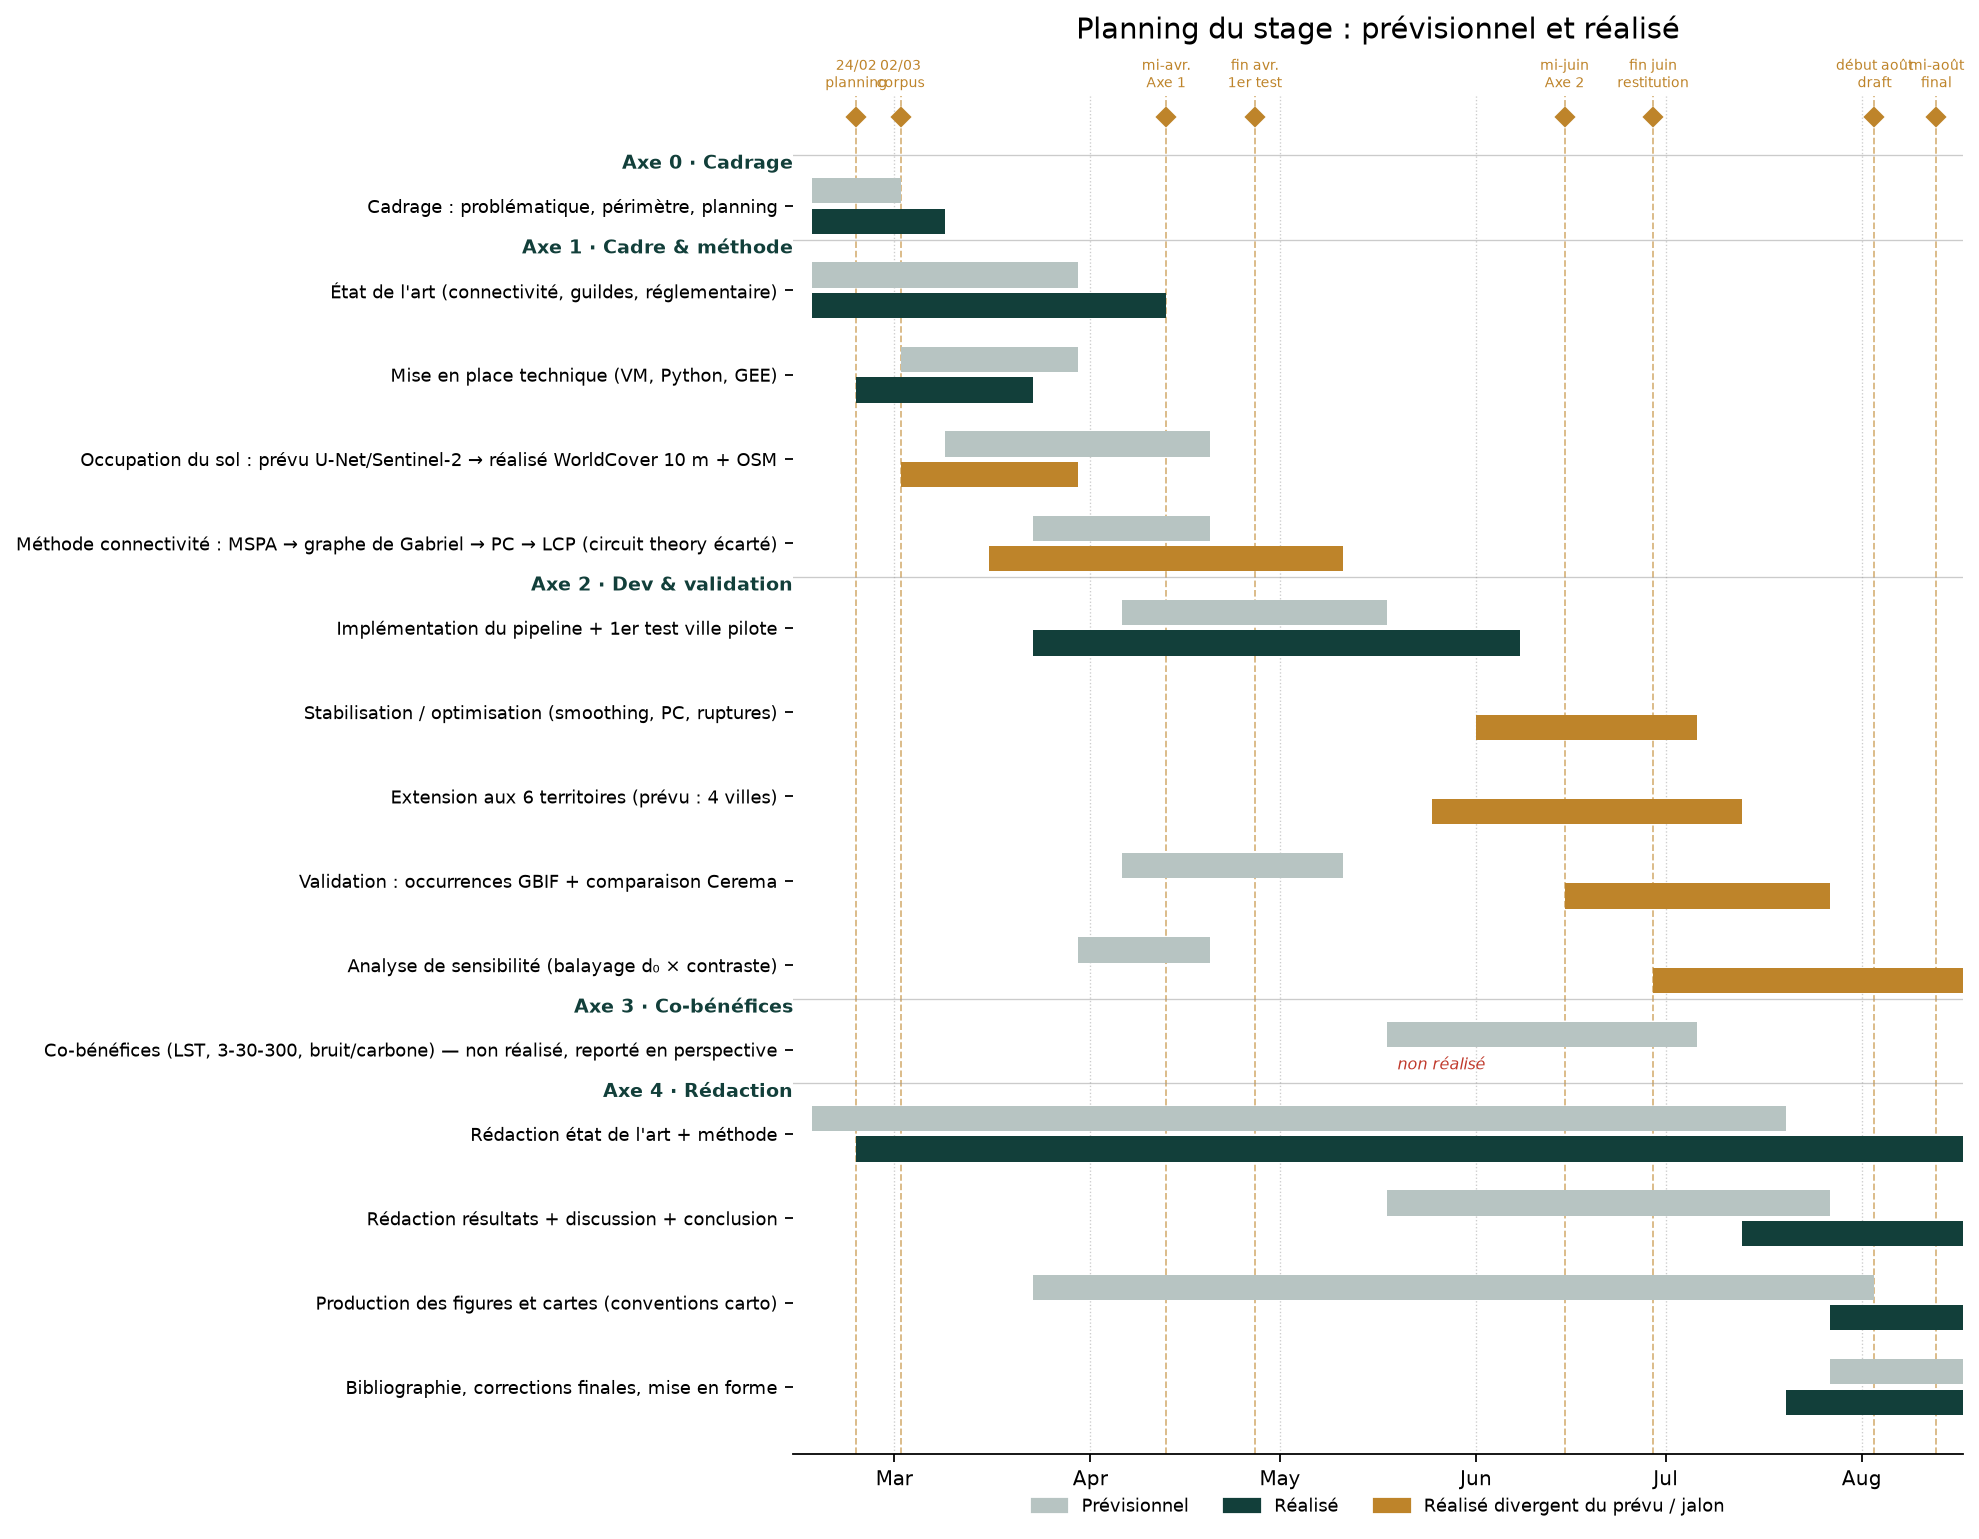
\includegraphics[width=0.98\textwidth]{figures/gantt_stage.png}
\caption{Diagramme de Gantt comparant le planning prévisionnel et le planning réalisé.}
\label{fig:20}
\end{figure}

Le suivi s'est appuyé sur un point hebdomadaire avec mon tuteur, le lundi matin, consacré à l'avancement, aux réorientations et au guidage du travail. À l'échelle de l'entreprise, une réunion mensuelle réunissait les trois pôles (commercial ; ingénierie recherche et projets, mon pôle ; ingénierie visualisation et infrastructure), où je présentais régulièrement l'avancée de mon sujet. L'équipe R\&D tenait aussi une réunion hebdomadaire, le mercredi matin, dédiée à la veille, au partage de données, de méthodes et d'articles, et à la présentation par l'un de ses membres d'un sujet exploré, selon un format structuré (contexte, acquis, pratiques actuelles, perspectives, positionnement de l'équipe) suivi d'un court quiz ; j'y ai présenté la connectivité écologique urbaine.

Le stage s'est aussi inséré dans le consortium du projet UrbiVerde, aux côtés de CS Group et du Cerema. J'ai participé à des réunions techniques réunissant ces partenaires, consacrées à un état des lieux des connaissances et des indicateurs déjà développés par chacun et à leur articulation : il s'agissait de situer l'indicateur de connectivité parmi les briques existantes de la future plateforme et d'éviter les redondances. J'ai également pris part à un groupe de travail sur les trames animé par des experts du Cerema, qui a nourri l'alignement du vocabulaire et de la méthode sur le cadre de la Trame verte et bleue (\hyperref[chap:1]{chapitre 1}). En parallèle, le Cerema a conduit des ateliers avec les villes pilotes pour recueillir leurs besoins et leurs attentes vis-à-vis de la plateforme et dresser l'état de ce qu'elles utilisent déjà : Nancy et La Roche-sur-Yon à distance, Perpignan sur site au Cerema de Toulouse.

Ces retours ont directement infléchi la conception. Le tableau de bord a été simplifié pour rester lisible par des utilisateurs qui ne sont pas écologues : une entrée par territoire et par profil écologique, un vocabulaire accessible et un affichage épuré des couches. Les gestionnaires se sont surtout montrés intéressés par la simulation d'aménagements, pour en chiffrer l'effet sur la connectivité et arbitrer entre projets, et par la sensibilisation aux enjeux qu'elle permet, davantage que par le détail méthodologique. Ce constat a orienté la restitution vers l'usage prospectif de l'outil (\hyperref[sec:3.6]{§3.6}, \hyperref[sec:4.3]{§4.3}) plutôt que vers la seule cartographie de l'état existant.

\section{Choix de méthode : essais et alignement}\label{sec:6.2}

Les choix de méthode se sont arrêtés progressivement en cours de stage, chacun consigné dans le journal de décisions (le decision\_log, registre daté où chaque choix, incident ou test est reporté). L'alignement méthodologique avec le Cerema, conduit à partir de son rapport et lors de discussions avec ses chercheurs (J.-F. Bretaud, V. Rauel, D. Crozier), y a joué un rôle déterminant. Les choix eux-mêmes et leurs justifications techniques sont exposés au \hyperref[chap:2]{chapitre 2} ; je retrace ici la manière dont ils se sont imposés, plutôt que de les ré-argumenter.

Le principe de différenciation a été fixé en premier : partie d'une table de résistance unique, j'y ai renoncé au profit de profils écologiques, seuls porteurs d'une information fonctionnelle plutôt que d'une simple mesure de structure. Restait ensuite à choisir comment différencier : les sous-trames du Cerema supposant une occupation du sol plus fine que WorldCover, j'ai défini les profils par syndrome de déplacement ; et l'occupation du sol a été prise toute faite plutôt que produite sur mesure (\hyperref[chap:2]{chapitre 2}). Le périmètre s'est enfin réduit de cinq à quatre profils au fil de l'alignement des frictions avec le Cerema (détaillé au \hyperref[chap:2]{chapitre 2}).

Deux simplifications ont été assumées faute de temps. La qualité des noyaux, d'abord pensée multicritère, a été ramenée à un critère morphologique, ce que je reprends comme limite au \hyperref[chap:4]{chapitre 4}. Les métriques d'importance par flux (dPC, intermédiarité), qui hiérarchisent les liens selon le flux qu'ils portent et leur position dans le réseau, ont été désactivées : présenter un lien comme moins important qu'un autre, sur la foi d'un classement non validé, pourrait orienter à tort des décisions d'aménagement lourdes ; la restitution vise donc à montrer où agir plutôt qu'à hiérarchiser les liens, mais leur implémentation reste conservée et réactivable.

\section{Débogage et fiabilisation}\label{sec:6.3}

Une part substantielle du travail a porté sur le débogage et la fiabilisation de la chaîne, en particulier sur la construction du graphe. Plusieurs liens apparaissaient à tort coupés ou en échec pour des raisons de traitement, et non écologiques : un index de n\oe{}uds désynchronisé par l'étape de lissage, ou un chemin de moindre coût réduit à un seul pixel. Le lissage des tracés ne joue qu'un rôle d'affichage, mais un défaut à cette étape suffisait à fausser le diagnostic de fonctionnalité.

Au-delà de ces anomalies de traitement, j'ai cherché à savoir jusqu'où la chaîne reste robuste et où elle atteint ses limites. J'ai traité des cas limites, comme une tache d'habitat de très grande taille qui faisait diverger l'étape de lissage des géométries et a nécessité un garde-fou, et j'ai contrôlé la robustesse de la chaîne sur des emprises à faible couverture OpenStreetMap et sur de grandes étendues.

Ces anomalies ont été repérées en comparant systématiquement les sorties aux cartes attendues, en particulier sur Toulouse dont je connais le terrain, puis résolues en combinant plusieurs ressources : l'agent de programmation pour explorer les pistes et réécrire le code, les échanges avec le tuteur pour trancher les cas ambigus, et la documentation des bibliothèques. Chaque correctif a été validé en confrontant les sorties avant et après correction.

\section{Performance et passage à l'échelle}\label{sec:6.4}

Le passage à l'échelle des grandes villes a constitué un enjeu technique en soi : le graphe de Toulouse compte environ 9 400 n\oe{}uds (taches d'habitat et espaces relais), et le calcul de l'indice de connectivité sur toutes leurs paires, de coût quadratique, devient trop lourd pour une implémentation directe. Les étapes les plus coûteuses en calcul ont été identifiées puis optimisées en remplaçant les opérations en cause, comme la comparaison de toutes les paires de n\oe{}uds ou de chaque corridor à la fusion de tous les habitats, par des calculs vectorisés ou accélérés par un index spatial.

Le calcul de l'indice de connectivité, d'abord, passait par une double boucle Python sur toutes les paires de n\oe{}uds ; réécrit avec un plus court chemin matriciel (scipy) et une somme vectorisée (numpy), il gagne un facteur d'environ 29 sur Perpignan (de 28,5 s à 0,98 s) et davantage sur Toulouse (de plus de deux heures à une trentaine de secondes), pour un résultat validé identique à l'original. Le découpage en segments de corridor, ensuite, dominait le temps de calcul sur Toulouse (environ 77 minutes, concentrées dans deux opérations portant sur la fusion de toutes les taches d'habitat en une seule géométrie, longue à intersecter) ; en ne traitant chaque corridor que contre les habitats qu'il intersecte réellement et en préparant la géométrie de test une seule fois, il descend à quelques minutes, pour des sorties géométriquement identiques. Le lissage des n\oe{}uds, enfin, est passé d'une douzaine d'heures à une dizaine de secondes en remplaçant un appel par n\oe{}ud par un unique appel groupé (Tableau 4).

\begin{table}[H]
\centering
\caption{Optimisations des étapes coûteuses (temps avant/après, sur le territoire concerné).}
\begin{tabularx}{\textwidth}{>{\raggedright\arraybackslash}X >{\raggedright\arraybackslash}X >{\raggedright\arraybackslash}X >{\raggedright\arraybackslash}X}
\toprule
\textbf{Étape optimisée} & \textbf{Avant} & \textbf{Après} & \textbf{Levier} \\
\midrule
Indice de connectivité (PC), Toulouse & plus de 2 h & environ 30 s & plus court chemin matriciel (scipy) + somme vectorisée (numpy) \\
Indice de connectivité (PC), Perpignan & 28,5 s & 0,98 s & idem (facteur d'environ 29) \\
Découpage en segments de corridor, Toulouse & environ 77 min & quelques minutes & intersection ciblée + géométrie de test préparée une seule fois \\
Lissage des n\oe{}uds & une douzaine d'heures & une dizaine de secondes & appel groupé unique au lieu d'un appel par n\oe{}ud \\
\bottomrule
\end{tabularx}
\end{table}

Dans les trois cas, les sorties après optimisation ont été validées identiques (indice) ou géométriquement identiques (segments) à celles d'avant.

Ces gains s'appuient sur des bibliothèques générales matures (scikit-image, scipy, geopandas, networkx). Le coût par profil écologique reste ensuite dominé par deux étapes intrinsèquement exigeantes, la construction du graphe et le tracé des moindres coûts.

Le re-run complet donne l'ordre de grandeur du coût par territoire, des plus petites emprises aux plus grandes :

\begin{table}[H]
\centering
\begin{tabularx}{\textwidth}{>{\raggedright\arraybackslash}X >{\raggedright\arraybackslash}X}
\toprule
\textbf{Territoire} & \textbf{Temps total (4 profils écologiques)} \\
\midrule
Kourou & 8 min \\
Perpignan & 17 min \\
Nancy & 23 min \\
La Rochelle & 35 min \\
La Roche-sur-Yon & 116 min \\
Toulouse & 156 min \\
\bottomrule
\end{tabularx}
\end{table}

Le coût se concentre sur les grandes emprises et sur deux étapes : pour le profil écologique le plus lourd (Toulouse, petit mammifère terrestre, 86 minutes), le tracé des moindres coûts (environ 50 minutes) et la construction du graphe de Gabriel (environ 26 minutes) représentent à eux seuls près de neuf dixièmes du temps, toutes les autres étapes (segmentation, indice de connectivité, dispersion, segments) restant de l'ordre de quelques minutes au plus.

L'optimisation m'a appris à profiler avant d'optimiser, le goulot d'étranglement n'étant pas toujours là où on l'imagine, et à privilégier des leviers structurels (vectorisation, index spatial, appel groupé unique) plutôt que des micro-optimisations au jugé.

\section{Environnement de travail et assistance par IA}\label{sec:6.5}

Le développement a été mené dans l'éditeur VSCode connecté à une machine virtuelle distante hébergée chez OVH (350 Go de mémoire vive, 24 c\oe{}urs, GPU Nvidia H100), dimensionnée pour traiter de grandes emprises. J'ai également conduit l'alignement méthodologique avec le Cerema jusqu'à la mise en place d'une comparaison des deux méthodes sur La Rochelle (\hyperref[sec:3.5]{§3.5}, \hyperref[sec:4.4]{§4.4}). Cette collaboration a évolué au cours du stage : le projet a démarré en commun, mais l'indicateur de connectivité a ensuite avancé de mon côté, les contraintes de temps différant, un stage de six mois m'ayant conduite à prendre seule plusieurs décisions méthodologiques. Mon travail est transmis au Cerema, qui s'en servira pour construire une version consolidée destinée à la plateforme, appuyée le cas échéant sur des données françaises et sur le produit Green Urban Sat pour l'occupation du sol, dont la couche différerait alors de celle retenue ici ; une réunion en septembre doit permettre de converger sur une méthode commune. Le travail s'est également inscrit dans la vie de l'équipe R\&D, dont les réunions régulières portaient sur la veille technique, les difficultés rencontrées et la présentation aux autres membres des sujets en cours, appuyée sur des supports et des quiz.

Le code a été produit avec l'assistance d'un agent de programmation (Claude Code), encadré par une convention de travail écrite interne à l'équipe R\&D de Murmuration. Cette convention fonde la fiabilité de la démarche, et mérite d'être décrite pour un lecteur non familier de ces outils. L'assistant y est sceptique par défaut : il lui est demandé de chercher d'abord le point faible d'une idée avant de la valider, et les formules de complaisance lui sont proscrites. Tout énoncé qu'il ne peut pas vérifier doit être signalé comme tel, et chaque affirmation porte un marqueur de confiance. La règle centrale est que sa production n'est jamais auto-validante : l'ingénieur la relit, la teste, la valide et la signe ; le recours à une IA ne dégage en rien de la responsabilité des erreurs d'un livrable. Le code n'est écrit que sur demande explicite ; chaque décision, incident ou test est consigné dans un journal daté ; et aucun résultat n'est déclaré terminé sans passer une série de contrôles systématiques (complétude des sorties, projection et bornes géographiques, plausibilité physique des valeurs). Le temps de développement s'est ainsi déplacé de l'écriture du code vers sa relecture et son contrôle, pour un code souvent mieux optimisé, la responsabilité du résultat restant entière à l'ingénieur.

\section{Organisation, reproductibilité et passation}\label{sec:6.6}

Le travail a été conduit de façon itérative et traçable : une convention de projet, un nettoyage non destructif conservant les essais, le passage à des formats standard (.geojson, .csv) et la tenue continue du journal de décisions. Le fichier de configuration des profils écologiques, qui isole les paramètres métier du code, est un choix de conception délibéré : il permet de modifier un profil sans intervenir sur le reste de la chaîne.

L'objectif est que l'équipe puisse relancer la chaîne sans moi. La passation repose sur trois éléments laissés à l'équipe : le code, versionné dans un dépôt Git ; les paramètres métier, isolés dans le fichier de configuration des profils écologiques et modifiables sans toucher à la chaîne ; et la documentation de suivi (journal de décisions, vue d'ensemble des notebooks, structure et arborescence des données). Deux compléments renforceraient la reprise et restent à produire : un fichier README d'entrée décrivant l'installation et le lancement de bout en bout, et le dossier d'industrialisation prévu par la convention de l'équipe (instantané du code, notebook de lancement, tables des entrées et des transformations), qui rassemblerait en un seul point ce qui est nécessaire au passage en production. [À CONFIRMER : emplacement du dépôt et documentation effectivement laissée à la fin du stage.] Ces deux compléments seront produits lors de l'industrialisation de la chaîne dans UrbiVerde, que l'équipe poursuit.

Ces choix inscrivent la chaîne dans les principes FAIR de gestion des données de recherche \hyperref[sec:bibliographie]{(Wilkinson et al., 2016)} : ses sorties se veulent \textit{trouvables} (arborescence normalisée, nommage systématique, inventaire des sources en \hyperref[annexe:A]{annexe A}), \textit{accessibles} (données d'entrée entièrement ouvertes, code versionné), \textit{interopérables} (formats standard .geojson, .tif et .csv, projection déclarée, nomenclature d'occupation du sol explicite) et \textit{réutilisables} (paramètres métier isolés et documentés, provenance tracée, journal de décisions). Deux dettes limitent toutefois encore la reprise et restent à lever pour l'industrialisation : la chaîne importe certains modules par des chemins relatifs vers d'autres espaces de travail, ce qui la lie à une arborescence précise et l'empêche de tourner telle quelle ailleurs (à corriger en empaquetant proprement ces dépendances) ; et elle dépend d'Earth Engine (authentification, quotas, disponibilité de l'API), dépendance externe à déclarer et à encapsuler.

\section{Apports personnels}\label{sec:6.7}

Sur le plan technique, ce stage m'a permis de consolider la programmation géospatiale en Python (xarray et rioxarray pour le raster, geopandas et shapely pour le vecteur, networkx pour les graphes, scikit-image pour la morphologie mathématique) dans un cas pratique suivi de bout en bout : disposer d'un fil rouge, d'un cas d'étude unique, aide à en comprendre le détail bien plus qu'un exercice isolé. La théorie des graphes appliquée à l'écologie du paysage était nouvelle pour moi : l'écologie m'était familière depuis ma licence, mais je ne l'avais jamais abordée avec une modélisation aussi poussée, et la question de savoir comment traduire ces concepts en calcul m'a particulièrement intéressée. La chaîne d'observation de la Terre (Google Earth Engine, OpenStreetMap), entrevue pendant le master et le projet collectif d'atelier géomatique, a été mise en pratique à plus grande échelle. Enfin, l'optimisation et le passage à l'échelle (profilage, vectorisation, index spatial) étaient nouveaux et constituent un acquis transférable.

Au-delà de la technique, travailler dans une entreprise privée était nouveau pour moi, qui avais jusque-là évolué en laboratoire de recherche. L'attention portée à l'utilité et au rendement s'est révélée stimulante : un travail orienté vers un usage concret avance plus vite et se décide plus facilement, l'objectif final aidant à trancher les choix intermédiaires et à hiérarchiser l'effort.

La principale compétence que j'en retire est la traduction d'un modèle écologique en une chaîne reproductible, puis en couches directement actionnables par des non-spécialistes : faire passer un raisonnement d'écologue à un outil que d'autres peuvent exécuter, comprendre et mobiliser pour décider.

Le travail en consortium et le dialogue avec des utilisateurs non spécialistes constituent une compétence à part entière. J'ai constaté que les détails techniques, sur lesquels portait pourtant l'essentiel de mon travail, n'intéressaient qu'une faible part des interlocuteurs, ce qui oblige à prendre du recul et à traduire son travail dans les termes de l'usage. Gérer un périmètre mouvant m'a appris l'importance de points réguliers pour resserrer et prioriser : le périmètre n'est jamais acquis, il se réajuste en continu. La rigueur et la traçabilité (journal de décisions, convention de travail, contrôles automatisés des sorties) sont devenues une pratique naturelle, d'autant qu'elles sont courantes dans l'équipe.

Avec du recul, ce que je referais différemment est d'entrer plus tôt en contact avec les experts extérieurs et de moins hésiter à solliciter leur expertise, qu'il s'agisse du Cerema ou d'autres bureaux d'études : ces échanges, quand ils ont eu lieu, ont été parmi les plus utiles. La limite que j'assume le plus lucidement, au-delà des limites techniques du \hyperref[chap:4]{chapitre 4}, est d'avoir avancé seule sur l'indicateur, sous la contrainte de six mois, sans la co-construction plus poussée avec le Cerema ni la validation de terrain qu'un temps plus long auraient permises.

Enfin, ce stage a précisé mon projet professionnel. Je poursuis dans l'équipe sur des sujets d'environnement appuyés sur l'observation de la Terre. Il m'a permis d'associer une dimension de recherche, que j'avais appréciée lors d'une précédente expérience en océanographie, à un projet concret dont les résultats sont destinés à être réellement utilisés : là où la recherche peut donner le sentiment de s'adresser surtout à d'autres chercheurs, je trouve ici un travail taillé pour des utilisateurs finaux. Il relie aussi l'écologie et l'environnement aux compétences techniques de la géomatique et de la télédétection, dans la continuité de mon parcours.

\chapter*{Bibliographie}
\addcontentsline{toc}{chapter}{Bibliographie}
\phantomsection\label{sec:bibliographie}

Adriaensen, F., Chardon, J. P., De Blust, G., Swinnen, E., Villalba, S., Gulinck, H., \& Matthysen, E. (2003). The application of 'least-cost' modelling as a functional landscape model. \textit{Landscape and Urban Planning}, 64(4), 233--247. \url{https://doi.org/10.1016/s0169-2046(02})00242-6

Albert, C. H., \& Chaurant, J. (2018). Comment choisir les espèces pour identifier des réseaux écologiques cohérents entre les niveaux administratifs et les niveaux biologiques ? \textit{Sciences Eaux \& Territoires}, 25, 6 p.

Andelman, S. J., \& Fagan, W. F. (2000). Umbrellas and flagships: efficient conservation surrogates or expensive mistakes? \textit{PNAS}, 97(11), 5954--5959. \url{https://doi.org/10.1073/pnas.100126797}

Aronson, M. F. J., La Sorte, F. A., Nilon, C. H., Katti, M., Goddard, M. A., Lepczyk, C. A., Warren, P. S., Williams, N. S. G., Cilliers, S., Clarkson, B., Dobbs, C., Dolan, R., Hedblom, M., Klotz, S., Kooijmans, J. L., Kühn, I., MacGregor-Fors, I., McDonnell, M., Mörtberg, U., \ldots{} Winter, M. (2014). A global analysis of the impacts of urbanization on bird and plant diversity reveals key anthropogenic drivers. \textit{Proceedings of the Royal Society B}, 281, 20133330. \url{https://doi.org/10.1098/rspb.2013.3330} et 25 \% (plantes) du non-urbain ; les villes restent majoritairement natives)

Avon, C., Bergès, L., \& Roche, P. (2014). Comment analyser la connectivité écologique des trames vertes ? Cas d'étude en région méditerranéenne. \textit{Sciences Eaux \& Territoires}, 14, 14--19. \url{https://doi.org/10.14758/SET-REVUE.2014.14.03}

Balbi, M. (2017). \textit{Validation de la fonctionnalité des continuités écologiques en milieu urbain : approches plurispécifiques et multi-sites} (thèse de doctorat, 181 p.). \url{https://doi.org/10.70675/7654ce21z633fz487az8505z03f17e949659}

Balbi, M., Petit, E. J., Croci, S., Nabucet, J., Georges, R., Madec, L., \& Ernoult, A. (2019). Ecological relevance of least cost path analysis: An easy implementation method for landscape urban planning. \textit{Journal of Environmental Management}, 244, 61--68. \url{https://doi.org/10.1016/j.jenvman.2019.04.124}

Balbi, M., Croci, S., Petit, E. J., Butet, A., Georges, R., Madec, L., Caudal, J.-P., \& Ernoult, A. (2021). Least-cost path analysis for urban greenways planning: a test with moths and birds across two habitats and two cities. \textit{Journal of Applied Ecology}, 58(3), 632--643. \url{https://doi.org/10.1111/1365-2664.13800}

Barrington-Leigh, C., \& Millard-Ball, A. (2017). The world's user-generated road map is more than 80\% complete. \textit{PLOS ONE}, 12(8), e0180698. \url{https://doi.org/10.1371/journal.pone.0180698}

Barthel, L. M. F., Wehner, D., Schmidt, A., Berger, A., Hofer, H., \& Fickel, J. (2020). Unexpected gene-flow in urban environments: the example of the European hedgehog. \textit{Animals}, 10(12), 2315. \url{https://doi.org/10.3390/ani10122315}

Beger, M., Metaxas, A., Balbar, A. C., McGowan, J. A., Daigle, R., Kuempel, C. D., Treml, E. A., \& Possingham, H. P. (2022). Demystifying ecological connectivity for actionable spatial conservation planning. \textit{Trends in Ecology \& Evolution}, 37(12), 1079--1091. \url{https://doi.org/10.1016/j.tree.2022.09.002}

Beier, P., Majka, D. R., \& Spencer, W. D. (2008). Forks in the road: choices in procedures for designing wildland linkages. \textit{Conservation Biology}, 22(4), 836--851. \url{https://doi.org/10.1111/j.1523-1739.2008.00942.x}

Bélisle, M., Desrochers, A., \& Fortin, M.-J. (2001). Influence of forest cover on the movements of forest birds: a homing experiment. \textit{Ecology}, 82(7), 1893--1904. \url{https://doi.org/10.1890/0012-9658(2001})082[1893:iofcot]2.0.co;2

Beninde, J., Veith, M., \& Hochkirch, A. (2015). Biodiversity in cities needs space: a meta-analysis of factors determining intra-urban biodiversity variation. \textit{Ecology Letters}, 18(6), 581--592. \url{https://doi.org/10.1111/ele.12427}

Beninde, J., Feldmeier, S., Werner, M., Peroverde, D., Schulte, U., Hochkirch, A., \& Veith, M. (2016). Cityscape genetics: structural versus functional connectivity of an urban lizard population. \textit{Molecular Ecology}, 25(20), 4984--5000. \url{https://doi.org/10.1111/mec.13810}

Blaschke, T. (2010). Object based image analysis for remote sensing. \textit{ISPRS Journal of Photogrammetry and Remote Sensing}, 65(1), 2--16. \url{https://doi.org/10.1016/j.isprsjprs.2009.06.004}

Boakes, E. H., McGowan, P. J. K., Fuller, R. A., Chang-qing, D., Clark, N. E., O'Connor, K., \& Mace, G. M. (2010). Distorted views of biodiversity: spatial and temporal bias in species occurrence data. \textit{PLoS Biology}, 8(6), e1000385. \url{https://doi.org/10.1371/journal.pbio.1000385}

Borghi, C., Francini, S., Chiesi, L., Mancuso, S., Tupikina, L., Caldarelli, G., Moi, J., Vangi, E., D'Amico, G., De Luca, G., \& Chirici, G. (2026). \textit{Integrating Earth Observation and Graph Theory to Evaluate Urban Green Spaces Connectivity Across European Capitals} [preprint]. bioRxiv. \url{https://doi.org/10.64898/2026.01.29.702234}

Bowman, J., Adey, E., Angoh, S. Y. J., Baici, J. E., Brown, M. G. C., Cordes, C., Dupuis, A. E., Newar, S. L., Scott, L. M., \& Solmundson, K. (2020). Effects of cost surface uncertainty on current density estimates from circuit theory. \textit{PeerJ}, 8, e9617. \url{https://doi.org/10.7717/peerj.9617}

Braaker, S., Ghazoul, J., Obrist, M. K., \& Moretti, M. (2014). Habitat connectivity shapes urban arthropod communities: the key role of green roofs. \textit{Ecology}, 95(4), 1010--1021. \url{https://doi.org/10.1890/13-0705.1}

Braaker, S., Kormann, U. G., Bontadina, F., \& Obrist, M. K. (2017). Prediction of genetic connectivity in urban ecosystems by combining detailed movement data, genetic data and multi-path modelling. \textit{Landscape and Urban Planning}, 160, 107--114. \url{https://doi.org/10.1016/j.landurbplan.2016.12.011}

Brown, C. F., Brumby, S. P., Guzder-Williams, B., Birch, T., Hyde, S. B., Mazzariello, J., Czerwinski, W., Pasquarella, V. J., Haertel, R., Ilyushchenko, S., Schwehr, K., Weisse, M., Stolle, F., Hanson, C., Guinan, O., Moore, R., \& Tait, A. M. (2022). Dynamic World, near real-time global 10 m land use land cover mapping. \textit{Scientific Data}, 9, 251. \url{https://doi.org/10.1038/s41597-022-01307-4}

Casalegno, S., Anderson, K., Cox, D. T. C., Hancock, S., \& Gaston, K. J. (2017). Ecological connectivity in the three-dimensional urban green volume using waveform airborne lidar. \textit{Scientific Reports}, 7, 45571. \url{https://doi.org/10.1038/srep45571}

Cerema, direction territoriale Sud-Ouest (2025). \textit{Identification des continuités écologiques urbaines : Communauté d'agglomération de La Rochelle} (rapport rédigé par F. Jamin \& V. Rauel, 20 juin 2025). CeremaDoc.

Code de l'environnement, article L. 371-3 (Trame verte et bleue : prise en compte par les documents d'urbanisme). Légifrance.

Commission européenne (2020). \textit{Stratégie de l'UE en faveur de la biodiversité à l'horizon 2030}. COM(2020) 380 final.

Cushman, S. A. (2006). Effects of habitat loss and fragmentation on amphibians: a review and prospectus. \textit{Biological Conservation}, 128(2), 231--240. \url{https://doi.org/10.1016/j.biocon.2005.09.031}

Cushman, S. A., McKelvey, K. S., Hayden, J., \& Schwartz, M. K. (2006). Gene flow in complex landscapes: testing multiple hypotheses with causal modeling. \textit{The American Naturalist}, 168(4), 486--499. \url{https://doi.org/10.1086/506976}

Damschen, E. I., Brudvig, L. A., Burt, M. A., Fletcher, R. J., Haddad, N. M., Levey, D. J., Orrock, J. L., Resasco, J., \& Tewksbury, J. J. (2019). Ongoing accumulation of plant diversity through habitat connectivity in an 18-year experiment. \textit{Science}, 365(6460), 1478--1480. \url{https://doi.org/10.1126/science.aax8992}

Delaney, K. S., Riley, S. P. D., \& Fisher, R. N. (2010). A rapid, strong, and convergent genetic response to urban habitat fragmentation in four divergent and widespread vertebrates. \textit{PLoS ONE}, 5(9), e12767. \url{https://doi.org/10.1371/journal.pone.0012767}

Deslauriers, M. R., Asgary, A., Nazarnia, N., \& Jaeger, J. A. G. (2018). Implementing the connectivity of natural areas in cities as an indicator in the City Biodiversity Index (CBI). \textit{Ecological Indicators}, 94, 99--113. \url{https://doi.org/10.1016/j.ecolind.2017.02.028}

Diniz, M. F., Cushman, S. A., Machado, R. B., \& De Marco Júnior, P. (2020). Landscape connectivity modeling from the perspective of animal dispersal. \textit{Landscape Ecology}, 35(1), 41--58. \url{https://doi.org/10.1007/s10980-019-00935-3}

Dutta, T., De Barba, M., Selva, N., Fedorca, A. C., Maiorano, L., Thuiller, W., Zedrosser, A., Signer, J., Pflüger, F., Frank, S., Lucas, P. M., \& Balkenhol, N. (2023). An objective approach to select surrogate species for connectivity conservation. \textit{Frontiers in Ecology and Evolution}, 11, 1078649. \url{https://doi.org/10.3389/fevo.2023.1078649}

El-Gabbas, A. (2026). A global, taxon-stratified, high-resolution sampling-effort dataset from GBIF for bias-aware ecological modelling. \textit{Diversity and Distributions} (early view). \url{https://doi.org/10.1111/ddi.70205}

Elmqvist, T., Setälä, H., Handel, S., van der Ploeg, S., Aronson, J., Blignaut, J., Gómez-Baggethun, E., Nowak, D., Kronenberg, J., \& de Groot, R. (2015). Benefits of restoring ecosystem services in urban areas. \textit{Current Opinion in Environmental Sustainability}, 14, 101--108. \url{https://doi.org/10.1016/j.cosust.2015.05.001}

ESA WorldCover consortium (2021). \textit{ESA WorldCover Product User Manual v1.0}. VITO / ESA WorldCover project.

Estrada, E., \& Bodin, Ö. (2008). Using network centrality measures to manage landscape connectivity. \textit{Ecological Applications}, 18(7), 1810--1825. \url{https://doi.org/10.1890/07-1419.1,} pour hiérarchiser les taches et les liens selon le flux qu'ils portent dans le réseau, §1.5.1)

Etherington, T. R. (2016). Least-cost modelling and landscape ecology: concepts, applications, and opportunities. \textit{Current Landscape Ecology Reports}, 1(1), 40--53. \url{https://doi.org/10.1007/s40823-016-0006-9}

Fahrig, L., Pedlar, J. H., Pope, S. E., Taylor, P. D., \& Wegner, J. F. (1995). Effect of road traffic on amphibian density. \textit{Biological Conservation}, 73(3), 177--182. \url{https://doi.org/10.1016/0006-3207(94})00102-v

Fahrig, L. (2003). Effects of habitat fragmentation on biodiversity. \textit{Annual Review of Ecology, Evolution, and Systematics}, 34, 487--515. \url{https://doi.org/10.1146/annurev.ecolsys.34.011802.132419}

Fahrig, L. (2013). Rethinking patch size and isolation effects: the habitat amount hypothesis. \textit{Journal of Biogeography}, 40(9), 1649--1663. \url{https://doi.org/10.1111/jbi.12130}

Fall, A., Fortin, M.-J., Manseau, M., \& O'Brien, D. (2007). Spatial graphs: principles and applications for habitat connectivity. \textit{Ecosystems}, 10(3), 448--461. \url{https://doi.org/10.1007/s10021-007-9038-7}

Foltête, J.-C., Clauzel, C., \& Vuidel, G. (2012). A software tool dedicated to the modelling of landscape networks (Graphab). \textit{Environmental Modelling \& Software}, 38, 316--327. \url{https://doi.org/10.1016/j.envsoft.2012.07.002} calibré par un couple distance/probabilité)

Francis, C. D., \& Barber, J. R. (2013). A framework for understanding noise impacts on wildlife. \textit{Biological Conservation}, 166, 7--15. \url{https://doi.org/10.1890/120183}

Gabriel, K. R., \& Sokal, R. R. (1969). A new statistical approach to geographic variation analysis. \textit{Systematic Zoology}, 18(3), 259--278. \url{https://doi.org/10.2307/2412323}

Galpern, P., Manseau, M., \& Fall, A. (2011). Patch-based graphs of landscape connectivity: a guide to construction, analysis and application for conservation. \textit{Biological Conservation}, 144(1), 44--55. \url{https://doi.org/10.1016/j.biocon.2010.09.002}

Gaston, K. J., Bennie, J., Davies, T. W., \& Hopkins, J. (2013). The ecological impacts of nighttime light pollution: a mechanistic appraisal. \textit{Biological Reviews}, 88(4), 912--927. \url{https://doi.org/10.1111/brv.12036}

Gelmi-Candusso, T. A., Chin, A. T. M., Ruppert, J. L. W., \& Fortin, M.-J. (2025). Urban planning for wildlife connectivity: a multispecies assessment of urban sprawl and SLOSS renaturalization strategies. \textit{Journal of Applied Ecology}, 62, 1007--1023. \url{https://doi.org/10.1111/1365-2664.70007}

Gilbert-Norton, L., Wilson, R., Stevens, J. R., \& Beard, K. H. (2010). A meta-analytic review of corridor effectiveness. \textit{Conservation Biology}, 24(3), 660--668. \url{https://doi.org/10.1111/j.1523-1739.2010.01450.x}

Goicolea, T., et al. (2021). Randomized shortest paths for connectivity modelling. \textit{Movement Ecology}, 9, 52. [titre exact à confirmer]

Grafius, D. R., Corstanje, R., Siriwardena, G. M., Plummer, K. E., \& Harris, J. A. (2017). A bird's eye view: using circuit theory to study urban landscape connectivity for birds. \textit{Landscape Ecology}, 32(9), 1771--1787. \url{https://doi.org/10.1007/s10980-017-0548-1}

Grimm, N. B., Faeth, S. H., Golubiewski, N. E., Redman, C. L., Wu, J., Bai, X., \& Briggs, J. M. (2008). Global change and the ecology of cities. \textit{Science}, 319(5864), 756--760. \url{https://doi.org/10.1126/science.1150195}

Habrich, A. K., \& Fahrig, L. (2025). Systematic map of urban connectivity research reveals a dearth of validation of connectivity estimates. \textit{Current Landscape Ecology Reports}, 10(1), 5. \url{https://doi.org/10.1007/s40823-025-00106-y}

Haddad, N. M., Brudvig, L. A., Clobert, J., Davies, K. F., Gonzalez, A., Holt, R. D., Lovejoy, T. E., Sexton, J. O., Austin, M. P., Collins, C. D., Cook, W. M., Damschen, E. I., Ewers, R. M., Foster, B. L., Jenkins, C. N., King, A. J., Laurance, W. F., Levey, D. J., Margules, C. R., Melbourne, B. A., Nicholls, A. O., Orrock, J. L., Song, D.-X., \& Townshend, J. R. (2015). Habitat fragmentation and its lasting impact on Earth's ecosystems. \textit{Science Advances}, 1(2), e1500052. \url{https://doi.org/10.1126/sciadv.1500052}

Hale, J. D., Fairbrass, A. J., Matthews, T. J., \& Sadler, J. P. (2012). Habitat composition and connectivity predicts bat presence and activity at foraging sites in a large UK conurbation. \textit{PLoS ONE}, 7(3), e33300. \url{https://doi.org/10.1371/journal.pone.0033300}

Hamer, A. J., \& McDonnell, M. J. (2008). Amphibian ecology and conservation in the urbanising world: a review. \textit{Biological Conservation}, 141(10), 2432--2449. \url{https://doi.org/10.1016/j.biocon.2008.07.020}

Hanski, I. (1994). A practical model of metapopulation dynamics. \textit{Journal of Animal Ecology}, 63(1), 151--162. \url{https://doi.org/10.2307/5591}

Hanski, I. (2011). Habitat loss, the dynamics of biodiversity, and a perspective on conservation. \textit{Ambio}, 40(3), 248--255. \url{https://doi.org/10.1007/s13280-011-0147-3}

Hels, T., \& Buchwald, E. (2001). The effect of road kills on amphibian populations. \textit{Biological Conservation}, 99(3), 331--340. \url{https://doi.org/10.1016/s0006-3207(00})00215-9

Huijser, M. P., \& Bergers, P. J. M. (2000). The effect of roads and traffic on hedgehog (\textit{Erinaceus europaeus}) populations. \textit{Biological Conservation}, 95(1), 111--116. \url{https://doi.org/10.1016/S0006-3207(00})00006-9

Inglada, J., Vincent, A., Arias, M., Tardy, B., Morin, D., \& Rodes, I. (2017). Operational high resolution land cover map production at the country scale using satellite image time series. \textit{Remote Sensing}, 9(1), 95. \url{https://doi.org/10.3390/rs9010095}

Isaac, N. J. B., van Strien, A. J., August, T. A., de Zeeuw, M. P., \& Roy, D. B. (2014). Statistics for citizen science: extracting signals of change from noisy ecological data. \textit{Methods in Ecology and Evolution}, 5(10), 1052--1060. \url{https://doi.org/10.1111/2041-210x.12254}

Ives, C. D., Lentini, P. E., Threlfall, C. G., Ikin, K., Shanahan, D. F., Garrard, G. E., Bekessy, S. A., Fuller, R. A., Mumaw, L., Rayner, L., Rowe, R., Valentine, L. E., \& Kendal, D. (2016). Cities are hotspots for threatened species. \textit{Global Ecology and Biogeography}, 25, 117--126. \url{https://doi.org/10.1111/geb.12404}

Jaeger, J. A. G. (2000). Landscape division, splitting index, and effective mesh size: new measures of landscape fragmentation. \textit{Landscape Ecology}, 15(2), 115--130. \url{https://doi.org/10.1023/a:1008129329289}

Johnson, D. H. (1980). The comparison of usage and availability measurements for evaluating resource preference. \textit{Ecology}, 61(1), 65--71. \url{https://doi.org/10.2307/1937156}

Keeley, A. T. H., Beier, P., Keeley, B. W., \& Fagan, M. E. (2017). Habitat suitability is a poor proxy for landscape connectivity during dispersal and mating movements. \textit{Landscape and Urban Planning}, 161, 90--102. \url{https://doi.org/10.1016/j.landurbplan.2017.01.007}

Keeley, A. T. H., Beier, P., Creech, T., Jones, K., Jongman, R. H., Stonecipher, G., \& Tabor, G. M. (2019). Thirty years of connectivity conservation planning: an assessment of factors influencing plan implementation. \textit{Environmental Research Letters}, 14(10), 103001. \url{https://doi.org/10.1088/1748-9326/ab3234}

Kirk, H., Soanes, K., Amati, M., Bekessy, S., Harrison, L., Parris, K., Ramalho, C., van der Ree, R., \& Threlfall, C. (2023). Ecological connectivity as a planning tool for the conservation of wildlife in cities. \textit{MethodsX}, 10, 101989. \url{https://doi.org/10.1016/j.mex.2022.101989}

Koen, E. L., Garroway, C. J., Wilson, P. J., \& Bowman, J. (2010). The effect of map boundary on estimates of landscape resistance to animal movement. \textit{PLOS ONE}, 5(7), e11785. \url{https://doi.org/10.1371/journal.pone.0011785}

Koen, E. L., Bowman, J., Sadowski, C., \& Walpole, A. A. (2014). Landscape connectivity for wildlife: development and validation of multispecies linkage maps. \textit{Methods in Ecology and Evolution}, 5(7), 626--633. \url{https://doi.org/10.1111/2041-210x.12197}

Konijnendijk, C. C. (2023). Evidence-based guidelines for greener, healthier, more resilient neighbourhoods: introducing the 3-30-300 rule. \textit{Urban Forestry \& Urban Greening}, 70, 127549. \url{https://doi.org/10.1007/s11676-022-01523-z}

Laliberté, J., \& St-Laurent, M.-H. (2020). Validation of functional connectivity modeling: the Achilles' heel of landscape connectivity mapping. \textit{Landscape and Urban Planning}, 202, 103878. \url{https://doi.org/10.1016/j.landurbplan.2020.103878}

Lambeck, R. J. (1997). Focal species: a multi-species umbrella for nature conservation. \textit{Conservation Biology}, 11(4), 849--856. \url{https://doi.org/10.1046/j.1523-1739.1997.96319.x}

LaPoint, S., Balkenhol, N., Hale, J., Sadler, J., \& van der Ree, R. (2015). Ecological connectivity research in urban areas. \textit{Functional Ecology}, 29(7), 868--878. \url{https://doi.org/10.1111/1365-2435.12489}

Larson, R. N., \& Sander, H. A. (2024). Variation in species-specific responses to habitat fragmentation and land cover structure in urban small mammal communities. \textit{Journal of Mammalogy}, 105, gyae121. \url{https://doi.org/10.1093/jmammal/gyae121}

Lechner, A. M., Sprod, D., Carter, O., \& Lefroy, E. C. (2017). Characterising landscape connectivity for conservation planning using a dispersal guild approach. \textit{Landscape Ecology}, 32(1), 99--113. \url{https://doi.org/10.1007/s10980-016-0431-5}

Legendre, P. (1993). Spatial autocorrelation: trouble or new paradigm? \textit{Ecology}, 74(6), 1659--1673. \url{https://doi.org/10.2307/1939924}

Lin, Y., An, W., Gan, M., Shahtahmassebi, A., Ye, Z., Huang, L., Zhu, C., Huang, L., Zhang, J., \& Wang, K. (2021). Spatial grain effects of urban green space cover maps on assessing habitat fragmentation and connectivity. \textit{Land}, 10(10), 1065. \url{https://doi.org/10.3390/land10101065}

Liu, Y., Huang, T.-T., \& Zheng, X. (2022). A method of linking functional and structural connectivity analysis in urban green infrastructure network construction. \textit{Urban Ecosystems}, 25(3), 909--925. \url{https://doi.org/10.1007/s11252-022-01201-2}

Loi n° 2009-967 du 3 août 2009 de programmation relative à la mise en \oe{}uvre du Grenelle de l'environnement (Grenelle I). Journal officiel de la République française, 5 août 2009. Légifrance.

Loi n° 2010-788 du 12 juillet 2010 portant engagement national pour l'environnement (Grenelle II). Journal officiel de la République française, 13 juillet 2010. Légifrance.

Losada-Iglesias, R., García, A. M., Díaz-Varela, E. R., \& Miranda, D. (2024). Proposed spatial decision support system for delineating ecological corridors in green infrastructure planning constrained by lack of data: a case study in Galicia, Spain. \textit{Landscape and Ecological Engineering}. \url{https://doi.org/10.1007/s11355-024-00598-6}

Loss, S. R., Will, T., \& Marra, P. P. (2013). The impact of free-ranging domestic cats on wildlife of the United States. \textit{Nature Communications}, 4, 1396. \url{https://doi.org/10.1038/ncomms2380}

MacArthur, R. H., \& Wilson, E. O. (1967). \textit{The Theory of Island Biogeography}. Princeton University Press.

Macdonald, D. W., \& Barrett, P. (2005). \textit{Guide complet des mammifères de France et d'Europe} (204 p.). Delachaux et Niestlé.

Manly, B. F. J., McDonald, L. L., Thomas, D. L., McDonald, T. L., \& Erickson, W. P. (2002). \textit{Resource Selection by Animals: Statistical Design and Analysis for Field Studies} (2e éd.). Kluwer Academic Publishers.

McRae, B. H., \& Beier, P. (2007). Circuit theory predicts gene flow in plant and animal populations. \textit{PNAS}, 104(50), 19885--19890. \url{https://doi.org/10.1073/pnas.0706568104}

McRae, B. H., Dickson, B. G., Keitt, T. H., \& Shah, V. B. (2008). Using circuit theory to model connectivity in ecology, evolution, and conservation. \textit{Ecology}, 89(10), 2712--2724. \url{https://doi.org/10.1890/07-1861.1}

Melis, R., Malavasi, M., Bazzichetto, M., Caria, M. C., Rivieccio, G., Denaro, A., \& Rocchini, D. (2025). Unravelling bias: a Sardinian perspective on taxonomic, spatial, and temporal biases in vascular plant biodiversity data from GBIF. \textit{Ecological Informatics}, 90, 103289. \url{https://doi.org/10.1016/j.ecoinf.2025.103289}

Meurant, M., Gonzalez, A., Doxa, A., \& Albert, C. H. (2018). Selecting surrogate species for connectivity conservation. \textit{Biological Conservation}, 227, 326--334. \url{https://doi.org/10.1016/j.biocon.2018.09.028}

Mimet, A., Kerbiriou, C., Simon, L., Julien, J.-F., \& Raymond, R. (2020). Contribution of private gardens to habitat availability, connectivity and conservation of the common pipistrelle in Paris. \textit{Landscape and Urban Planning}, 193, 103671. \url{https://doi.org/10.1016/j.landurbplan.2019.103671} fournissent jusqu'à \textasciitilde{}48 \% de la disponibilité d'habitat pour la pipistrelle commune à Paris)

Minor, E. S., \& Urban, D. L. (2008). A graph-theory framework for evaluating landscape connectivity and conservation planning. \textit{Conservation Biology}, 22(2), 297--307. \url{https://doi.org/10.1111/j.1523-1739.2007.00871.x}

Morris, P. A. (1988). A study of home range and movements in the hedgehog (\textit{Erinaceus europaeus}). \textit{Journal of Zoology}, 214(3), 433--449. \url{https://doi.org/10.1111/j.1469-7998.1988.tb03751.x,} \textasciitilde{}12 ha (femelles), et déplacements nocturnes \textasciitilde{}1,6 km/nuit (mâles), max \textasciitilde{}3,14 km)

Niemelä, J., Saarela, S.-R., Söderman, T., Kopperoinen, L., Yli-Pelkonen, V., Väre, S., \& Kotze, D. J. (2010). Using the ecosystem services approach for better planning and conservation of urban green spaces. \textit{Biodiversity and Conservation}, 19(11), 3225--3243. \url{https://doi.org/10.1007/s10531-010-9888-8}

Office français de la biodiversité (OFB). \textit{MOOC Trame verte et bleue} [ressource e-learning]. \url{https://elearning.ofb.fr/course/view.php?id=56} (suivi en début de stage pour l'appropriation du cadre réglementaire et des enjeux de continuité écologique ; formation, non citée comme référence dans le corps).

Ossola, A., Locke, D., Lin, B., \& Minor, E. (2019). Yards increase forest connectivity in urban landscapes. \textit{Landscape Ecology}, 34(12), 2935--2948. \url{https://doi.org/10.1007/s10980-019-00923-7}

Ostapowicz, K., Vogt, P., Riitters, K. H., Kozak, J., \& Estreguil, C. (2008). Impact of scale on morphological spatial pattern of forest. \textit{Landscape Ecology}, 23(9), 1107--1117. \url{https://doi.org/10.1007/s10980-008-9271-2}

Panzacchi, M., Van Moorter, B., Strand, O., Saerens, M., Kivimäki, I., St. Clair, C. C., Herfindal, I., \& Boitani, L. (2016). Predicting the continuum between corridors and barriers to animal movements using step selection functions and randomized shortest paths. \textit{Journal of Animal Ecology}, 85(1), 32--42. \url{https://doi.org/10.1111/1365-2656.12386}

Pascual-Hortal, L., \& Saura, S. (2006). Comparison and development of new graph-based landscape connectivity indices: towards the prioritization of habitat patches and corridors for conservation. \textit{Landscape Ecology}, 21(7), 959--967. \url{https://doi.org/10.1007/s10980-006-0013-z}

Pechanec, V., et al. (2025). Comparaison de méthodes d'évaluation de la connectivité écologique. \textit{Science of the Total Environment}, 180729. [titre exact à confirmer]

Petrenko, J. A., Martin, P. R., Fanelli, R. E., \& Bonier, F. (2024). Urban tolerance does not protect against population decline in North American birds. \textit{Biology Letters}, 20, 20230507. \url{https://doi.org/10.1098/rsbl.2023.0507}

Pinto, N., \& Keitt, T. H. (2009). Beyond the least-cost path: evaluating corridor redundancy using a graph-theoretic approach. \textit{Landscape Ecology}, 24(2), 253--266. \url{https://doi.org/10.1007/s10980-008-9303-y}

Poor, E. E., Jakes, A., Loucks, C., \& Suitor, M. (2014). Modeling fence location and density at a regional scale for use in wildlife management. \textit{PLOS ONE}, 9(1), e83912. \url{https://doi.org/10.1371/journal.pone.0083912}

Pottier, G. (2016). \textit{Les reptiles des Pyrénées}. MNHN, Paris, 352 p. [source : fiche espèce Cerema]

Prima, M.-C., et al. (2024). A comprehensive framework to assess multi-species landscape connectivity. \textit{Methods in Ecology and Evolution}, 15(11). \url{https://doi.org/10.1111/2041-210x.14444}

Pundsack, M., Merkens, L., Weisser, W. W., \& Mimet, A. (2025). A Copernicus pipeline to create a high-resolution land cover map for urban ecological connectivity. [journal à confirmer]

Quiblier (Fédération des Parcs naturels régionaux de France) (2007). \textit{Les éléments de la recherche scientifique mobilisables pour la mise en \oe{}uvre des corridors écologiques}.

Radoux, J., Chomé, G., Jacques, D. C., Waldner, F., Bellemans, N., Matton, N., Lamarche, C., d'Andrimont, R., \& Defourny, P. (2016). Sentinel-2's potential for sub-pixel landscape feature detection. \textit{Remote Sensing}, 8(6), 488. \url{https://doi.org/10.3390/rs8060488}

Rayfield, B., Fortin, M.-J., \& Fall, A. (2010). The sensitivity of least-cost habitat graphs to relative cost surface values. \textit{Landscape Ecology}, 25(4), 519--532. \url{https://doi.org/10.1007/s10980-009-9436-7}

Rayfield, B., Fortin, M.-J., \& Fall, A. (2011). Connectivity for conservation: a framework to classify network measures. \textit{Ecology}, 92(4), 847--858. \url{https://doi.org/10.1890/09-2190.1}

Règlement (UE) 2024/1991 du Parlement européen et du Conseil du 24 juin 2024 relatif à la restauration de la nature. Journal officiel de l'Union européenne, 29 juillet 2024. EUR-Lex.

Rezvani, A., Hemami, M.-R., Goheen, J. R., Kaczensky, P., Pourmanafi, S., Fakheran, S., \& Esmaeili, S. (2024). Rethinking connectivity modeling for high-mobility ungulates: insights from a globally endangered equid. \textit{Landscape Ecology}, 39(4), 73. \url{https://doi.org/10.1007/s10980-024-01873-5}

Ricketts, T. H. (2001). The matrix matters: effective isolation in fragmented landscapes. \textit{The American Naturalist}, 158(1), 87--99. \url{https://doi.org/10.2307/3078900}

Roberge, J.-M., \& Angelstam, P. (2004). Usefulness of the umbrella species concept as a conservation tool. \textit{Conservation Biology}, 18(1), 76--85. \url{https://doi.org/10.1111/j.1523-1739.2004.00450.x}

Robertson, O. J., \& Radford, J. Q. (2009). Gap-crossing decisions of forest birds in a fragmented landscape. \textit{Austral Ecology}, 34(4), 435--446. \url{https://doi.org/10.1111/j.1442-9993.2009.01945.x}

Saura, S., \& Pascual-Hortal, L. (2007). A new habitat availability index to integrate connectivity in landscape conservation planning: comparison with existing indices and application to a case study. \textit{Landscape and Urban Planning}, 83(2--3), 91--103. \url{https://doi.org/10.1016/j.landurbplan.2007.03.005}

Saura, S., \& Torné, J. (2009). Conefor Sensinode 2.2: a software package for quantifying the importance of habitat patches for landscape connectivity. \textit{Environmental Modelling \& Software}, 24(1), 135--139. \url{https://doi.org/10.1016/j.envsoft.2008.05.005}

Saura, S., \& Rubio, L. (2010). A common currency for the different ways in which patches and links can contribute to habitat availability and connectivity in the landscape. \textit{Ecography}, 33(3), 523--537. \url{https://doi.org/10.1111/j.1600-0587.2009.05760.x}

Saura, S., Estreguil, C., Mouton, C., \& Rodríguez-Freire, M. (2011). Network analysis to assess landscape connectivity trends: application to European forests (1990--2000). \textit{Ecological Indicators}, 11(2), 407--416. \url{https://doi.org/10.1016/j.ecolind.2010.06.011}

Saura, S., Bodin, Ö., \& Fortin, M.-J. (2014). Stepping stones are crucial for species' long-distance dispersal and range expansion through habitat networks. \textit{Journal of Applied Ecology}, 51(1), 171--182. \url{https://doi.org/10.1111/1365-2664.12179}

Sawyer, S. C., Epps, C. W., \& Brashares, J. S. (2011). Placing linkages among fragmented habitats: do least-cost models reflect how animals use landscapes? \textit{Journal of Applied Ecology}, 48(3), 668--678. \url{https://doi.org/10.1111/j.1365-2664.2011.01970.x}

Secrétariat de la Convention sur la diversité biologique (2021). \textit{Handbook on the Singapore Index on Cities' Biodiversity (also known as the City Biodiversity Index)}. CBD Technical Series No. 98, Montréal.

Seto, K. C., Güneralp, B., \& Hutyra, L. R. (2012). Global forecasts of urban expansion to 2030 and direct impacts on biodiversity and carbon pools. \textit{PNAS}, 109(40), 16083--16088. \url{https://doi.org/10.1073/pnas.1211658109}

Shirabe, T. (2018). Buffered or bundled, least-cost paths are not least-cost corridors: computational experiments on path-based and wide-path-based models for conservation corridor design and effective distance estimation. \textit{Ecological Informatics}, 44, 109--120. \url{https://doi.org/10.1016/j.ecoinf.2018.02.002}

Simpkins, C. E., Dennis, T. E., Etherington, T. R., \& Perry, G. L. W. (2017). Effects of uncertain cost-surface specification on landscape connectivity measures. \textit{Ecological Informatics}, 38, 1--11. \url{https://doi.org/10.1016/j.ecoinf.2016.12.005}

Soille, P., \& Vogt, P. (2009). Morphological segmentation of binary patterns. \textit{Pattern Recognition Letters}, 30(4), 456--459. \url{https://doi.org/10.1016/j.patrec.2008.10.015}

Sordello, R., Comolet-Titman, J., De Massary, J.-C., Dupont, P., Haffner, P., Rogeon, G., Siblet, J.-P., Touroult, J., \& Trouvilliez, J. (2011). \textit{Trame verte et bleue, Critères nationaux de cohérence, Contribution à la définition du critère sur les espèces} (Rapport MNHN-SPN, 57 p.).

Sordello, R., Conruyt-Rogeon, G., Merlet, F., Houard, X., \& Touroult, J. (2013). \textit{Synthèses bibliographiques sur les traits de vie de 39 espèces proposées pour la cohérence nationale de la Trame verte et bleue relatifs à leurs déplacements et besoins de continuité écologique} (MNHN-SPN \& Opie, 20 p. + 39 fiches). \url{https://doi.org/10.3406/revec.2018.1949}

Spanowicz, A. G., \& Jaeger, J. A. G. (2019). Measuring landscape connectivity: on the importance of within-patch connectivity. \textit{Landscape Ecology}, 34(10), 2261--2278. \url{https://doi.org/10.1007/s10980-019-00881-0}

Spear, S. F., Balkenhol, N., Fortin, M.-J., McRae, B. H., \& Scribner, K. (2010). Use of resistance surfaces for landscape genetic studies: considerations for parameterization and analysis. \textit{Molecular Ecology}, 19(17), 3576--3591. \url{https://doi.org/10.1111/j.1365-294x.2010.04657.x}

Stevenson-Holt, C. D., Watts, K., Bellamy, C. C., Nevin, O. T., \& Ramsey, A. D. (2014). Defining landscape resistance values in least-cost connectivity models for the invasive grey squirrel: a comparison of approaches using expert-opinion and habitat suitability modelling. \textit{PLOS ONE}, 9(11), e112119. \url{https://doi.org/10.1371/journal.pone.0112119}

Tälle, M., Ranius, T., \& Öckinger, E. (2023). The usefulness of surrogates in biodiversity conservation: a synthesis. \textit{Biological Conservation}, 288, 110384. \url{https://doi.org/10.1016/j.biocon.2023.110384}

Tarabon, S., Bergès, L., Dutoit, T., \& Isselin-Nondedeu, F. (2019). Maximizing habitat connectivity in the mitigation hierarchy: a case study on three terrestrial mammals in an urban environment. \textit{Journal of Environmental Management}, 243, 340--349. \url{https://doi.org/10.1016/j.jenvman.2019.04.121}

Taylor, P. D., Fahrig, L., Henein, K., \& Merriam, G. (1993). Connectivity is a vital element of landscape structure. \textit{Oikos}, 68(3), 571--573. \url{https://doi.org/10.2307/3544927}

Toussaint, G. T. (1980). The relative neighbourhood graph of a finite planar set. \textit{Pattern Recognition}, 12(4), 261--268. \url{https://doi.org/10.1016/0031-3203(80})90066-7

Tremblay, M. A., \& St. Clair, C. C. (2009). Factors affecting the permeability of transportation and riparian corridors to the movements of songbirds in an urban landscape. \textit{Journal of Applied Ecology}, 46(6), 1314--1322. \url{https://doi.org/10.1111/j.1365-2664.2009.01717.x}

Tremblay, M. A., \& St. Clair, C. C. (2011). Permeability of a heterogeneous urban landscape to the movements of forest songbirds. \textit{Journal of Applied Ecology}, 48(3), 679--688. \url{https://doi.org/10.1111/j.1365-2664.2011.01978.x}

Trombulak, S. C., \& Frissell, C. A. (2000). Review of ecological effects of roads on terrestrial and aquatic communities. \textit{Conservation Biology}, 14(1), 18--30. \url{https://doi.org/10.1046/j.1523-1739.2000.99084.x}

UN DESA (2018). \textit{World Urbanization Prospects: The 2018 Revision}. United Nations. \url{https://doi.org/10.18356/b9e995fe-en}

Urban, D., \& Keitt, T. (2001). Landscape connectivity: a graph-theoretic perspective. \textit{Ecology}, 82(5), 1205--1218. \url{https://doi.org/10.1890/0012-9658(2001})082[1205:lcagtp]2.0.co;2

Urban, D. L., Minor, E. S., Treml, E. A., \& Schick, R. S. (2009). Graph models of habitat mosaics. \textit{Ecology Letters}, 12(3), 260--273. \url{https://doi.org/10.1111/j.1461-0248.2008.01271.x}

Vacher, J.-P., \& Geniez, M. (2010). \textit{Les reptiles de France, Belgique, Luxembourg et Suisse}. Biotope, Mèze / MNHN, Paris, 544 p.

Venter, Z. S., Barton, D. N., Chakraborty, T., Simensen, T., \& Singh, G. (2022). Global 10 m land use land cover datasets: a comparison of Dynamic World, World Cover and Esri Land Cover. \textit{Remote Sensing}, 14(16), 4101. \url{https://doi.org/10.3390/rs14164101}

Vergnes, A., Le Viol, I., \& Clergeau, P. (2012). Green corridors in urban landscapes affect the arthropod communities of domestic gardens. \textit{Biological Conservation}, 145(1), 171--178. \url{https://doi.org/10.1016/j.biocon.2011.11.002}

Vimal, R., Mathevet, R., \& Thompson, J. (2012). The changing landscape of ecological networks. \textit{Journal for Nature Conservation}, 20, 49--55. \url{https://doi.org/10.1016/j.jnc.2011.08.001}

Van Dyck, H., \& Baguette, M. (2005). Dispersal behaviour in fragmented landscapes: routine or special movements? \textit{Basic and Applied Ecology}, 6(6), 535--545. \url{https://doi.org/10.1016/j.baae.2005.03.005}

Vogt, P., Riitters, K. H., Estreguil, C., Kozak, J., Wade, T. G., \& Wickham, J. D. (2007). Mapping spatial patterns with morphological image processing. \textit{Landscape Ecology}, 22(2), 171--177. \url{https://doi.org/10.1007/s10980-006-9013-2}

Vogt, P., \& Riitters, K. (2017). GuidosToolbox: universal digital image object analysis. \textit{European Journal of Remote Sensing}, 50(1), 352--361. \url{https://doi.org/10.1080/22797254.2017.1330650}

Wang, L., Li, R., Zhang, C., Fang, S., Duan, C., Meng, X., \& Atkinson, P. M. (2022). UNetFormer: a UNet-like transformer for efficient semantic segmentation of remote sensing urban scene imagery. \textit{ISPRS Journal of Photogrammetry and Remote Sensing}, 190, 196--214. \url{https://doi.org/10.1016/j.isprsjprs.2022.06.008}

Vos, C. C., Verboom, J., Opdam, P. F. M., \& Ter Braak, C. J. F. (2001). Toward ecologically scaled landscape indices. \textit{The American Naturalist}, 157(1), 24--41. \url{https://doi.org/10.1086/317004}

Watts, K., Eycott, A. E., Handley, P., Ray, D., Humphrey, J. W., \& Quine, C. P. (2010). Targeting and evaluating biodiversity conservation action within fragmented landscapes: an approach based on generic focal species and least-cost networks. \textit{Landscape Ecology}, 25, 1305--1318. \url{https://doi.org/10.1007/s10980-010-9507-9}

Wilkinson, M. D., Dumontier, M., Aalbersberg, I. J., Appleton, G., Axton, M., Baak, A., Blomberg, N., Boiten, J.-W., da Silva Santos, L. B., Bourne, P. E., Bouwman, J., Brookes, A. J., Clark, T., Crosas, M., Dillo, I., Dumon, O., Edmunds, S., Evelo, C. T., Finkers, R., \ldots{} Mons, B. (2016). The FAIR Guiding Principles for scientific data management and stewardship. \textit{Scientific Data}, 3, 160018. \url{https://doi.org/10.1038/sdata.2016.18}

With, K. A., Gardner, R. H., \& Turner, M. G. (1997). Landscape connectivity and population distributions in heterogeneous environments. \textit{Oikos}, 78(1), 151--169. \url{https://doi.org/10.2307/3545811}

Wood, S. L. R., Martins, K. T., Dumais-Lalonde, V., Tanguy, O., Maure, F., St-Denis, A., Rayfield, B., Martin, A. E., \& Gonzalez, A. (2022). Missing interactions: the current state of multispecies connectivity analysis. \textit{Frontiers in Ecology and Evolution}, 10, 830822. \url{https://doi.org/10.3389/fevo.2022.830822}

Wu, Z., Wang, J., Wu, H., Dai, W., \& Wang, Z. (2026). Warming erodes climate connectivity for terrestrial vertebrates. \textit{Nature Climate Change}, 16(6), 728--736. \url{https://doi.org/10.1038/s41558-026-02658-1}

Xu, P., Tsendbazar, N.-E., Herold, M., de Bruin, S., Koopmans, M., Birch, T., Carter, S., Fritz, S., Lesiv, M., Mazur, E., Pickens, A., Potapov, P., Stolle, F., Tyukavina, A., Van De Kerchove, R., \& Zanaga, D. (2024). Comparative validation of recent 10 m-resolution global land cover maps. \textit{Remote Sensing of Environment}, 311, 114316. \url{https://doi.org/10.1016/j.rse.2024.114316}

Zanaga, D., Van De Kerchove, R., De Keersmaecker, W., et al. (2021). \textit{ESA WorldCover 10 m 2020 v100} [dataset]. Zenodo.

Zeigler, S. L., \& Fagan, W. F. (2014). Transient windows for connectivity in a changing world. \textit{Movement Ecology}, 2, 1. \url{https://doi.org/10.1186/2051-3933-2-1}

Zeller, K. A., McGarigal, K., \& Whiteley, A. R. (2012). Estimating landscape resistance to movement: a review. \textit{Landscape Ecology}, 27(6), 777--797. \url{https://doi.org/10.1007/s10980-012-9737-0}

Zizka, A., Silvestro, D., Andermann, T., Azevedo, J., Duarte Ritter, C., Edler, D., Farooq, H., Herdean, A., Ariza, M., Scharn, R., Svantesson, S., Wengström, N., Zizka, V., \& Antonelli, A. (2019). CoordinateCleaner: standardized cleaning of occurrence records from biological collection databases. \textit{Methods in Ecology and Evolution}, 10(5), 744--751. \url{https://doi.org/10.1111/2041-210X.13152}

\chapter{Annexes}

\section{Annexe A. Données d'entrée : sources, codes d'occupation du sol et coefficients de friction}\label{annexe:A}

\subsection{A.1. Sources de données}

\begin{table}[H]
\centering
\begin{tabularx}{\textwidth}{>{\raggedright\arraybackslash}X >{\raggedright\arraybackslash}X >{\raggedright\arraybackslash}X >{\raggedright\arraybackslash}X >{\raggedright\arraybackslash}X}
\toprule
\textbf{Source} & \textbf{Produit / version} & \textbf{Rôle dans la chaîne} & \textbf{Accès} & \textbf{Licence} \\
\midrule
ESA WorldCover & version 200 (millésime 2021, résolution 10 m) & couche d'occupation du sol de base & Google Earth Engine (xee) & CC-BY 4.0 \\
OpenStreetMap & export daté au traitement & bâti, routes, voies ferrées et grandes emprises (codes 51 à 55) brûlés sur WorldCover & Overpass / OSMnx & ODbL \\
GBIF & occurrences téléchargées au traitement & validation par occurrences (chapitre 4) & API GBIF (pygbif) & CC0 / CC-BY selon le jeu \\
Cerema Dter Sud-Ouest & étude La Rochelle, 2025 & référence de calibration des frictions et des distances d$_{0}$, territoire de comparaison & rapport publié & référence méthodologique \\
Limites administratives & emprises des territoires & définition des aires d'étude & OpenStreetMap & ODbL \\
\bottomrule
\end{tabularx}
\end{table}

\subsection{A.2. Correspondance des codes d'occupation du sol}

Les codes 10 à 95 proviennent de WorldCover ; les codes 51 à 55 sont ajoutés à partir d'OpenStreetMap et brûlés par-dessus WorldCover selon un ordre de priorité (50, 80, 51, 52, 53, 55, 54) : le bâti et l'eau servent de fond, puis les infrastructures OpenStreetMap sont posées par emprise et fiabilité décroissantes, les chemins et sentiers (54) en dernier, ceux-ci ne recouvrant un pixel que s'il n'est pas déjà un habitat du profil.

\begin{table}[H]
\centering
\begin{tabularx}{\textwidth}{>{\raggedright\arraybackslash}X >{\raggedright\arraybackslash}X >{\raggedright\arraybackslash}X}
\toprule
\textbf{Code} & \textbf{Occupation du sol} & \textbf{Source} \\
\midrule
10 & Couvert arboré & WorldCover \\
20 & Arbustes & WorldCover \\
30 & Prairies et végétation herbacée & WorldCover \\
40 & Cultures & WorldCover \\
50 & Bâti (WorldCover) & WorldCover \\
60 & Sols nus, végétation clairsemée & WorldCover \\
80 & Eaux permanentes & WorldCover \\
90 & Zones humides herbacées & WorldCover \\
95 & Mangroves & WorldCover \\
51 & Bâtiments & OpenStreetMap \\
52 & Routes principales (autoroute, nationale) & OpenStreetMap \\
53 & Routes secondaires et voirie & OpenStreetMap \\
54 & Chemins et sentiers & OpenStreetMap \\
55 & Voies ferrées & OpenStreetMap \\
\bottomrule
\end{tabularx}
\end{table}

La rastérisation retient une seule classe par pixel selon la règle du centre : une emprise OpenStreetMap, bien que géométriquement précise, ne code un pixel de dix mètres que si le centre de celui-ci tombe à l'intérieur de l'emprise, sans pondération de surface ni règle de majorité. Les routes et voies ferrées, tamponnées avant d'être brûlées selon une largeur fixée par catégorie (de 10 à 30 mètres), couvrent le plus souvent les centres de pixels et sont donc mieux restituées que les bâtiments. Les bâtiments, en revanche, ne sont pas tamponnés : un bâtiment qui n'occupe qu'une partie d'un pixel sans en couvrir le centre laisse ce pixel dans sa classe WorldCover, généralement perméable, et un bâtiment plus petit que dix mètres ou réparti sur plusieurs pixels peut n'en coder aucun ; à l'inverse, une emprise couvrant le centre bascule le pixel entier en bâti. Cette limite de résolution, discutée au \hyperref[chap:4]{chapitre 4} (\hyperref[sec:4.6]{§4.6}), explique que le tracé des corridors doive être lu à l'échelle du tissu urbain et non au mètre près.

Deux traitements en aval accentuent ce caractère indicatif. Le chemin de moindre coût est calculé sur une grille à huit directions (algorithme MCP\_Geometric) : les pas diagonaux y sont correctement pondérés par la distance géométrique, mais en zone de faible contraste de résistance plusieurs tracés ont exactement le même coût, et la solution retenue regroupe les pas diagonaux, d'où des segments à 45 degrés. Les lignes sont ensuite simplifiées (Douglas-Peucker, tolérance 3 mètres) puis lissées par arrondi des angles, leurs extrémités étant réancrées sur les n\oe{}uds : le tracé affiché peut alors s'écarter de quelques mètres des pixels de moindre coût et couper un angle que le chemin brut contournait. Aucun de ces traitements ne modifie les liens du réseau ni leur coût cumulé ; ils n'affectent que le rendu géométrique du corridor.

\subsection{A.3. Coefficients de friction par profil écologique}

Coût de déplacement attribué à chaque code, sur une échelle de 1 (milieu le plus favorable) à 100. Les valeurs sont transposées de la méthode du Cerema Dter Sud-Ouest \hyperref[sec:bibliographie]{(2025)} vers la nomenclature agrégée de WorldCover, chaque code WorldCover regroupant plusieurs classes du Cerema (moyenne des valeurs correspondantes). Un code est considéré comme habitat du profil lorsque sa friction est inférieure ou égale à 3. La mention $\infty$ désigne une classe infranchissable (friction infinie, non traversée par le chemin de moindre coût). La distance caractéristique de dispersion d$_{0}$ est rappelée en tête de colonne.

\begin{table}[H]
\centering
\begin{tabularx}{\textwidth}{>{\raggedright\arraybackslash}X >{\raggedright\arraybackslash}X >{\raggedright\arraybackslash}X >{\raggedright\arraybackslash}X >{\raggedright\arraybackslash}X >{\raggedright\arraybackslash}X}
\toprule
\textbf{Code} & \textbf{Occupation du sol} & \textbf{Hérisson (d$_{0}$ 3000 m)} & \textbf{Écureuil (d$_{0}$ 2000 m)} & \textbf{Fauvette (d$_{0}$ 1500 m)} & \textbf{Lézard (d$_{0}$ 750 m)} \\
\midrule
10 & Couvert arboré & 1 & 1 & 2 & 4 \\
20 & Arbustes & 1 & 6 & 1 & 4 \\
30 & Prairies, herbacées & 2 & 4 & 7 & 1 \\
40 & Cultures & 6 & 7 & 6 & 5 \\
50 & Bâti (WorldCover) & 10 & 10 & 10 & 10 \\
60 & Sols nus & 10 & 10 & 10 & 3 \\
80 & Eaux permanentes & $\infty$ & 9 & 7 & $\infty$ \\
90 & Zones humides herbacées & 8 & 8 & 6 & 8 \\
95 & Mangroves & 8 & 8 & 6 & 8 \\
51 & Bâtiments & $\infty$ & $\infty$ & 100 & $\infty$ \\
52 & Routes principales & 100 & 100 & 100 & 100 \\
53 & Routes secondaires, voirie & 50 & 50 & 50 & 50 \\
54 & Chemins et sentiers & 5 & 8 & 8 & 3 \\
55 & Voies ferrées & 10 & 9 & 7 & 3 \\
\bottomrule
\end{tabularx}
\end{table}

\subsection{A.4. Environnement logiciel}

La chaîne est exécutée sous Python 3.11 avec les versions suivantes des bibliothèques principales : xarray 2026.4, rioxarray 0.19, geopandas 1.1, shapely 2.1, rasterio 1.4, networkx 3.6, scikit-image 0.26, numpy 2.4, pandas 3.0. Ces versions sont fixées pour garantir la reproductibilité des résultats (principe FAIR, \hyperref[chap:6]{chapitre 6}).

\section{Annexe B. Ratios de sélection GBIF, détail par territoire}\label{annexe:B}

Le Tableau 5 donne les effectifs d'occurrences focales retenus (après filtrage et sous-échantillonnage) par profil et par territoire. Sur les vingt couples, huit seulement atteignent le seuil de trente occurrences ; Toulouse est la seule ville à le franchir pour les quatre profils, ce qui explique que les ratios agrégés reflètent surtout ce territoire (67 à 76 \% des occurrences selon le profil). Les effectifs inférieurs à trente sont marqués d'un astérisque.

\begin{landscape}
\begin{table}[H]
\centering
\footnotesize
\caption{Effectifs d'occurrences focales GBIF par profil écologique et par territoire. (d'après les données GBIF, 2026)}
\begin{tabular}{llccccc}
\toprule
\textbf{Profil écologique (espèce repère)} & \textbf{Perpignan} & \textbf{Toulouse} & \textbf{Nancy} & \textbf{La Roche-sur-Yon} & \textbf{La Rochelle} & \textbf{Total} \\
\midrule
Petit mammifère terrestre (hérisson) & 4* & 64 & 3* & 9* & 9* & 89 \\
Mammifère arboricole (écureuil) & 15* & 129 & 39 & 6* & 4* & 193 \\
Oiseau de lisière (fauvette) & 126 & 710 & 29* & 40 & 89 & 994 \\
Reptile terrestre (lézard) & 1* & 222 & 19* & 26* & 23* & 291 \\
\bottomrule
\end{tabular}
\end{table}
\end{landscape}

* effectif inférieur à trente, couple non interprétable isolément.

Chaque profil écologique est représenté par un groupe de quatre espèces ubiquistes en France métropolitaine : le mammifère arboricole par l'écureuil roux (\textit{Sciurus vulgaris}), le loir gris (\textit{Glis glis}), le muscardin (\textit{Muscardinus avellanarius}) et le lérot (\textit{Eliomys quercinus}) ; l'oiseau de lisière par la fauvette à tête noire (\textit{Sylvia atricapilla}), le rougegorge familier (\textit{Erithacus rubecula}), la fauvette grisette (\textit{Sylvia communis}) et la grive musicienne (\textit{Turdus philomelos}) ; le petit mammifère terrestre par le hérisson d'Europe (\textit{Erinaceus europaeus}), la musaraigne pygmée (\textit{Sorex minutus}), le mulot sylvestre (\textit{Apodemus sylvaticus}) et la belette d'Europe (\textit{Mustela nivalis}) ; le reptile terrestre par le lézard des murailles (\textit{Podarcis muralis}), l'orvet fragile (\textit{Anguis fragilis}), la couleuvre d'Esculape (\textit{Zamenis longissimus}) et le lézard à deux raies (\textit{Lacerta bilineata}).

\begin{figure}[H]
\centering
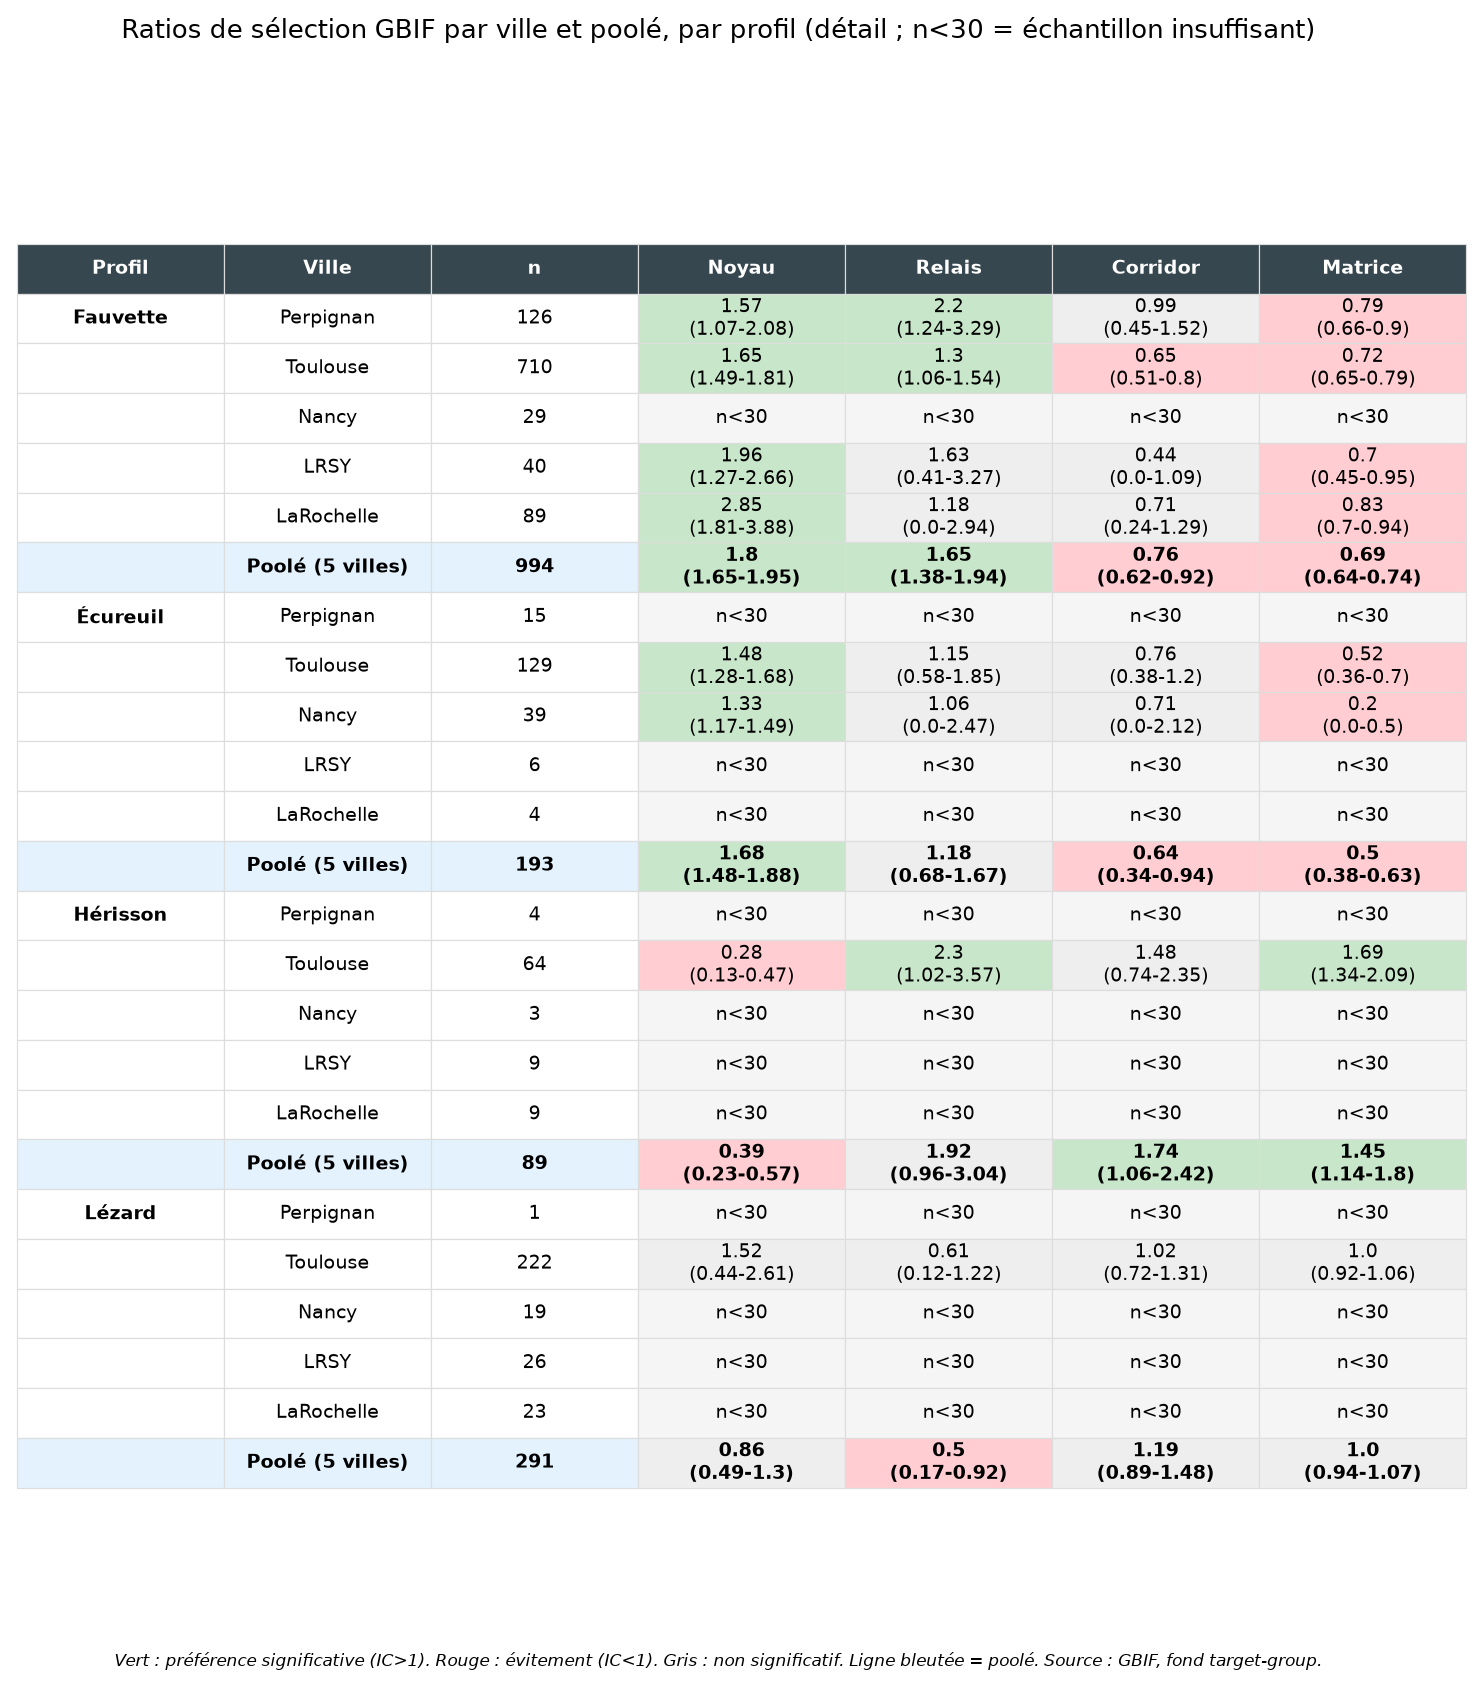
\includegraphics[width=0.98\textwidth]{figures/gbif_recap_par_ville.png}
\caption{Ratios de sélection GBIF par territoire et agrégés, par profil et par classe, avec intervalle de confiance à 95 \%. (d'après les données GBIF, 2026)}
\label{fig:21}
\end{figure}

Au-delà des ratios par classe, un test global du khi-deux à trois degrés de liberté vérifie, pour chaque profil, si les occurrences se répartissent entre les quatre classes différemment du fond d'observation. Le test compare, classe par classe, les effectifs observés de l'espèce focale à ceux qui seraient attendus si elle suivait exactement la répartition du fond d'observation (soit une absence de sélection) ; un écart trop grand pour être dû au hasard signale une sélection. La table de contingence a deux lignes (les effectifs de l'espèce focale et ceux du fond d'observation) et quatre colonnes (noyau, relais, corridor, matrice). La sélection est hautement significative pour l'oiseau de lisière, le mammifère arboricole et le petit mammifère terrestre, et non significative pour le reptile, pour lequel aucune sélection n'est détectée. Ces valeurs restent optimistes, le sous-échantillonnage spatial ne supprimant pas toute dépendance entre occurrences voisines \hyperref[sec:bibliographie]{(Legendre, 1993)}.

\begin{table}[H]
\centering
\begin{tabularx}{\textwidth}{>{\raggedright\arraybackslash}X >{\raggedright\arraybackslash}X >{\raggedright\arraybackslash}X >{\raggedright\arraybackslash}X >{\raggedright\arraybackslash}X}
\toprule
\textbf{Profil} & \textbf{Occurrences} & \textbf{khi-deux (3 ddl)} & \textbf{p} & \textbf{Sélection} \\
\midrule
Fauvette à tête noire & 994 & 166,2 & inférieur à 0,001 & significative \\
Écureuil roux & 193 & 44,1 & inférieur à 0,001 & significative \\
Hérisson d'Europe & 89 & 29,5 & inférieur à 0,001 & significative \\
Lézard des murailles & 291 & 4,5 & 0,21 & non significative \\
\bottomrule
\end{tabularx}
\end{table}

\section{Annexe C. Occurrences GBIF superposées aux noyaux, espaces relais et tracés de moindre coût, par profil}\label{annexe:C}

\begin{figure}[H]
\centering
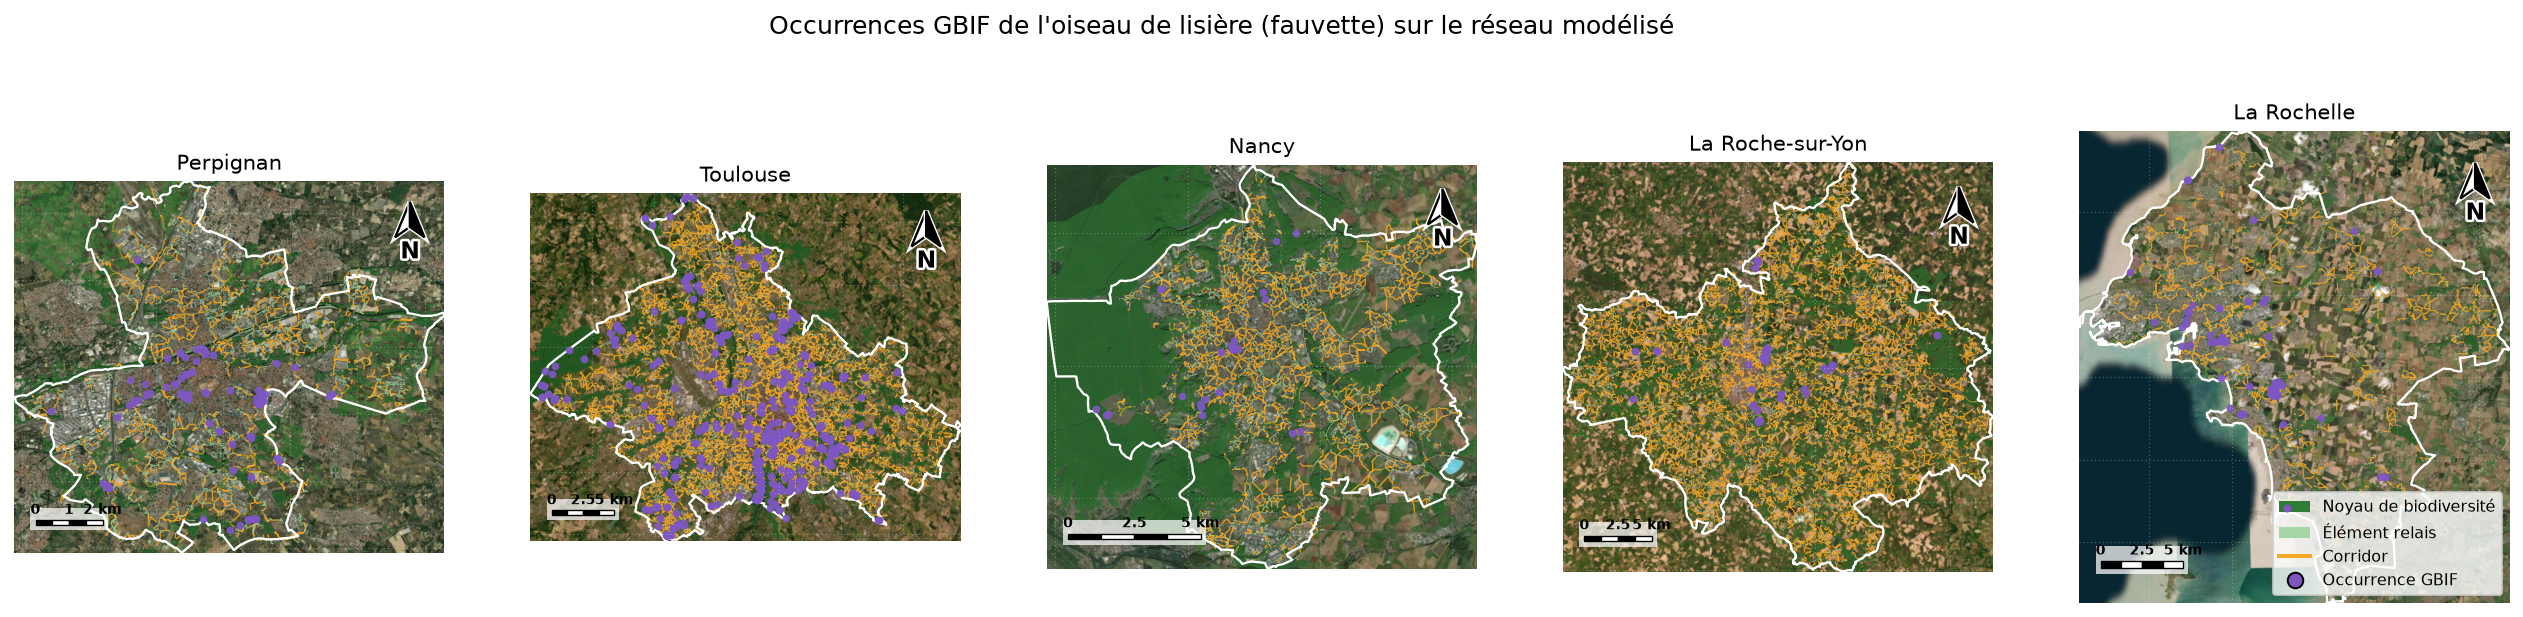
\includegraphics[width=0.98\textwidth]{figures/gbif_cartes_forest_edge_bird.png}
\caption{Cartes d'occurrences du profil des oiseaux de lisière (fauvette), un panneau par territoire. (d'après les données GBIF, 2026)}
\label{fig:22}
\end{figure}

\begin{figure}[H]
\centering
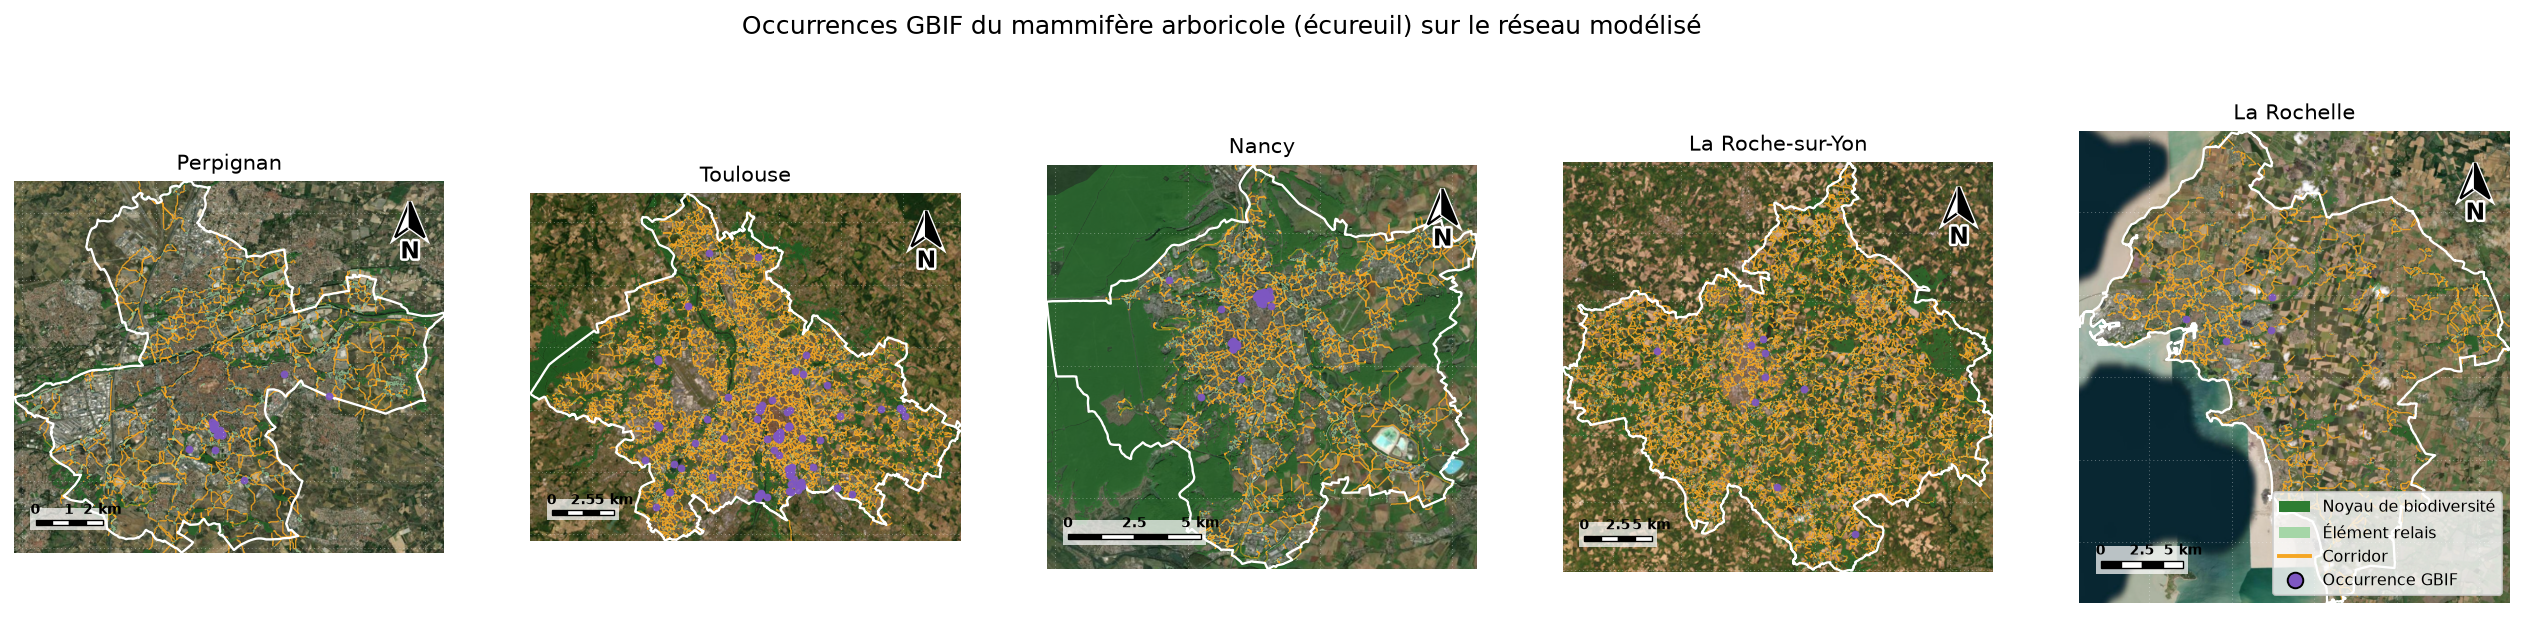
\includegraphics[width=0.98\textwidth]{figures/gbif_cartes_arboreal_mammal.png}
\caption{Cartes d'occurrences du profil des mammifères arboricoles (écureuil), un panneau par territoire. (d'après les données GBIF, 2026)}
\label{fig:23}
\end{figure}

\begin{figure}[H]
\centering
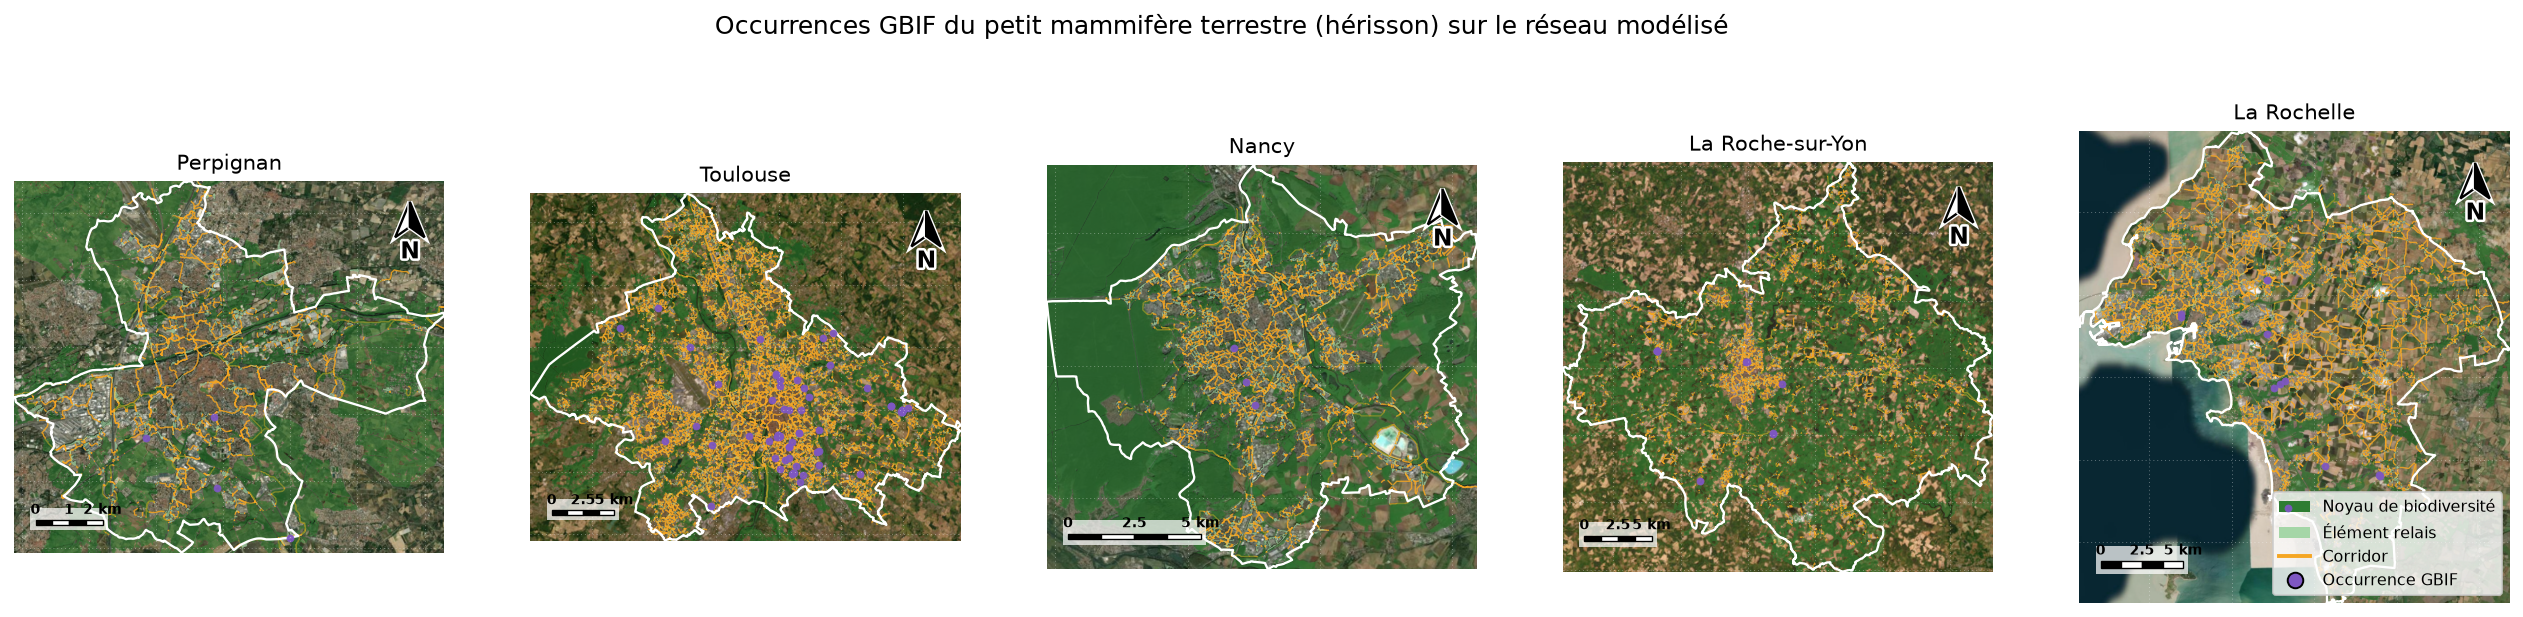
\includegraphics[width=0.98\textwidth]{figures/gbif_cartes_ground_mammal.png}
\caption{Cartes d'occurrences du profil des petits mammifères terrestres (hérisson), un panneau par territoire. (d'après les données GBIF, 2026)}
\label{fig:24}
\end{figure}

\begin{figure}[H]
\centering
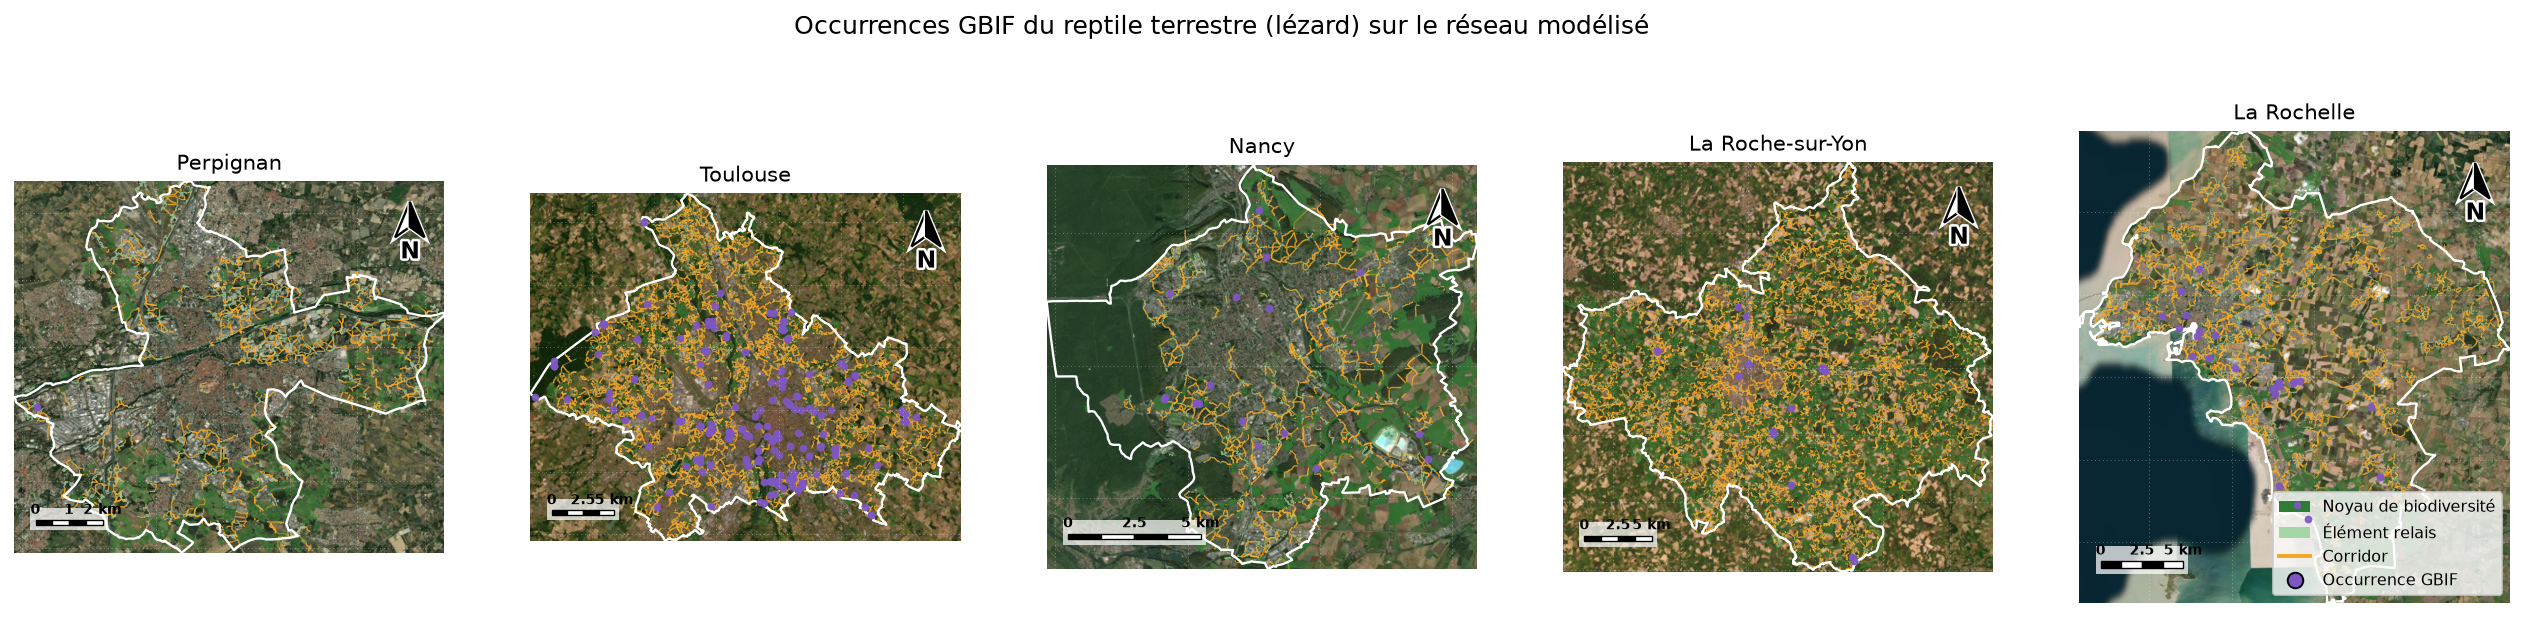
\includegraphics[width=0.98\textwidth]{figures/gbif_cartes_ground_reptile.png}
\caption{Cartes d'occurrences du profil des reptiles terrestres (lézard), un panneau par territoire. (d'après les données GBIF, 2026)}
\label{fig:25}
\end{figure}

\section{Annexe D. Indicateurs de connectivité par territoire et par profil écologique}\label{annexe:D}

La couverture d'habitat de la zone d'étude (proxy de végétalisation du territoire) est de 50 \% à La Roche-sur-Yon, 49 \% à Nancy, 39 \% à Perpignan, 53 \% à Kourou, 32 \% à Toulouse et 20 \% à La Rochelle. « Habitat connecté » = part d'habitat fonctionnellement connecté ; « sous-réseaux » = nombre de composantes connexes du réseau réel dans la zone d'étude ; « EC » = surface connectée équivalente.

\begin{table}[H]
\centering
\begin{tabularx}{\textwidth}{>{\raggedright\arraybackslash}X >{\raggedright\arraybackslash}X >{\raggedright\arraybackslash}X >{\raggedright\arraybackslash}X >{\raggedright\arraybackslash}X}
\toprule
\textbf{Territoire} & \textbf{Profil écologique} & \textbf{Habitat connecté} & \textbf{Sous-réseaux} & \textbf{EC (ha)} \\
\midrule
La Roche-sur-Yon & Petit mammifère terrestre & 83 \% & 1 & 20 864 \\
 & Mammifère arboricole & 28 \% & 1 & 2 747 \\
 & Oiseau de lisière & 19 \% & 1 & 1 932 \\
 & Reptile terrestre & 16 \% & 3 & 2 321 \\
Nancy & Petit mammifère terrestre & 71 \% & 1 & 4 916 \\
 & Mammifère arboricole & 56 \% & 1 & 2 676 \\
 & Oiseau de lisière & 52 \% & 1 & 2 468 \\
 & Reptile terrestre & 23 \% & 7 & 479 \\
Perpignan & Petit mammifère terrestre & 64 \% & 1 & 1 707 \\
 & Mammifère arboricole & 28 \% & 3 & 209 \\
 & Oiseau de lisière & 27 \% & 5 & 389 \\
 & Reptile terrestre & 23 \% & 14 & 270 \\
Kourou & Petit mammifère terrestre & 70 \% & 2 & 4 516 \\
 & Mammifère arboricole & 82 \% & 1 & 3 733 \\
 & Oiseau de lisière & 69 \% & 1 & 3 134 \\
 & Reptile terrestre & 45 \% & 4 & 852 \\
Toulouse & Petit mammifère terrestre & 52 \% & 1 & 7 674 \\
 & Mammifère arboricole & 27 \% & 1 & 2 445 \\
 & Oiseau de lisière & 21 \% & 3 & 1 965 \\
 & Reptile terrestre & 9 \% & 8 & 442 \\
La Rochelle & Petit mammifère terrestre & 40 \% & 1 & 2 632 \\
 & Mammifère arboricole & 17 \% & 11 & 253 \\
 & Oiseau de lisière & 15 \% & 28 & 223 \\
 & Reptile terrestre & 34 \% & 14 & 1 627 \\
\bottomrule
\end{tabularx}
\end{table}

\section{Annexe E. Analyse de sensibilité : synthèse par territoire et par profil écologique}\label{annexe:E}

\begin{quote}
Couverture : vingt-quatre couples, soit les six territoires par les quatre profils écologiques.
\end{quote}

\begin{landscape}
\begin{table}[H]
\centering
\footnotesize
\caption{Synthèse de sensibilité par territoire et par profil écologique : valeur de référence, plage sur le balayage de d$_{0}$ (50 à 120 \% de la référence) et plage sur le balayage du contraste de friction (0 à 200 \%).}
\begin{tabular}{llcccccc}
\toprule
\textbf{Territoire} & \textbf{Profil écologique} & \textbf{Connecté réf.} & \textbf{Connecté (d$_{0}$)} & \textbf{Connecté (contraste)} & \textbf{Sous-rés. réf.} & \textbf{Sous-rés. (d$_{0}$)} & \textbf{Sous-rés. (contraste)} \\
\midrule
Kourou & Petit mammifère terrestre & 70 \% & 69--70 \% & 70--97 \% & 2 & 2--3 & 1--2 \\
Kourou & Mammifère arboricole & 82 \% & 60--84 \% & 73--98 \% & 1 & 1 & 1 \\
Kourou & Oiseau de lisière & 69 \% & 51--75 \% & 57--96 \% & 1 & 1--2 & 1 \\
Kourou & Reptile terrestre & 45 \% & 42--47 \% & 43--61 \% & 4 & 3--8 & 1--7 \\
Perpignan & Petit mammifère terrestre & 64 \% & 52--68 \% & 54--96 \% & 1 & 1--3 & 1--2 \\
Perpignan & Mammifère arboricole & 28 \% & 20--30 \% & 21--74 \% & 3 & 1--12 & 1--10 \\
Perpignan & Oiseau de lisière & 27 \% & 21--30 \% & 21--77 \% & 5 & 3--22 & 1--18 \\
Perpignan & Reptile terrestre & 23 \% & 18--26 \% & 19--50 \% & 14 & 14--25 & 1--22 \\
Nancy & Petit mammifère terrestre & 71 \% & 55--74 \% & 60--96 \% & 1 & 1 & 1 \\
Nancy & Mammifère arboricole & 56 \% & 50--59 \% & 51--90 \% & 1 & 1--3 & 1 \\
Nancy & Oiseau de lisière & 52 \% & 46--54 \% & 47--88 \% & 1 & 1--5 & 1--4 \\
Nancy & Reptile terrestre & 23 \% & 19--25 \% & 20--51 \% & 7 & 2--26 & 1--22 \\
La Rochelle & Petit mammifère terrestre & 40 \% & 34--42 \% & 35--81 \% & 1 & 1--3 & 1--2 \\
La Rochelle & Mammifère arboricole & 17 \% & 15--18 \% & 15--38 \% & 11 & 7--47 & 1--42 \\
La Rochelle & Oiseau de lisière & 15 \% & 13--16 \% & 14--32 \% & 28 & 19--74 & 1--72 \\
La Rochelle & Reptile terrestre & 34 \% & 29--35 \% & 30--53 \% & 14 & 7--96 & 1--80 \\
La Roche-sur-Yon & Petit mammifère terrestre & 83 \% & 72--85 \% & 75--98 \% & 1 & 1 & 1 \\
La Roche-sur-Yon & Mammifère arboricole & 28 \% & 18--31 \% & 20--74 \% & 1 & 1--3 & 1--2 \\
La Roche-sur-Yon & Oiseau de lisière & 19 \% & 14--22 \% & 14--68 \% & 1 & 1--14 & 1--10 \\
La Roche-sur-Yon & Reptile terrestre & 16 \% & 11--18 \% & 12--51 \% & 3 & 3--13 & 1--11 \\
Toulouse & Petit mammifère terrestre & 52 \% & 38--55 \% & 41--91 \% & 1 & 1 & 1 \\
Toulouse & Mammifère arboricole & 27 \% & 20--28 \% & 21--72 \% & 1 & 1--5 & 1--4 \\
Toulouse & Oiseau de lisière & 21 \% & 17--23 \% & 17--66 \% & 3 & 2--23 & 1--19 \\
Toulouse & Reptile terrestre & 9 \% & 7--9 \% & 7--22 \% & 8 & 5--122 & 1--84 \\
\bottomrule
\end{tabular}
\end{table}
\end{landscape}

\end{document}
